% ---------------------------------------------------------------------
% --- Arquivo principal e os demais serao os dos capitulos.
% --- EXPRESSÔES ENTRE <> DEVERÂO SER COMPLETADAS COM A INFORMAÇÂO ESPECÌFICA DO TRABALHO 
% ---------------------------------------------------------------------

% Atualizado para atender as normas ABNT por Mônica da Silva (04/11/2021)

%configuração da entrada 
    % 12pt, 	% tamanho da fonte
    %openright, % capítulos começam em pág ímpar (insere página vazia caso preciso)
    % oneside, %% IMPRESSÃO dos elementos textuais e pós-textuais: oneside (apenas no anverso) ou twoside (anverso e verso, se mais de 100 p.) (insere páginas em branco).
    % a4paper, % tamanho do papel. 
    % english, % idioma adicional para hifenização
   	%english,			% idioma adicional para hifenização
	%french,				% idioma adicional para hifenização
	%spanish,			% idioma adicional para hifenização
	%brazil,				% o último idioma é o principal do documento

\documentclass[ruledheader, 12pt, openright, a4paper, oneside, english, brazil]{PPGC_UFF}



%---pacotes para hiphenizacao e acentuacao em portugues
\usepackage[brazil]{babel}
\usepackage[T1]{fontenc}
\usepackage[utf8]{inputenc}	
%\usepackage[latin1]{inputenc}
\usepackage{csquotes} % necessario para usar babel



%--- pacote para figuras
\usepackage{epsf, subfigure}
\usepackage[dvips]{epsfig,graphicx}
\usepackage{chngcntr} %configuração dos padrões numéricos das Figuras e Tabelas
\counterwithout{figure}{chapter} %formata figura para padrão: Figura 1.
\counterwithout{table}{chapter} %formata tabela para padrão: Tabela 1.


%--- pacote de simbolos
\usepackage{pifont,textcomp,latexsym}

%--- simbolos matematicos
\usepackage{amssymb,amstext,amsthm,icomma,amsmath}

%--- pacote para gerar pseudo-codigo
\usepackage{algorithm}
\usepackage{algorithmic}
\floatname{algorithm}{Algoritmo}

%--- outros pacotes
\usepackage{url}
\usepackage{longtable}
\usepackage{lscape}
\usepackage{quoting}

%Tabela Colorida
\usepackage{bigdelim,booktabs, colortbl, longtable, multirow, multicol,rotating }

%--- listagem de código
\usepackage{listings}
%\lstdefinestyle{sharpc}{language=[Sharp]C, frame=lr, rulecolor=\color{blue!80!black}}
%\lstset{style=sharpc}

\usepackage{comment}
%\begin{comment}
\definecolor{MyLightGray}{RGB}{200, 200,200}

\lstdefinelanguage{sharpc}
{
    columns=fullflexible,
    keywordstyle=\color{red},
    morekeywords={@prefix,@base,@forSome,@forAll,@keywords},
    morecomment=[l]{\#},
    tabsize=4, 
    alsoletter={-?}, % allowed in names
    morecomment=[s][\color{blue}]{<}{>},
    basicstyle=\ttfamily\color{black}, 
    %numberstyle=\color{black},
    morestring=[b][\color{black}]\",    
    backgroundcolor=\color{MyLightGray},
}
%\end{comment}

%--- pacote para incluir pdfs
\usepackage[final]{pdfpages}

%%===============================================================================
%% INICIO do Pacotes - Lista de abreviaturas, siglas e acrônimos
%%===============================================================================
		
% Modo "file": utiliza os termos definidos no arquivo acronimos.tex
%  1) Inserção tabular da listas
%  2) Controle da ordem de apresentação das listas
%  3) Não é preciso referenciar no texto
% nonumberlist, %do not show page numbers
% acronym,      %generate acronym listing   -> Not used in this example (see line with)
% toc,          % Inclui a abreviatura no sumário e conta pagina
% section]      %use section level for toc entries
\usepackage[acronym,nopostdot,shortcuts, nonumberlist]{glossaries}


\makeglossaries
\newacronym{DEE}{DEE}{Distância da pele até o espaço epidural}
\newacronym{IMC}{IMC}{Índice de Massa Corporal}
\newacronym{RU}{RU}{Reino Unido}
\newacronym{RV}{RV}{Realidade Virtual}
\newacronym{DoF}{DoF}{degrees of freedom}
\newacronym{ACR}{ACR}{Acronimos}

%%===============================================================================
%% FIM do Pacotes Lista de abreviaturas, siglas e acrônimos
%%===============================================================================

%%===============================================================================
%% Configuração das citações e personalização 
%%===============================================================================

% Os pacotes abaixo só podem ser usados juntamente com o pacote ABNT abaixo e na ordem atual. 
% Esse conjunto de pacotes permite que as citações fiquem na cor azul e sejam usadas como link para as referencias. 
\usepackage[bookmarksopen=true,
            linktoc=page, 
            colorlinks=true,  %ativa a cor do link na referencia
            linkcolor=blue, %muda a cor do link na referencia \ref{} números de tabelas, figuras, seções, sumário etc. 
            citecolor=blue, % muda a cor das citações \cite \textcite
            filecolor=magenta, 
            urlcolor=blue, %muda a cor da url \url no texto e ref. bibliográfica
            ]{hyperref}


\usepackage[ %mais informações de personalização das referencias olhar nos arquivos PDF na pasta MANUAIS OU https://www.overleaf.com/learn/latex/Biblatex_bibliography_styles
    %style = abnt, % Sistema alfabético
    style = abnt-numeric, % Sistema numérico
    %style = abnt-ibid, % Notas de referência
    language=brazil,
    backend=biber,
    maxnames=10, 
    %minnames=1, 
    %nohashothers=false,
]{biblatex}

\addbibresource{bibliografia.bib} % A biblioteca para ser utilizada na dissertação/tese.

%%===============================================================================
%% FIM da configuração das citações e personalização 
%%===============================================================================

\hyphenation{
a-de-qua-da-men-te 
di-men-sio-na-men-to 
}

%---------usando tipo de fonte padrão  
% mathptmx (títulos sem negrito) ou ptm (títulos negrito)  - Times - Padrão 
% ugq (títulos negrito) - Arial 
%% --  Padrão do template é: ptm  -- %%
\renewcommand{\ABNTchapterfont}{\bfseries\fontfamily{ptm}\fontseries{b}\selectfont} 
\renewcommand{\ABNTsectionfont}{\bfseries\fontfamily{ptm}}


% --- -----------------------------------------------------------------
% --- Documento Principal.
% --- -----------------------------------------------------------------

\begin{document}


% --- -----------------------------------------------------------------
% --- Titulo, abstract, dedicatórias e agradecimentos.
% --- Índice geral, lista de figuras e tabelas.
% --- -----------------------------------------------------------------
% Atualizado para atender as normas ABNT por Mônica da Silva (04/11/2021)

% --- -----------------------------------------------------------------
% --- Elementos usados na Capa e na Folha de Rosto.
% --- EXPRESSÔES ENTRE <> DEVERÂO SER COMPLETADAS COM A INFORMAÇÂO ESPECÍFICA DO TRABALHO
% --- E OS SÌMBOLOS <> DEVEM SER RETIRADOS 
% --- -----------------------------------------------------------------
\autor{RAFAEL HEITOR CORREIA DE MELO} % deve ser escrito em maiúsculo

\titulo{Uma Proposta de Uso de Dispositivo Háptico
para Treinamento de Anestesia Raquidiana}

\instituicao{UNIVERSIDADE FEDERAL FLUMINENSE}

\orientador{Aura Conci, D.Sc.}

%\coorientador{<NOME DO COORIENTADOR>} % se nao existir co-orientador apague essa linha

\local{NITER\'{O}I}

\data{2022} % ano da defesa

\comentario{Tese de Doutorado apresentada ao Programa de P\'{o}s-Gradua\c{c}\~{a}o em Computa\c{c}\~{a}o da \mbox{Universidade} Federal Fluminense como requisito parcial para a obten\c{c}\~{a}o do Grau de \mbox{Doutor em Computa\c{c}\~{a}o}. \'{A}rea de concentra\c{c}\~{a}o: \mbox{Computação Visual.}} %preencha com a sua área de concentração


% --- -----------------------------------------------------------------
% --- Capa. (Capa externa, aquela com as letrinhas douradas)(Obrigatório)
% --- ----------------------------------------------------------------
\capa

% --- -----------------------------------------------------------------
% --- Folha de rosto. (Obrigatório)
% --- ----------------------------------------------------------------
\folhaderosto

% --- -----------------------------------------------------------------
% --- Ficha catalográfica obrigatória na versão final. (Obrigatório)
% --- ----------------------------------------------------------------

\begin{figure}[!ht]
   \centering
   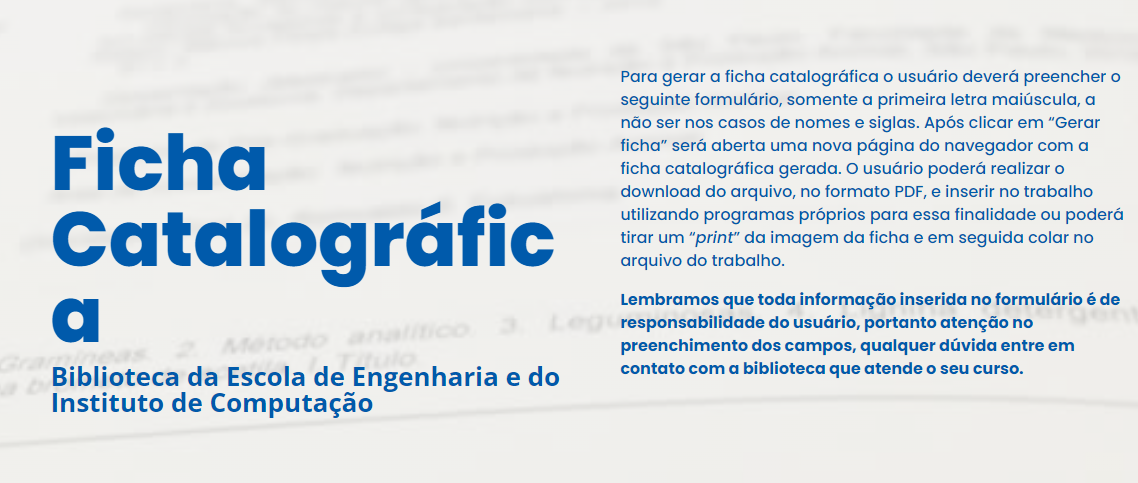
\includegraphics[width=1\linewidth]{capitulos/figuras/ficha_catalografica.png}
   \caption{Local da ficha catalográfica}
\end{figure}

\cleardoublepage


\pagestyle{ruledheader}
\setcounter{page}{1}
\pagenumbering{roman}

% --- -----------------------------------------------------------------
% --- Termo de aprovação. (Obrigatório)
% --- ----------------------------------------------------------------
\cleardoublepage
\thispagestyle{empty}

\vspace{-60mm}

\begin{center}
   {\large RAFAEL HEITOR CORREIA DE MELO}\\
   \vspace{7mm}

   Uma Proposta de Uso de Dispositivo Háptico
para Treinamento de Anestesia Raquidiana\\
  \vspace{10mm}
\end{center}

\noindent
\begin{flushright}
\begin{minipage}[t]{8cm}

Tese de Doutorado apresentada ao Programa de P\'{o}s-Gradua\c{c}\~{a}o em Computa\c{c}\~{a}o da Universidade Federal Fluminense como requisito parcial para a obten\c{c}\~{a}o do \mbox{Grau} de Doutor em Computa\c{c}\~{a}o. \'{A}rea de concentra\c{c}\~{a}o: \mbox{Ciência da Computação.} %preencha com a sua área de concentração

\end{minipage}
\end{flushright}
\vspace{1.0 cm}
\noindent
Aprovada em outubro de 2022. \\
\begin{flushright}
 % \parbox{11cm}
  {
  \begin{center}
  BANCA EXAMINADORA \\
  \vspace{6mm}
  \rule{11cm}{.1mm} \\
    Profa. D.Sc. Aura Conci - Orientadora, UFF \\
    \vspace{6mm}
  \rule{11cm}{.1mm} \\
    Prof. D.Sc. Anselmo Cardoso de Paiva, UFMA\\
    \vspace{6mm}
  \rule{11cm}{.1mm} \\
    Prof. D.Sc. Débora Christina Muchaluat Saade, UFF\\
  \vspace{4mm}
  \rule{11cm}{.1mm} \\
    Prof. D.Sc. Fátima de Lourdes dos Santos Nunes Marques, USP\\
    \vspace{6mm}
  \rule{11cm}{.1mm} \\
    Prof. D.Sc. José Viterbo Filho, UFF\\
  \vspace{6mm}
  \end{center}
  }
\end{flushright}
\begin{center}
  \vspace{4mm}
  Niter\'{o}i \\
  %\vspace{6mm}
  2022

\end{center}

% --- -----------------------------------------------------------------
% --- Dedicatoria.(Opcional)
% --- -----------------------------------------------------------------
\cleardoublepage
\thispagestyle{empty}
\vspace*{200mm}

\begin{flushright}
{\em 
    %Dedicatória(s): Elemento opcional onde o autor presta homenagem ou dedica seu trabalho (ABNT, 2005).
    
    Dedico este trabalho a minha esposa, Evelyn, que sempre me apoiou na direção das minhas conquistas e ao meu filho, Rafael, que, ao chegar me apresentou uma nova forma de amar.
}
\end{flushright}
\newpage


% --- -----------------------------------------------------------------
% --- Agradecimentos.(Opcional)
% --- -----------------------------------------------------------------
\pretextualchapter{Agradecimentos}
\hspace{5mm}
%<Elemento opcional, colocado após a dedicatória (ABNT, 2005). >
Agradeço a Deus por me mostrar sempre os caminhos, mesmo nos momentos em que parece que isso não vai acontecer. 

Aos meus pais Julio e Dayse pela preocupação e apoio. Aos meus irmãos Leonardo e Julia pela amizade e companheirismo essenciais nos momentos difíceis.

Agradeço muito a minha orientadora Aura, que mesmo nos momentos de desânimo conseguiu me trazer, em palavras, motivação para seguir em frente.

Ao amigo André que foi essencial em parte dessa caminhada.

À minha família, agradeço a compreensão pelas minhas ausências e minhas desculpas nos momentos de desânimo.



% --- -----------------------------------------------------------------
% --- Resumo em português.(Obrigatório)
% --- -----------------------------------------------------------------
\begin{resumo}

%Elemento obrigatório, constituído de uma sequência de frases concisas e objetivas e não de uma simples enumeração de tópicos, não ultrapassando 500 palavras ABNT NBR 6028:2003.

As anestesias raquidianas são procedimentos cegos que dependem do sentimento do médico no decorrer da inserção da agulha para correta identificação do local de aplicação do líquido anestésico. Em grande parte dos centros de treinamento a primeira experiência tátil do médico em treino tende a ser praticada em pacientes reais. Esta prática, apesar de ser efetuada sob supervisão direta, traz riscos para estes pacientes e inseguranças aos aprendizes. Técnicas alternativas de uso de \textit{phantoms} e cadáveres no treinamento oferecem uma pequena representatividade em relação às variações de pacientes reais. 
Nesta tese desenvolvemos um ambiente virtual para simulação do procedimento que envolve anestesias raquidianas. Considera-se o procedimento de punção com \textit{feedback} tátil e visual usando técnicas de autotreinamento. As sensações táteis do médico em treinamento são simuladas no protótipo através da integração com dispositivo háptico. A geração e visualização dinâmica de modelos de corpos de pacientes baseados em altura e peso foi desenvolvida a partir de uma criteriosa revisão bibliográfica de trabalhos anteriores sendo uma parte muito importante deste trabalho. Alunos de computação validaram a parte do protótipo que envolve a detecção de diferentes sensações de perfuração de tecidos por meio de experimentos propostos. Ainda foi criado e usado aqui um modelo adaptável de um corpo de gestante que possui modelagem de todas as camadas desde a pele das costas até os ossos da coluna vertebral. Modelamos de forma dinâmica as camadas de tecido mais variáveis para permitir uma maior variabilidade de cenários de treinamento. Finalmente, incluímos também uma variação das etapas de treinamento de acordo com a detecção automática do nível de habilidade da pessoa na execução de cada procedimento. Pessoas com execução insatisfatória terão que executar mais procedimentos durante o seu treinamento. Os erros são reportados durante cada procedimento para possibilitar a evolução na prática do aprendiz.

{\hspace{-8mm} \bf{Palavras-chave}}: Dispositivo háptico, Treinamento médico, Anestesia raquidiana, Realidade virtual, Ambiente virtual, Paciente virtual Simulação, Retorno tátil.

\end{resumo}

% --- -----------------------------------------------------------------
% --- Resumo em língua estrangeira.(Obrigatório)
% --- -----------------------------------------------------------------
\begin{abstract}

%Elemento obrigatório, em língua estrangeira, com as mesmas características do resumo em língua vernácula (ABNT, 2005).

Spinal anesthesia is a blind procedure where physicians rely on manual feedback to guide their movements through needle insertion. The aim is to identify drug administration locations correctly. For many training centers, the first tactile experience of anesthetists in training occurs in an actual patient under direct supervision. Besides this supervision, there are risks associated with this approach for patients and apprentices. Using phantoms and dead bodies for training offers a low range of scenarios. In this thesis, we developed a virtual environment for simulating the procedure that involves spinal anesthesia. The puncture procedure is considered with tactile and visual feedback using self-training techniques. The tactile sensations of the physician in training are simulated in the prototype through integration with a haptic device. The dynamic generation and visualization of models of patients' bodies based on height and weight was developed from a careful bibliographic review and is a significant part of this work. Computer science students validated the detection of different sensations of tissue perforation related to the procedure through experiments. An adaptable model of a pregnant woman's body was created and used here. We include in the model all layers from the skin of the back to the spine's bones. To allow more significant variability of training scenarios, we included the dynamic possibility of growth to most variable tissue layers. Finally, we also included a variation of the training steps according to the automatic detection of the person's skill level in performing each procedure. People with poor execution will have to perform more procedures during their training. Errors are reported during each procedure to allow progress in the learner's practice. 



% O resumo deve ser redigido na terceira pessoa do singular, com verbo na voz ativa, não ultrapassando uma página ou 500 palavras, segundo a ABNT NBR 6028). Evitando-se ouso de parágrafos no meio do resumo, assim como fórmulas, equações e símbolos. Iniciar o resumo situando o trabalho no contexto geral, apresentar os objetivos, descrever a metodologia utilizada, relatar a contribuição própria, comentar os resultados obtidos e finalmente apresentaras conclusões mais importantes do trabalho. 



{\hspace{-8mm} \bf{Keywords}}: Haptics, Medical training, Spinal anesthesia, Virtual reality, Virtual environment, Virtual patient, Simulation, tactile feedback.

\end{abstract}

% --- -----------------------------------------------------------------
% --- Lista de figuras.(Opcional)
% --- -----------------------------------------------------------------
%\cleardoublepage
\listoffigures



% --- -----------------------------------------------------------------
% --- Lista de tabelas.(Opcional)
% --- -----------------------------------------------------------------
\cleardoublepage
%\label{pag:last_page_introduction}
\listoftables
\cleardoublepage

% --- -----------------------------------------------------------------
% --- Lista de abreviatura.(Opcional)
%Elemento opcional, que consiste na relação alfabética das abreviaturas e siglas utilizadas no texto, seguidas das %palavras ou expressões correspondentes grafadas por extenso. Recomenda-se a elaboração de lista própria para cada %tipo (ABNT, 2005).
% --- ----------------------------------------------------------------

\cleardoublepage
\printglossary[type=\acronymtype,title={Lista de Abreviaturas e Siglas}]
\cleardoublepage


% --- -----------------------------------------------------------------
% --- Sumario.(Obrigatório)
% --- -----------------------------------------------------------------

\pagestyle{ruledheader}
\tableofcontents
\pagebreak %na pasta capítulos

% --- -----------------------------------------------------------------
% --- Inserção dos capítulos.
% --- todos os arquivos estão na pasta capítulos
% --- -----------------------------------------------------------------

\setcounter{page}{1} %parâmetros da contagem de paginas.
\pagenumbering{arabic} %padrão de números de paginas em arábico (1,2,3) 
\setcounter{page}{12} %inicia a contagem das paginas 12 - folha de rosto e considera a pagina da 

\pagestyle{ruledheader}

%%%% CAPÍTULO 1 - INTRODUÇÃO
%%
%% Deve apresentar uma visão global da pesquisa, 
%% incluindo: breve histórico, importância e
%% justificativa da escolha do tema, delimitações
%% do assunto, formulação de hipóteses e objetivos
%% da pesquisa e estrutura do trabalho.

% Perguntas que podem guiar a introdução - não necessariamente irá ter a resposta para tudo, isso depende da área.
% 1 - Qual é o contexto em que seu trabalho está inserido?
% 2 - Qual é o problema que motiva a existência deste trabalho?
% 3 - Qual é a visão geral da literatura sobre o problema e como é tratado
% 4 - Por que a solução na literatura não é o suficiente para ?
% 5 - Como seu trabalho trata o problema ?
% 6 - como seu trabalho foi avaliado para comprovar que tratou adequadamente o problema?
% 7 - De forma geral quais foram os resultados ?
% 8 - Quais foram as contribuições do seu trabalho?
% 9 -  Como o restante da Dissertação ou Tese está organizada ?


\chapter{Introdução}
\label{cap:introducao}

Nas anestesias raquidianas os anestesistas dependem da sua sensação tátil durante a inserção da agulha no paciente para a correta identificação do local de aplicação do líquido anestésico. O local de aplicação da raquidiana é conhecido como espaço subaracnóideo \cite{Miller2009}). Para que o anestesista reconheça a chegada da agulha neste local ele precisa reconhecer os tecidos perfurados no caminho dela. As anestesias possuem técnicas específicas para identificação dos seus espaços de aplicação. Para que os médicos dominem a técnica da anestesia raquidiana é estimado que são necessários 44 ± 6 repetições de execução deste tipo de procedimento \cite{Kopacz1996}. A confirmação de que o local adequado foi atingido na anestesia raquidiana é feita através da observação do vazamento, por meio da agulha de punção, do liquido cérebro espinhal ou cefalorraquidiano (\textit{líquor}). As Figuras~\ref{fig:puncaoLombar} e~\ref{fig:gotejamentoLiquor} ilustram dois momentos importantes da anestesia raquidiana retirados do vídeo de \textcite{Londero2018} disponível no link\footnote{\url{https://www.youtube.com/watch?v=Dl8ijvHVTuY&ab_channel=CLAUDINEILONDERO}}. Na Figura~\ref{fig:puncaoLombar} é mostrado o momento de inserção da agulha para punção lombar e na Figura~\ref{fig:gotejamentoLiquor} é mostrado o vazamento, através da agulha de punção, do \textit{líquor}, o que acontece alguns segundos após a agulha estar corretamente posicionada no espaço subaracnóideo. Neste tipo de anestesia é usada uma agulha de menor diâmetro do que a agulha utilizada na anestesia epidural \cite{Miller2009}. O ultrassom é uma ferramenta eficiente para auxílio na determinação do espaço onde a agulha precisa ser inserida \cite{Helayel2010, Soni2019} bem como na definição da espessura das diversas camadas de tecido \cite{Klingensmith2022}. Existem inclusive soluções desenvolvidas para interpretação de imagens de ultrassom que vem sendo estudadas para substituir a apalpação do anestesista na determinação do ponto de inserção da agulha \cite{Ni2021}. Porém, o uso de equipamentos de ultrassom para este fim não é uma realidade em muitos centros no Brasil \cite{Hamaji2016}. O uso deste equipamento ou qualquer outra técnica \cite{Berde2022}, portanto não faz parte do treinamento de muitas faculdades de medicina para anestesias raquidianas. A determinação do ponto de inserção da agulha no treinamento, assim como no procedimento real em pacientes, é comumente feita fazendo uso de referências anatômicas através da apalpação da crista ilíaca do paciente. A crista ilíaca pode ser observada nas imagens da Figura~\ref{fig:cristaIliaca} \cite{Moura2019}. 

\begin{figure}[!ht]
   \centering
   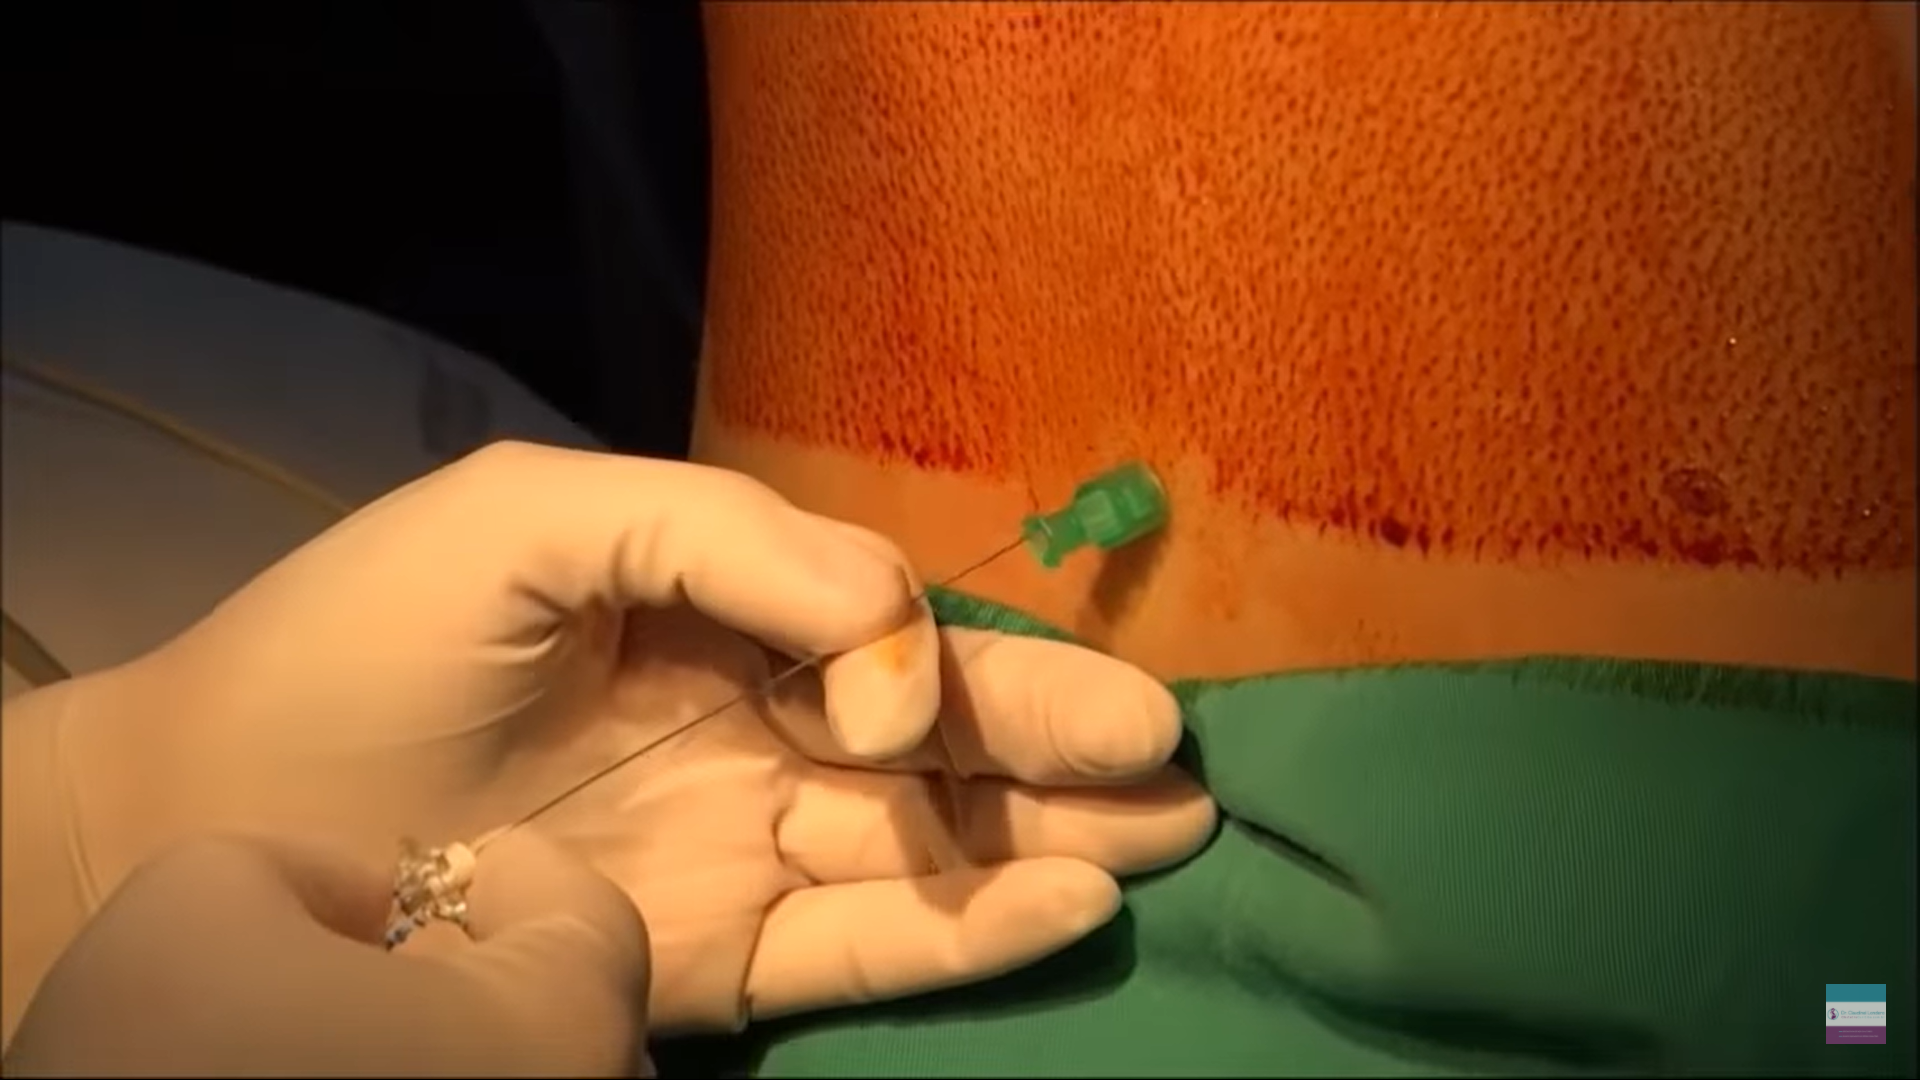
\includegraphics[width=0.6\linewidth]{capitulos/figuras/2.PuncaoLombar.png}
   \caption{Punção lombar com agulha de raquianestesia  \cite{Londero2018}.}
   \label{fig:puncaoLombar}
\end{figure}

\begin{figure}[!ht]
   \centering
   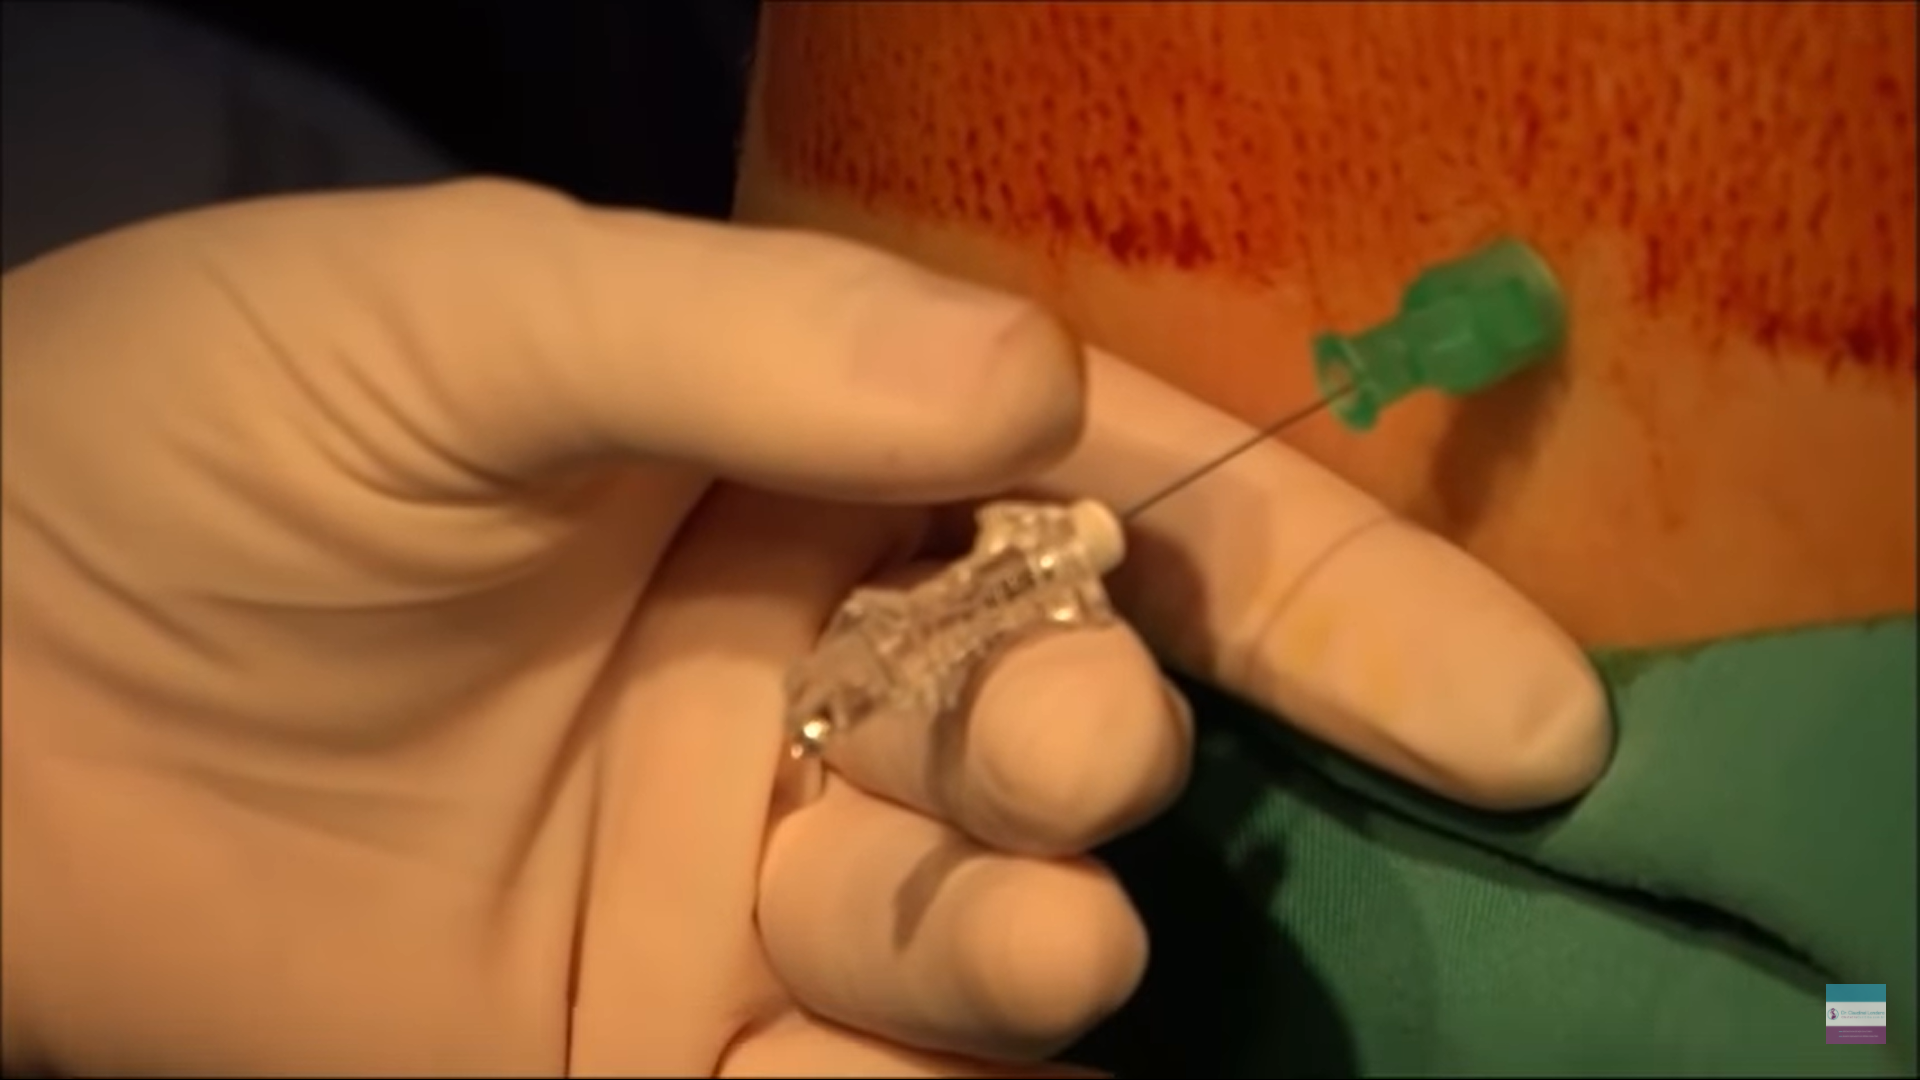
\includegraphics[width=0.6\linewidth]{capitulos/figuras/3.GotejamentoLiquor.png}
   \caption{Gotejamento do \textit{líquor}, indicação do local correto para a raquianestesia \cite{Londero2018}.}
   \label{fig:gotejamentoLiquor}
\end{figure}

\begin{figure}[ht!]
    \centering
        \begin{tabular}{cc}
        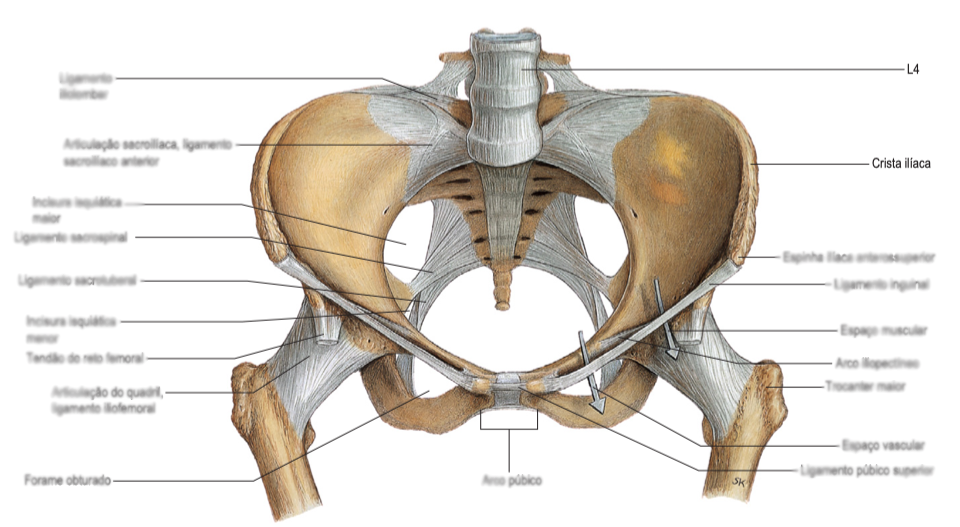
\includegraphics[width=0.55\linewidth]{capitulos/figuras/crista-iliaca-pelve-ossos-ligamentos.png} & 
        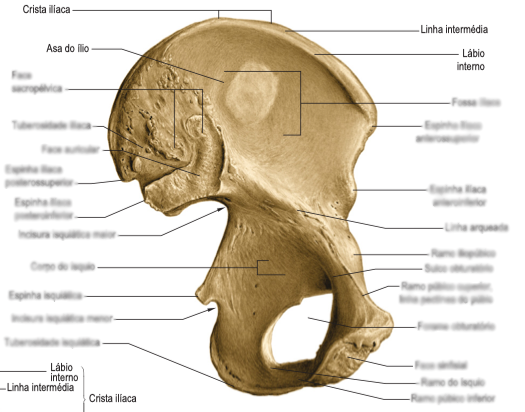
\includegraphics[width=0.35\linewidth]{capitulos/figuras/crista-iliaca-ossos-quadril.png} 
        \\
        (a) & (b)
        \end{tabular}
    \caption{Ilustração da crista ilíaca através de duas imagens dos ossos da pelve \cite{Moura2019}. Nas imagens a indicação de elementos que não estão diretamente relacionados à crista ilíaca foram embaçados de forma a simplificar a visualização desta: (a) Vista frontal (b) Vista lateral.}
    \label{fig:cristaIliaca}
\end{figure}

A principal abordagem de treinamento para técnicas de anestesia envolve a observação da aplicação das técnicas por anestesistas experientes \cite{Vrillon2022}. Estes orientam verbalmente os aprendizes conforme cada um dos passos é executado. Adicionalmente a isto são usados: desenhos 2D, cadáveres para demonstração do procedimento, apresentação de vídeos das técnicas sendo executadas em pacientes, visualização 3D \cite{Vrillon2022} e técnicas de simulação. No que diz respeito ao treinamento das sensações táteis além do uso de cadáveres alguns simuladores fazem uso de bonecos com tecidos artificiais, denominados \textit{phantoms}, que simulam pacientes \cite{Dreifaldt2006, KyotoKagaku2015, Mashari2018}. Um ponto negativo importante no uso de \textit{phantoms} e de cadáveres, talvez o principal, é a baixa representatividade no que diz respeito a reprodução da situação real, pois estes oferecem uma baixa variabilidade de cenários (variações possíveis dos corpos dos pacientes) para treinamento. Esta fato fica notório na análise destes tipos de simuladores feita na Seção \ref{sec:SimuladoresPhantoms}. A maior quantidade de tipos de corpos representado pelos \textit{phantoms} nos simuladores estudados foi de 4 enquanto é sabido que a variabilidade das estruturas corporais mesmo em uma população pequena é muito maior do que isso. Outro aspecto relevante no uso de \textit{phantoms} é a necessidade de reposição de peças que se desgastam com o uso e podem ter custos altos. Estes são alguns dos motivos para que em diversos hospitais a primeira experiência do anestesista em treinamento seja efetuada diretamente em um paciente \cite{Aggarwal2009, Grantcharov2008, Smith2005, Watterson2007}. Esta prática, apesar de ser efetuada sob supervisão direta de médicos experientes, pode trazer riscos para as pessoas que são anestesiadas (pacientes) e uma maior propensão a inseguranças por parte dos aprendizes \cite{Elmofty2017}. 

O uso de simuladores para adquirir certo grau de habilidade antes de iniciar o procedimento em pacientes minimiza os riscos tanto para o aprendiz quanto para o paciente não só na anestesia \cite{Escobar-Castillejos2016, Yunoki2018} como em diversas outras áreas da medicina \cite{Akhtar2014, Alvarez-Lopez2020, Hamm2022}. A existência de diversos cenários em simuladores como os que usam \acrfull{RV} auxilia e motiva o ensino e possibilita ao aprendiz ter experiência com situações mais variadas assim como aumenta a segurança dos alunos. Essa técnica tem também a vantagem de possibilitar que a avaliação do desempenho destes seja feita de forma automatizada e padronizada \cite{Willis2014}. 

Estes simuladores com frequência usam diferentes níveis variando as dificuldades \cite{Ullrich2012}. Possibilitam a redução ou eliminação de custos de manutenção de equipamentos e laboratórios físicos bem como evitam a necessidade de estruturação de laboratórios \cite{Silva2018}. 
Esta variabilidade de cenários dificilmente aconteceria na vida real em centros onde o ensino é feito diretamente em pacientes \cite{Udani2015}. No cenário de treinamento diretamente em pacientes a experiência inicial de cada anestesista pode ser muito distinta uma vez que estas dependem da estrutura corporal do paciente atendida por cada residente. Esta não é uma abordagem ideal para treinamentos uma vez que cria uma dependência no que diz respeito à experiência tátil dos anestesistas novatos em uma variável que não está sob o controle do profissional responsável pelo treinamento. Cada aluno pode vir a ter uma gama diferente de experiências a depender das características físicas dos pacientes que este teve suas primeiras experiências. Isto impacta o nivelamento do ensino.

Diversos simuladores utilizam dispositivos de força háptica (\textit{force feedback}) para auxiliar o aprendiz a experimentar fisicamente as sensações de resistência modeladas para os tecidos ao praticar procedimentos médicos. Este tipo de abordagem é usada em procedimentos médicos de um modo geral \cite{Escobar-Castillejos2016, Patel2021} assim como no caso mais específico dos procedimentos de anestesia \cite{Vaughan2013, Collaco2021}. Existem muitas outras formas de como o uso de ferramentas computacionais pode auxiliar no campo da anestesia. Um exemplo é no controle automatizado de quanto anestésico aplicar a partir de respostas de medições dos níveis de consciência do paciente \cite{Mendez2009}. Outro exemplo é uso da imersão \acrshort{RV} durante a cirurgia em conjunto com a anestesia como forma de reduzir a dor e estimular o relaxamento diminuindo a ansiedade e possivelmente a quantidade de anestésico necessário \cite{Eijlers2019}.

\textcite{Correa2019}, na sua análise do estado da arte, relataram que as avaliações da percepção humana são pouco exploradas no campo da interação háptica para treinamento de inserção de agulhas. Eles também citam a predominância de testes subjetivos para validação das soluções propostas por parte dos usuários. Alguns trabalhos fazem uso de análises subjetivas usando gráfico de profundidade da agulha versus tempo como em \textcite{Magill2010}. 

O trabalho desta tese foi iniciado com a apresentação do simulador de \textcite{Brazil2017thesis} para um anestesista com o intuito de agregar a este simulador outro tipo de anestesia, no caso a anestesia raquidiana. A proposta inicial desta tese propunha a utilização destes simuladores para a avaliação de ganho de conhecimento no treinamento de novos anestesistas com o uso do simuladores em comparação com a ausência do seu uso. A opinião do especialista foi a de que este tipo de avaliação seria mensurável de forma mais concreta para o simulador de raquianestesia. A partir de estudos do estado da arte foi observado que os simuladores que possibilitam a anestesia raquidiana não contemplam algumas das principais características desejáveis para a correta representação do procedimento como por exemplo a apalpação da coluna para determinação do ponto de inserção da agulha. Com isto um simulador de anestesia raquidiana foi construído visando atender as principais demandas do treinamento das sensações envolvidas neste procedimento. Na literatura estudada foram adotadas diversas formas de abordar o problema do treinamento de anestesias regionais. Simuladores deste tipo possuem muitas características relevantes o que faz com que o foco no atendimento em algumas geralmente venha a comprometer outras. Grande parte dos simuladores computacionais de anestesia estudados apresenta como opção para o usuário somente a simulação de anestesias epidurais e não de raquianestesias que é o foco desta tese.

A apresentação de cenários de treinamento virtuais que simulam a possibilidade de visualização e sentimentos táteis que são vivenciados no procedimento real visa aproximar a prática de treino virtual da posterior prática em pacientes reais. Desta forma, possibilita um maior sentimento de segurança por parte dos anestesistas aprendizes. A aplicação de transparência em camadas foi uma das técnicas que foi incluída no ambiente virtual de treinamento criado nesta tese. Esta funcionalidade permite a visão do interior do corpo o que facilita o entendimento do aprendiz no que diz respeito à teoria do procedimento. Esta conexão da teoria com a prática é um grande trunfo no uso da \acrfull{RV} em simuladores para treinamento. Neste caso, o realismo na apresentação dos elementos envolvidos no treinamento tem um papel importante. Seja a representação 3D da agulha, do corpo ou das camadas internas que possam ser visualizadas. 

\section{Definição do problema}
\newtheorem{prob}{Problema}

Esta tese de doutorado define a seguinte questão de pesquisa a ser estudada e solucionada por este trabalho.

\begin{prob}
\label{prob:simuladorCasoReal}
    É possível criar uma ferramenta virtual para treinamento médico que auxilie no treinamento do procedimento de raquianestesia a partir do uso de realidade virtual e com dispositivo háptico de forma a simular este procedimento desde a palpação da coluna (para determinação do ponto de inserção da agulha)?
\end{prob}

Dentre os simuladores de raquianestesia computacionais atuais não existe um que contemple na simulação a palpação do corpo pelo médico anestesista para determinação do ponto de inserção da agulha. Esta opção existe para somente dois simuladores de anestesia epidurais estudados nesta tese sendo que somente em um deles este procedimento é feito de maneira 100\% virtual como propomos neste trabalho. O simulador epidural que possibilita simulação de apalpação não teve a sua solução avaliada por especialistas. 

\section{Objetivos}
\label{sec:objetivos}

Esta tese tem o seguinte objetivo geral:

Propor e desenvolver um ambiente de treinamento virtual no que se refere às técnicas de anestesia raquidiana em gestantes desde a apalpação para determinação do ponto de inserção da agulha até a administração do anestésico no local correto. A ideia é prover um aprendizado prático, didático e mais completo dos anestesistas sem incorrer em risco para os pacientes e estresse para os anestesistas em treinamento. Este treinamento será padronizado no sentido das técnicas que precisarão ser dominadas pelos usuários treinados. O sistema irá fazer com que os usuários que demonstrarem melhor desenvoltura nas etapas iniciais evoluam mais rapidamente pelas etapas de demonstração de habilidades já entendidas e aprendidas. 

Dentre os objetivos específicos pode-se destacar:
\begin{enumerate}
\item Possibilitar variações das situações possíveis de ocorrer em relação às características físicas das pacientes; 
\item Desenvolver modelagens que mapeiam as características físicas na visualização; 
\item Possibilitar visualização dos tecidos internos no momento da anestesia para auxílio no aprendizado inicial. 
\item Utilizar técnicas de realidade virtual na representação da paciente e dos equipamentos usados no procedimento em ambiente 3D interativo;
\item Empregar dispositivos hápticos como meio de interação para simular os sentimentos táteis do médico (de forma semelhante ao procedimento real em treinamento);
\item Dar retorno ao usuário em relação as ações feitas corretas e incorretas no que diz respeito ao procedimento visando auxiliar na evolução do seu desempenho.
\end{enumerate}

\section{Contribuições da Tese}
\label{sec:contribuicoes}

Uma das principais contribuições deste trabalho envolve a reprodução virtual das principais sensações hápticas necessárias para simular a anestesia raquidiana. Outra contribuição foi a construção de um modelo 3D real da parte lombar do corpo de uma gestante (tecidos entre a pele e a cauda equina) de forma facilmente modificável via programação. A variação dos tamanhos das principais camadas do modelo foi alimentada por um equação genérica criada e detalhada neste trabalho. Foi criado então um ambiente para treinamento de raquianestesia que apresenta \textit{feedbacks} durante e após cada
procedimento bem como uma proposta de avaliação de desempenho por meio de notas.

\section{Estrutura da Tese}
\label{sec:estrutura}

O restante do texto está estruturado da seguinte forma. O Capítulo~\ref{cap:cap2} comenta os principais conceitos e tecnologias envolvidas no desenvolvimento do ambiente de treinamento proposto.

O Capítulo~\ref{cap:cap3} contém os trabalhos relacionados a esta tese assim como o posicionamento deste trabalho frente aos demais.

No Capítulo~\ref{cap:cap4} é apresentada a especificação do ambiente de treinamento que foi desenvolvido durante esta tese. 

A implementação do ambiente de treinamento que foi desenvolvido durante esta tese está descrita no Capítulo~\ref{cap:cap5}. 

O Capítulo~\ref{cap:cap6} apresenta os experimentos que foram feitos e uma avaliação destes em relação aos seus resultados.

Por fim, o Capítulo~\ref{cap:cap7} conclui o trabalho, apresentando as conclusões, realçando as contribuições desta tese e apontando as limitações e os  trabalhos futuros.




\pagestyle{ruledheader}
\chapter{Fundamentação Teórica} \label{cap:cap2}

Este Capítulo relaciona os conceitos e as tecnologias envolvidas no desenvolvimento do ambiente de treinamento proposto. 

\section{Anestesias Regionais}

Anestesias são atualmente usadas em diversos procedimentos cirúrgicos na medicina tradicional com o intuito de bloquear temporariamente a capacidade do cérebro de reconhecer um estímulo doloroso. Esta prática visa permitir a execução de procedimentos invasivos por parte do médico enquanto mantém o conforto e a tranquilidade do paciente. A anestesia regional é um procedimento usado em cirurgias onde o paciente pode permanecer acordado. Este tipo de anestesia bloqueia a dor em apenas uma determinada região do corpo, como um braço, uma perna ou toda região inferior do corpo, abaixo do abdômen \cite{Pinheiro2018}.

Os dois tipos de anestesias regionais mais usados são: anestesia raquidiana (ou raquianestesia, raqui), e anestesia peridural ou epidural. Estes dois tipos de anestesias também são conhecidas como anestesias de neuroeixo ou ainda bloqueio de neuroeixo \cite{Pinheiro2018}. Ambas podem ser aplicadas com pacientes sentados e inclinados para frente ou deitados de lado \cite{Anesclin2019}. 

\begin{figure}[ht!]
    \centering
    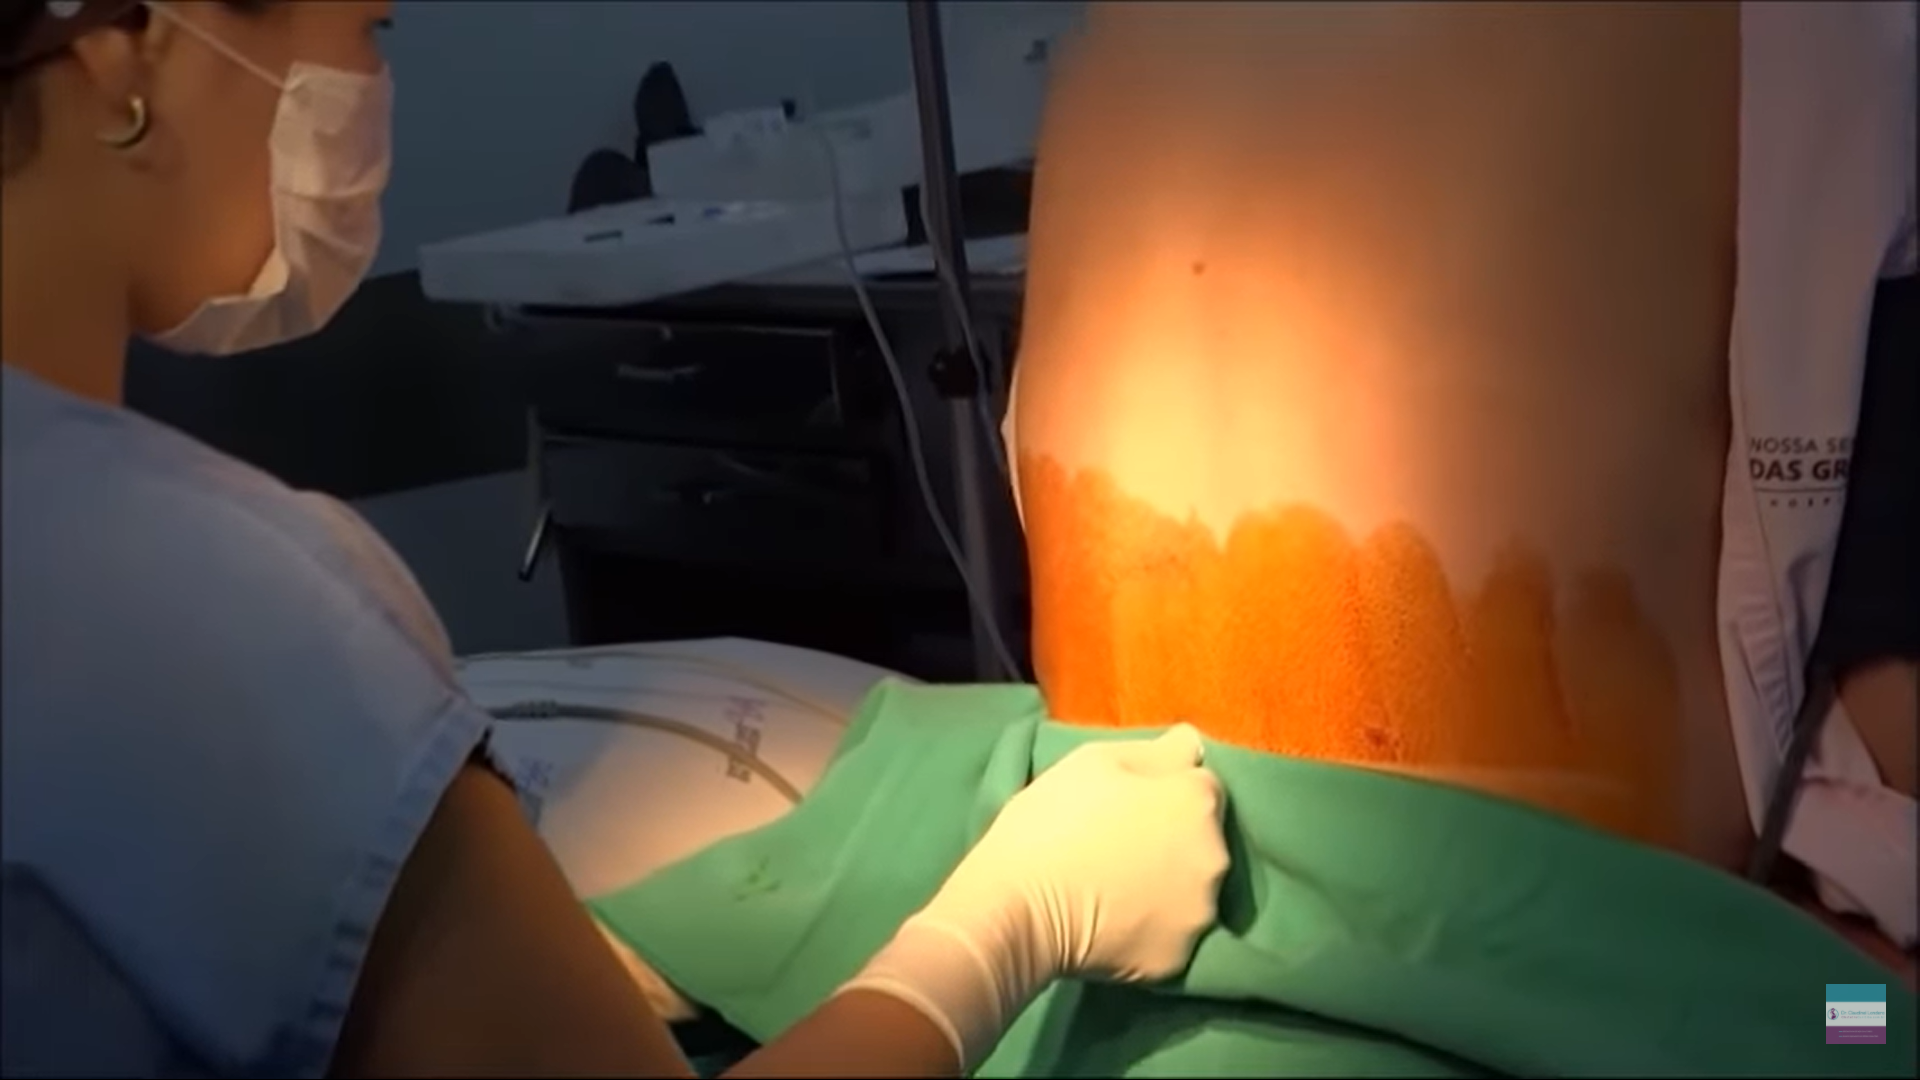
\includegraphics[width=0.6\linewidth]{capitulos/figuras/0.marcacaoPonto.png}
    \caption{Palpação para determinação do ponto de inserção da agulha \cite{Londero2018}.}
    \label{fig:marcacaoPonto}
\end{figure}

\begin{figure}[ht!]
    \centering
    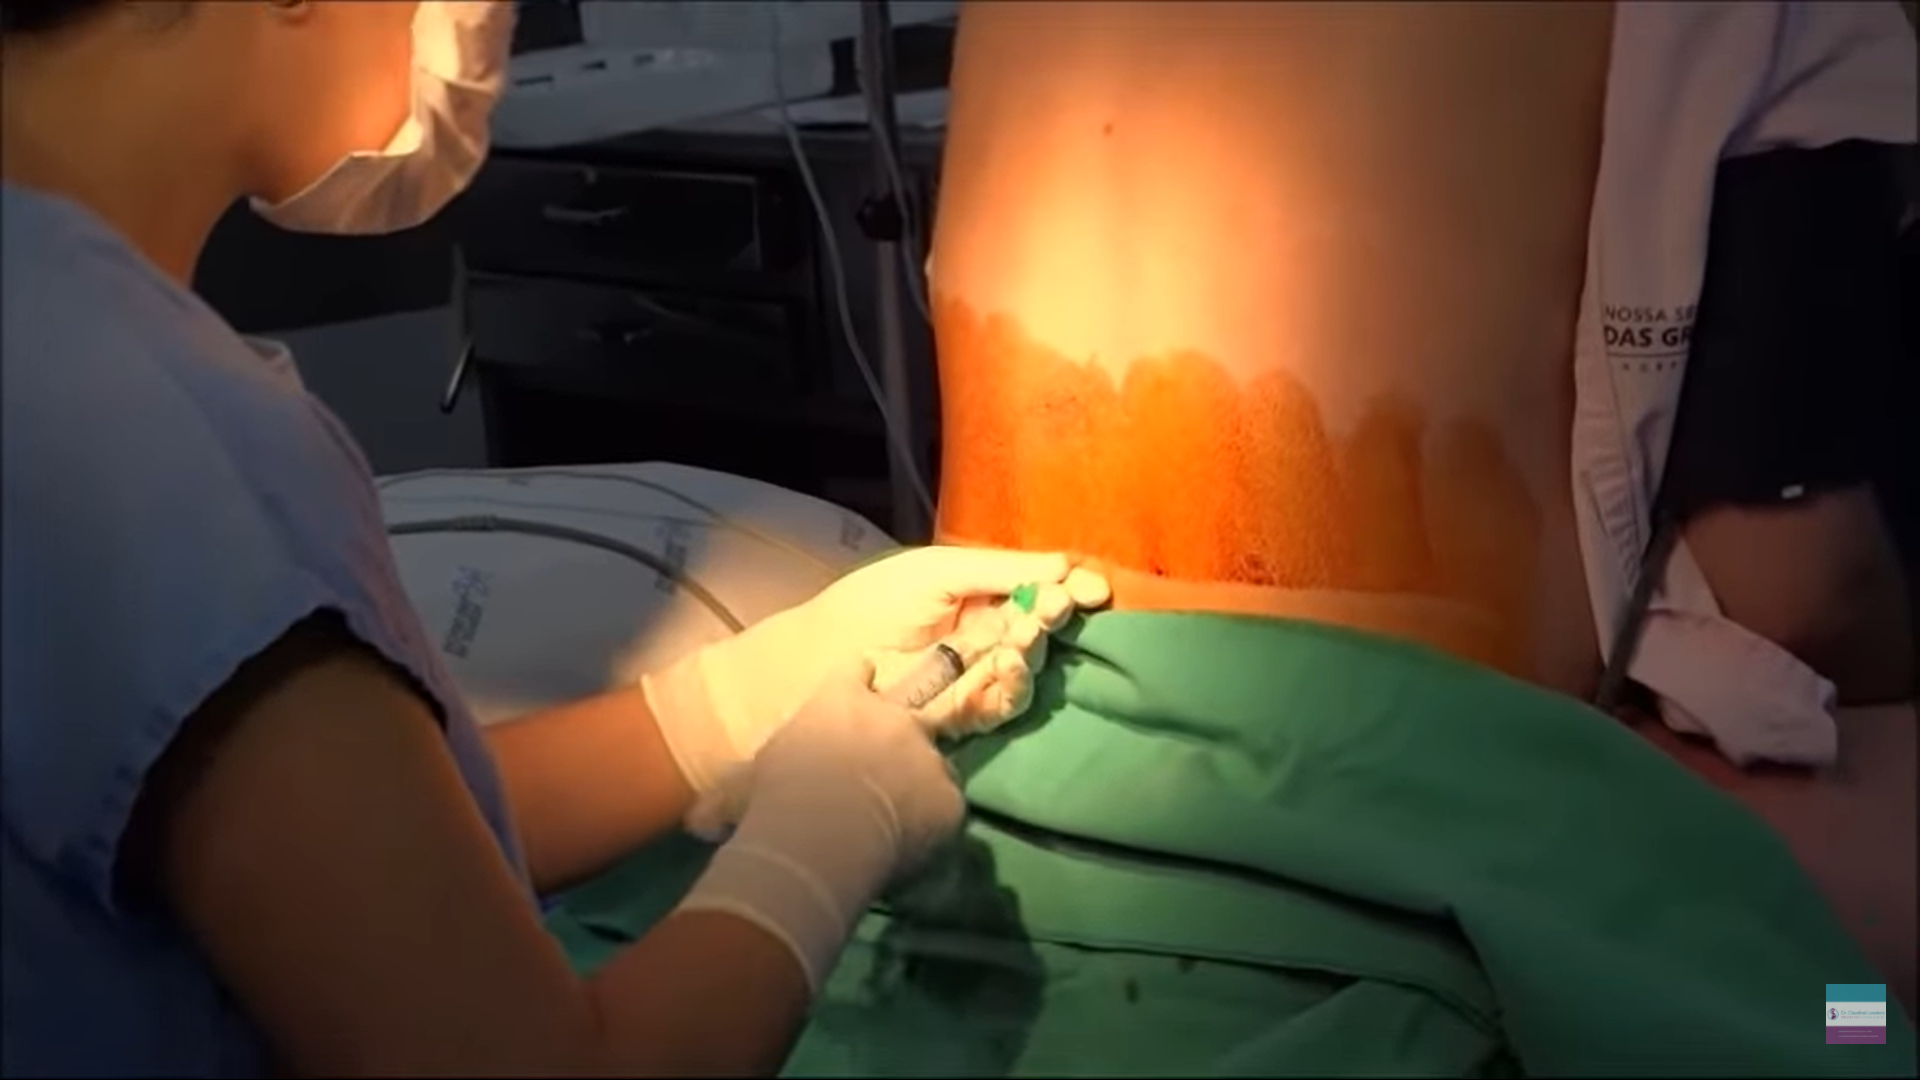
\includegraphics[width=0.6\linewidth]{capitulos/figuras/1.AnestesiaLocal.png}
    \caption{Aplicação da anestesia local \cite{Londero2018}.}
    \label{fig:anestesiaLocal}
\end{figure}

\begin{figure}[ht!]
    \centering
    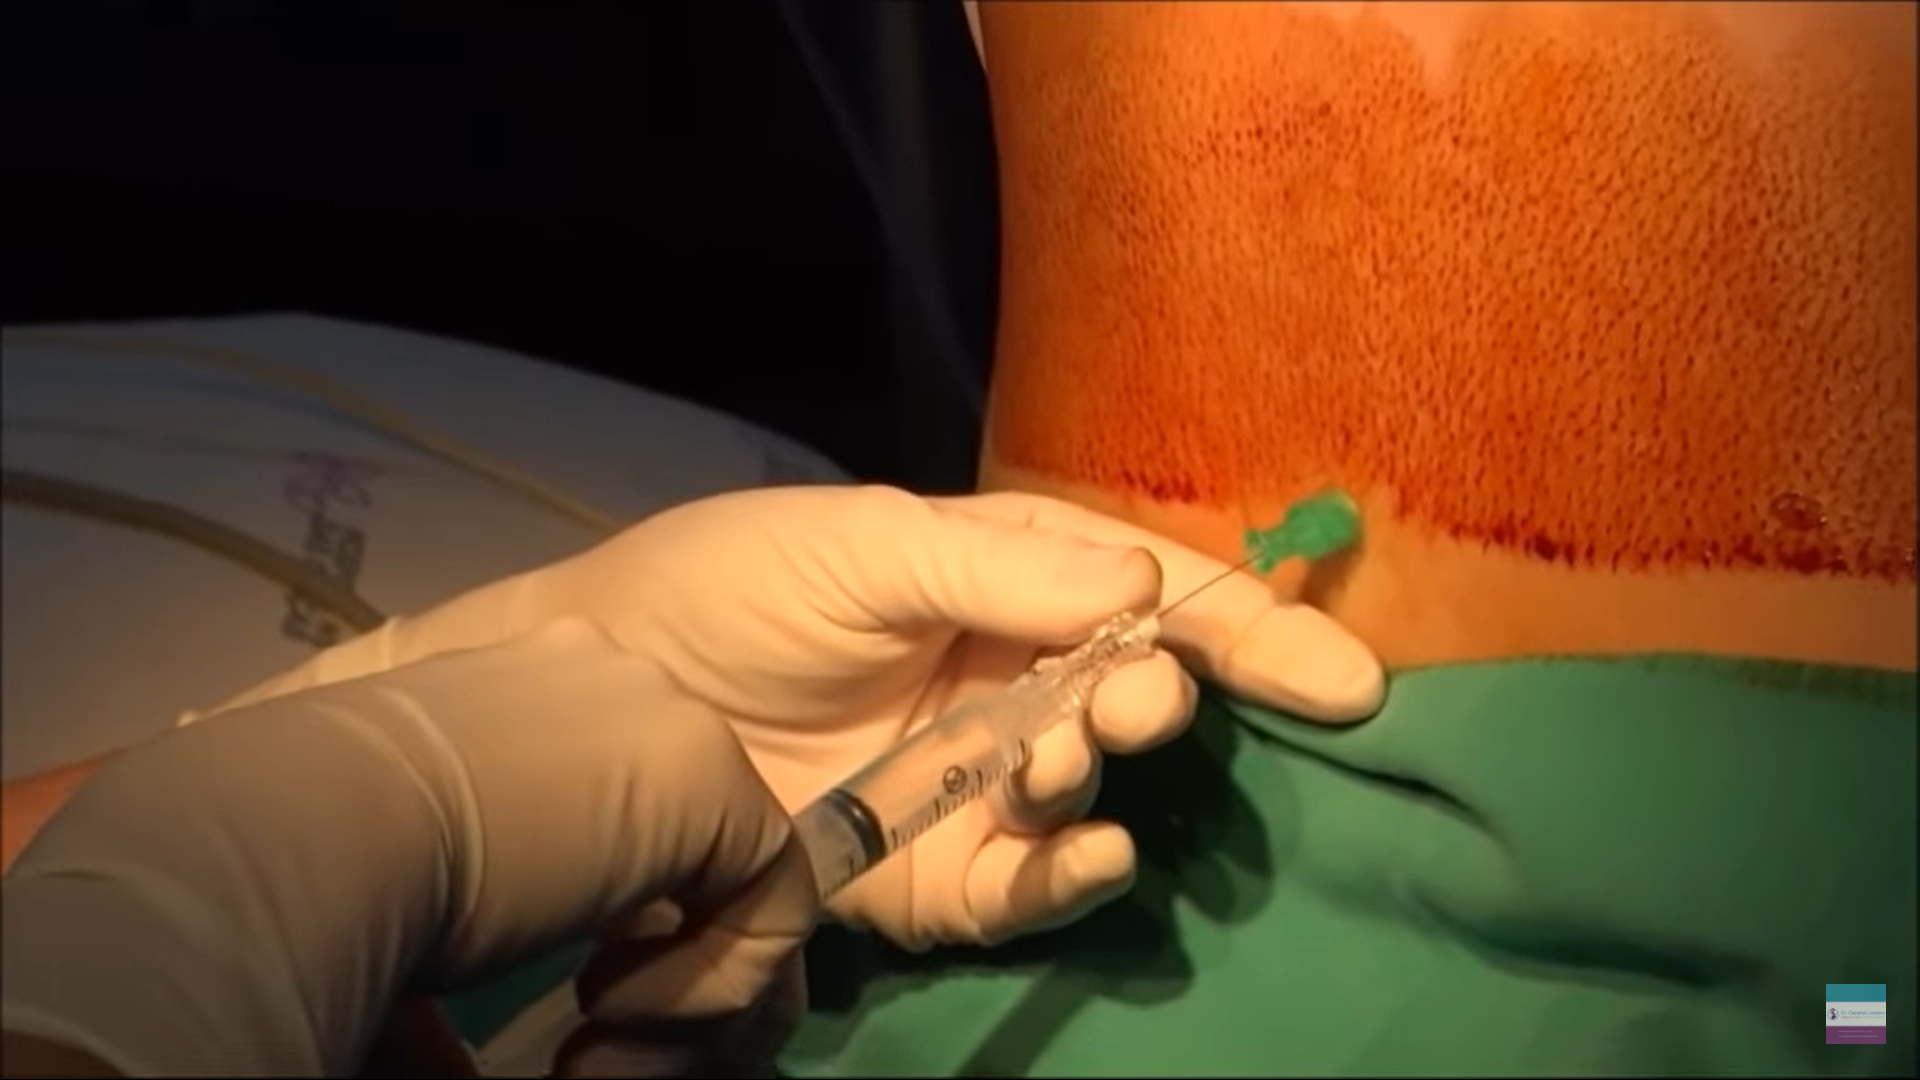
\includegraphics[width=0.6\linewidth]{capitulos/figuras/4.InjecaoAnestesico.png}
    \caption{Injeção do liquido anestésico no espaço subaracnóideo  \cite{Londero2018}.}
    \label{fig:injecaoAnestesico}
\end{figure}

Após a finalização dos procedimentos de preparação é escolhida a área onde será feita a punção através do toque da mão do médico (exemplo retirado de video na Figura~\ref{fig:marcacaoPonto}) na crista ilíaca do paciente \cite{Helayel2010,Isaacs2015}. Uma vez escolhido este ponto é feita a injeção de anestésico local (Figura~\ref{fig:anestesiaLocal}) para reduzir o desconforto na área próxima à punção \cite{Sedicias2018} Após a anestesia local é feita a inserção da agulha de punção tanto no caso da peridural como na raqui.

Existem duas principais abordagens de inserção da agulha para efetuação das anestesias regionais. Estão são denominadas mediana (do inglês \textit{midline}) e paramediana (do inglês \textit{paramedian}). A abordagem mediana é utilizada com mais frequência (96\%) \cite{Wantman2006}. Um dos motivos para o maior uso da abordagem mediana é a ausência de vasos sanguíneos no caminho da agulha nesta abordagem \cite{Bapat2015}. A abordagem paramediana é mais recomendada para pacientes idosos \cite{Ahsan-ul-Haq2005} por motivos de modificação degenerativa da coluna vertebral \cite{Boon2003} e calcificação dos ligamentos interespinhoso e supraespinhoso \cite{Wantman2006}. A abordagem paramediana também pode ser mais viável que a mediana em pacientes obesos pela dificuldade na identificação da crista ilíaca nestes pacientes. Isto por que a camada de gordura faz com que a linha média seja mais difícil de localizar através do toque do médico \cite{N.2013}. Na abordagem mediana a agulha é inserida na linha média da coluna vertebral. Na paramediana existe certa angulação entre a linha da coluna e a inserção da agulha. As duas abordagens podem ser observadas no corte transversal da coluna na Figura~\ref{fig:abordagensInsercaoAgulha}. 

\begin{figure}[ht!]
    \centering
    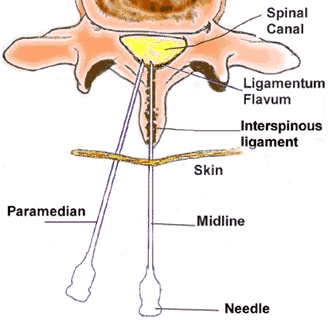
\includegraphics[width=0.6\linewidth]{capitulos/figuras/paramedian-midline-MedBroadcast-Tiff.png}
    \caption{Ilustração da abordagem mediana e paramediana para inserção de agulha \cite{MedBroadcast2018}.}
    \label{fig:abordagensInsercaoAgulha}
\end{figure}

\subsection{Anestesia Raquidiana}

Neste tipo de anestesia, uma agulha de pequeno calibre é inserida nas costas do paciente até atingir o espaço subaracnóideo (localizado após a dura-máter), dentro da coluna espinhal. Em seguida, um anestésico é injetado dentro do líquido cérebro espinhal (\textit{líquor}), produzindo dormência temporária e relaxamento muscular (Figura~\ref{fig:injecaoAnestesico}). Anestesias raquidianas são aplicadas de forma mais frequente em espaços intervertebrais abaixo da segunda vértebra lombar (L2), normalmente entre a L3 e L4 \cite{Wikipedia2019, Londero2018}. A Figura~\ref{fig:camadasPuncaoLombar} ilustra em um corte sagital da coluna as diferentes camadas que são cruzadas por uma agulha durante o procedimento de punção lombar até chegar ao espaço subaracnóideo. Considerando as duas abordagens de inserção da agulha (mediana e paramediana) as camadas onde a agulha pode passar desde a pele até o espaço subaracnóideo são: gordura subcutânea, músculo, ligamento supraespinhoso, ligamento interespinhoso, ligamento amarelo (\textit{flavum}), espaço epidural e dura-máter. O processo espinhoso que também aparece entre a pele e o espaço subaracnóideo na Figura~\ref{fig:camadasPuncaoLombar} não foi listado, pois, por ser uma camada de osso, ela não é perfurada pela agulha e sim uma camada intransponível em relação ao processo de punção.

\begin{figure}[ht!]
    \centering
    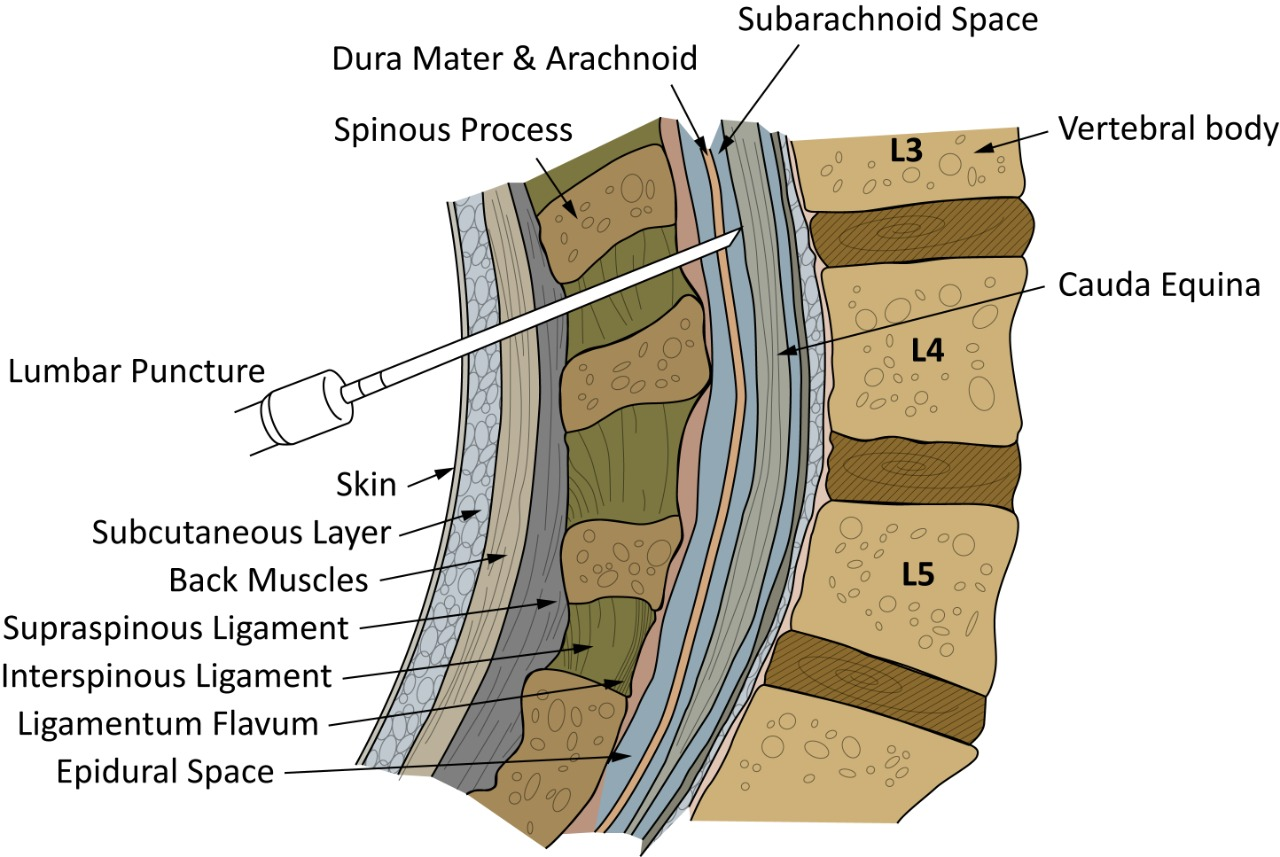
\includegraphics[width=0.6\linewidth]{capitulos/figuras/lumbar.puncture.tisssues.jpeg}
    \caption{Camadas cruzadas pela agulha numa punção lombar.}
    \label{fig:camadasPuncaoLombar}
\end{figure}

A ação do anestésico dentro da coluna espinhal é a de bloquear os nervos que passam pela coluna lombar, fazendo com que os estímulos dolorosos vindos de membros inferiores e do abdômen não cheguem ao cérebro. A raquianestesia é muito usada para procedimentos ortopédicos de membros inferiores assim como na região abdominal e cirurgias obstétricas de parto normal e cesarianas \cite{Pinheiro2018}.

A grande vantagem da anestesia raquidiana em relação a peridural é que nesta é necessário o uso de uma pequena quantidade de anestésico local. Esta característica reduz consideravelmente o risco de intoxicação por meio do elemento anestésico. Por outro lado a maior desvantagem no uso deste tipo de anestesia está na dor de cabeça que os pacientes sentem após a perfuração da dura-máter. Este sintoma é causado pela lesão na dura-máter que pode permanecer aberta por alguns dias após o procedimento, provocando perda do \textit{líquor} do espaço subaracnóideo. Com o uso de agulhas de menor diâmetro a incidência desta dor de cabeça foi consideravelmente reduzida \cite{INFOESCOLA2018}. 

\section{Realidade Virtual}

A \acrlong{RV} está presente quando se usa a tecnologia para criar a ilusão de que se está em um ambiente que não está lá ou não existe. Ela é uma aproximação da realidade experimentada por nós através dos nossos sentidos e sistemas de percepção. A nossa percepção da realidade vem através dos nossos sentidos. Portanto, uma vez apresentando aos sentidos às informações esperadas, sendo estas reais ou não, a nossa percepção da realidade irá se guiar por estes estímulos. Os sentidos mais comuns são visão, olfato, paladar, audição e tato. Porém também possuímos outros sentidos que afetam as nossas percepções do mundo, como por exemplo: o senso de equilíbrio, o sentimento de forças, pesos e deslocamentos sentidos por nossos membros \cite{VRS2018}.

Atualmente, a chamada \acrfull{RV} utiliza um computador para criar um ambiente virtual tridimensional. A intenção é a de simular uma realidade apresentando os elementos desejáveis para os sentidos do usuário, visando cumprir um objetivo através da interação de um ou mais usuários com este ambiente. Estes usuários se tornam parte deste ambiente virtual, total ou parcialmente, podendo manipular objetos ou executar um conjunto de ações \cite{VRS2018}.

A \acrshort{RV} possui uma série de usos sociais como, por exemplo, o tratamento de fobias. Há trabalhos para aracnofobia \cite{Carlin1997}, para aicmofobia ou medo de agulhas \cite{Galoustian2018}, para aerofobia ou medo de voar \cite{Rothbaum2006}, para acrofobia ou medo de altura \cite{Edwards2018} ou de forma mais geral para o medo e a ansiedade \cite{Goldman2017}. A Figura~\ref{fig:medoAltura} ilustra a aplicação para tratamento da acrofobia. Em primeiro plano a usuária com os óculos de realidade virtual e no segundo plano o ambiente virtual simulando ambientes de escadas e plataformas com fundo transparente.

\begin{figure}[ht!]
    \centering
    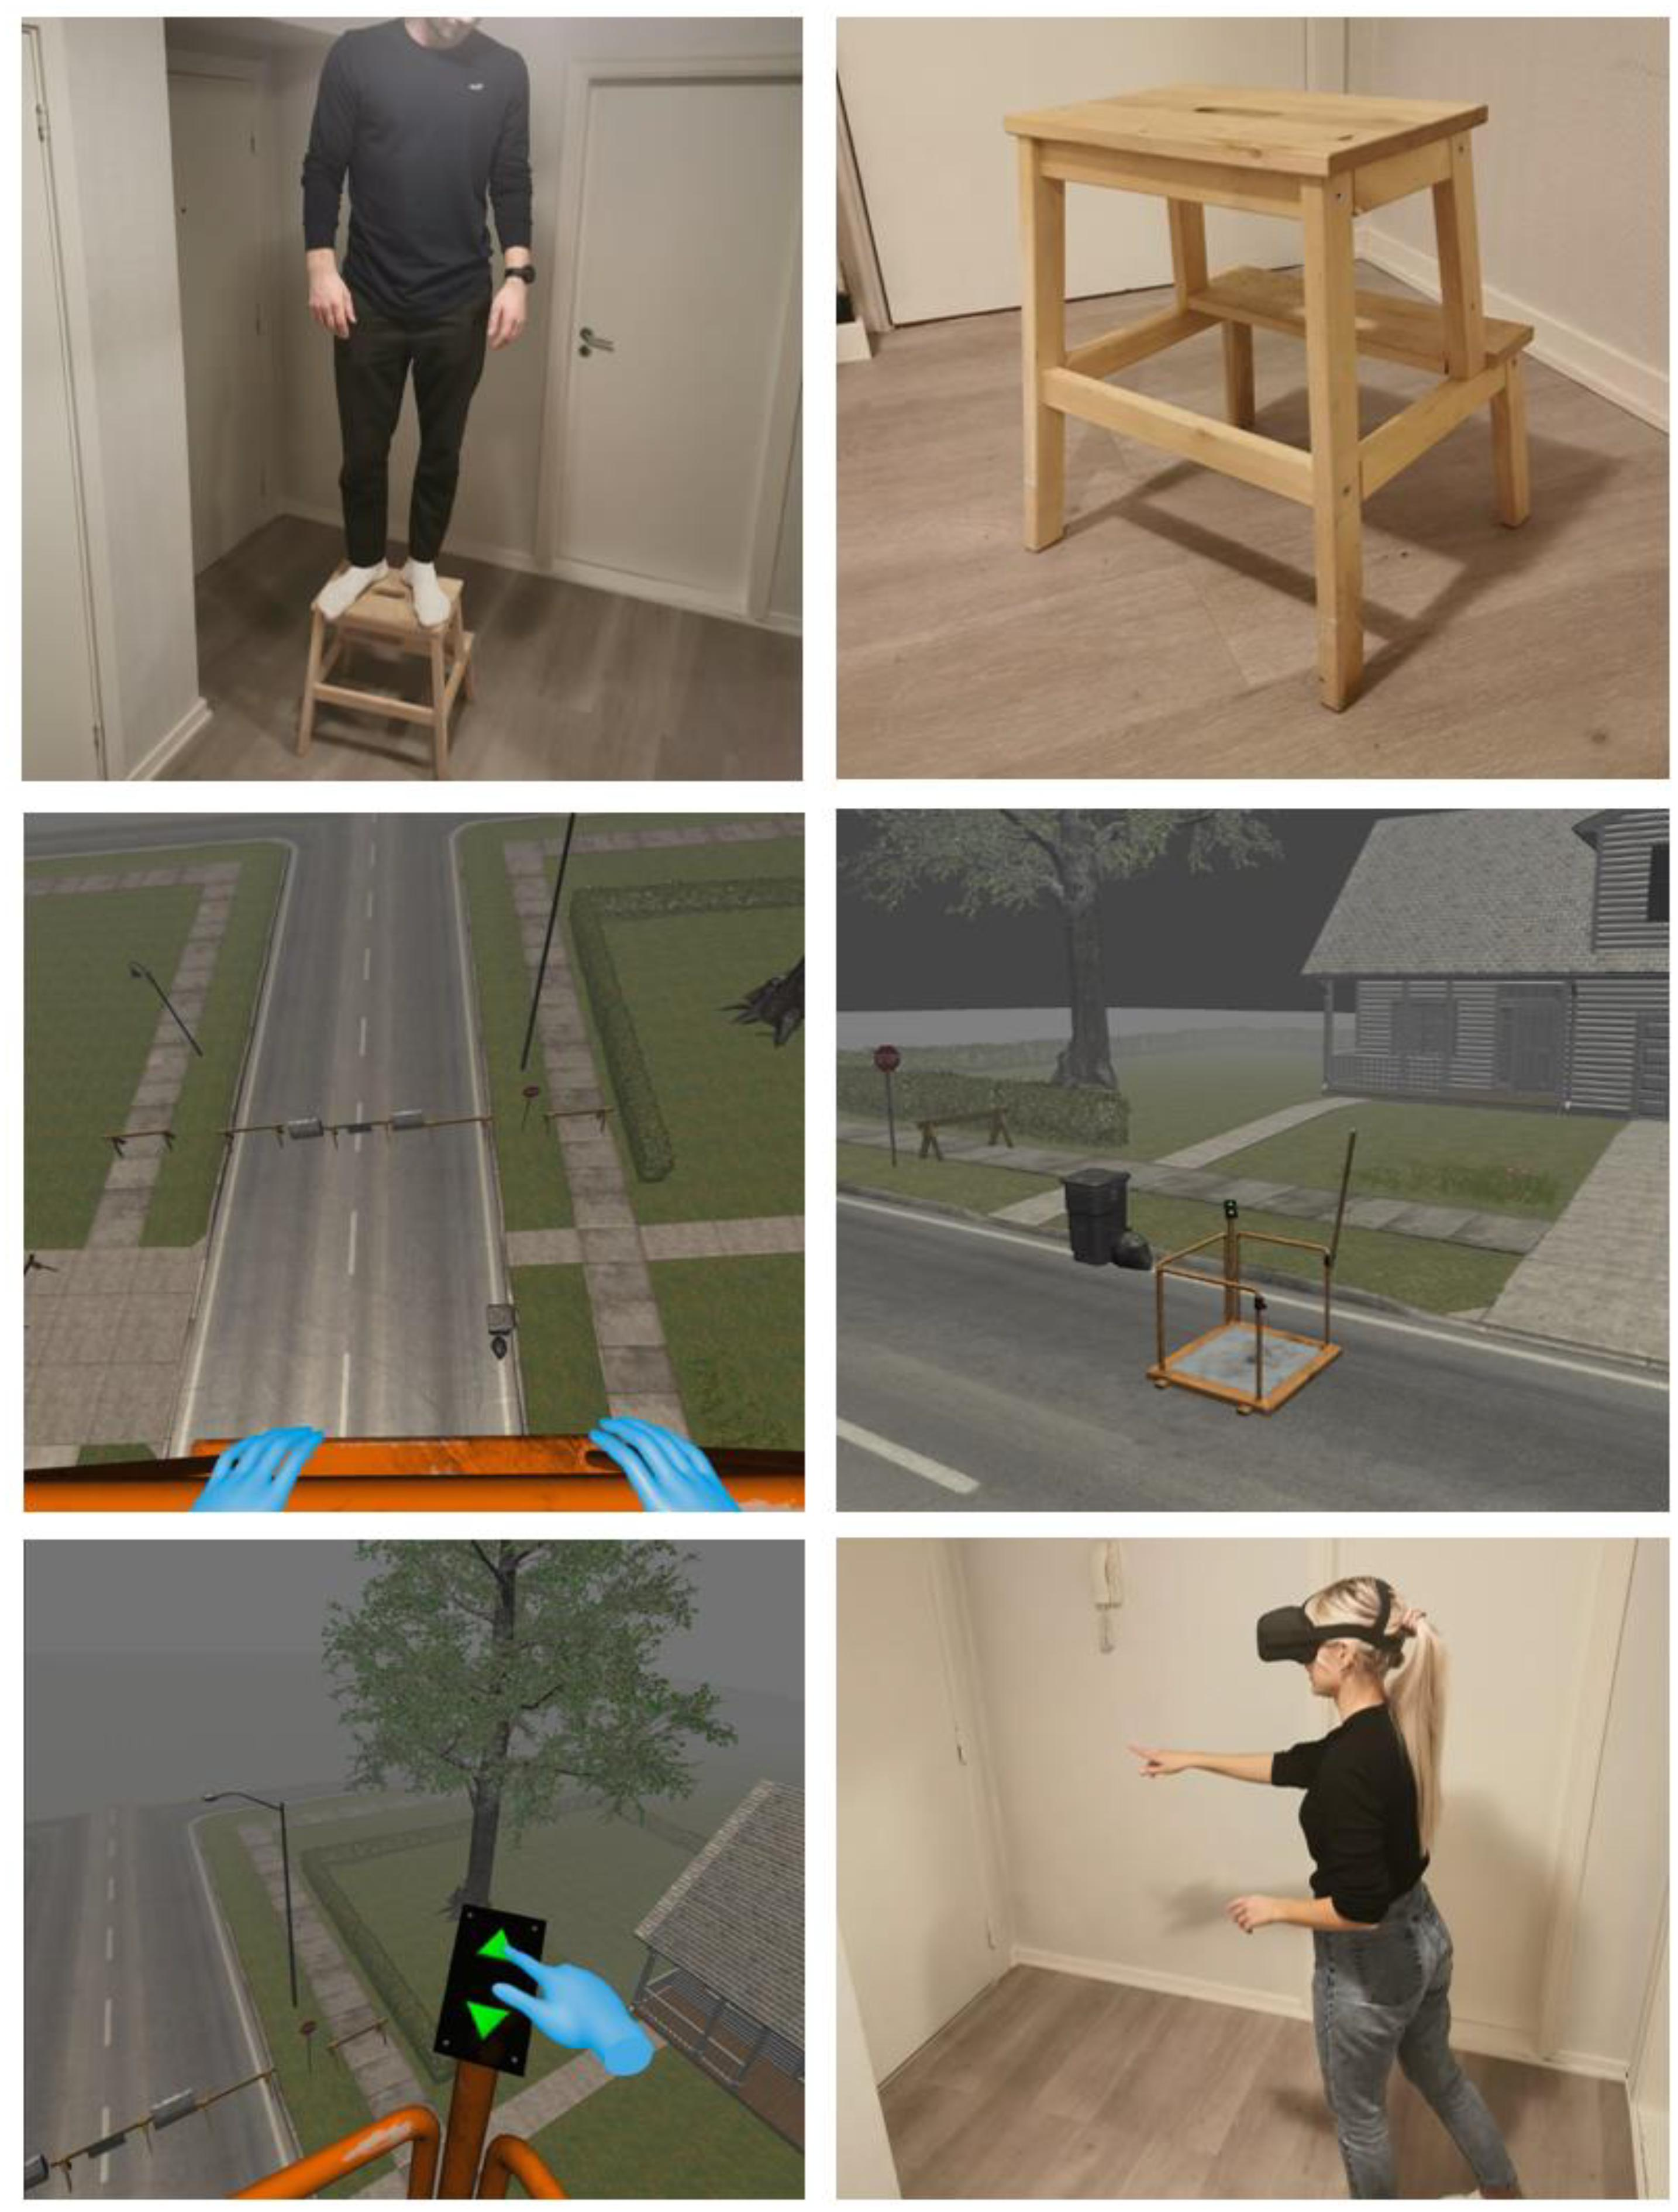
\includegraphics[width=0.6\linewidth]{capitulos/figuras/fear_of_heights.jpg}
    \caption{Exemplo de aplicação que usa \acrshort{RV} no tratamento da acrofobia \cite{Edwards2018}.}
    \label{fig:medoAltura}
\end{figure}

A indústria do entretenimento através de filmes e jogos provocou uma grande evolução de técnicas de \acrshort{RV} que posteriormente foram aplicadas em áreas mais “sérias” como o desenvolvimento pessoal e treinamento \cite{Ma2011, Prensky2001, Smith2011}. Na prática a \acrshort{RV} deve ser considerada como uma possibilidade sempre que o que se deseja fazer é muito perigoso, caro ou impraticável de ser realizado concretamente. Por conta destas características ela é muito usada nas áreas da educação, da saúde e militar \cite{VRS2018}. Conforme a tecnologia que permite a criação e simulação de ambientes virtuais se torna mais barata, mais aplicações são criadas com o uso destas ferramentas.

\section{Dispositivos Hápticos}

O termo \textit{haptics} é usado para descrever a ciência que estuda e simula a pressão, textura, vibração e outras sensações biológicas relacionadas ao toque. A sensação do toque se origina em estímulos mecânicos, elétricos, térmicos ou químicos na pele \cite{Burdea1996}. O tato não está localizado numa região específica do corpo como os demais sentidos. Ele está distribuído por todo o corpo através do órgão sensorial do toque, nossa pele, articulações, músculos e tendões. O senso do toque se divide em duas sensações: cinética e tátil. Forças e torques são sensações cinéticas que sentimos nos músculos, tendões e articulações. Já as sensações táteis como pressão, deformação e vibração são sentidas por mecano receptores que possuímos na nossa pele \cite{Culbertson2018}. 

Os primeiros dispositivos hápticos foram originados dos braços robóticos usados para o controle remoto de robôs \cite{Zurawski2005} As aplicações de tecnologias hápticas são muito variadas envolvendo, por exemplo, projetos de engenharia e aplicações de manufatura \cite{Sharma2001}, entretenimento (videogames e filmes), celulares, relógios inteligentes e até mesmo a indústria automobilística \cite{Smith2019}. Estes dispositivos possuem elementos mecânicos de entrada e saída para interação com o usuário. Uma ou mais partes do dispositivo em contato com o usuário são monitorados no espaço físico e o dispositivo oferece como retorno força e torque. Desta forma um canal bidirecional de interação entre o ambiente virtual e o usuário é criado \cite{Coles2011}. Estes dispositivos estão sendo cada vez mais utilizados hoje em dia tanto pela evolução da sua tecnologia como pela diminuição dos preços. Com o avanço da tecnologia estes dispositivos estão se tornando cada vez mais flexíveis representando mais fielmente os movimentos. Isto ocorre  através do uso de conceitos de restrição parcial a movimentos, deslocamentos e da inclusão de mais graus de liberdade, \textit{\acrfull{DoF}}. 

O número de graus de liberdade de um dispositivo háptico se refere ao número de maneiras diferentes em que este pode se mover ou criar forças. Como exemplo, dispositivos com 3 graus de liberdade podem rastrear posições e criar forças ao serem movidos nas direções: direita-esquerda, frente-trás e cima-baixo \cite{HAPTICSHOUSE2019}. O principal objetivo no uso destes dispositivos é o aumento da sensação de imersão em um ambiente de realidade virtual. 

Em relação à área médica, os dispositivos hápticos vem sendo utilizados na maioria dos trabalhos de simulação de procedimentos médicos \cite{Coles2011,Escobar-Castillejos2016}. Eles são usados para simular o uso de ferramentas em cirurgias e ajudaram a impulsionar o sucesso das práticas em simuladores virtuais. Isto aconteceu ao proporcionar o controle dos graus de liberdade de deslocamentos, a restrição aos movimentos e as respostas às atitudes do usuário como forças de reação ou \textit{feedback} \cite{Gerovich2004}. Estes dispositivos eletromecânicos existem nas mais diversas formas e são adaptados para uma grande variedade de procedimentos médicos como, por exemplo, no treinamento de laparoscopia \cite{Srinivasan2004}, biopsia de próstata \cite{Sclaverano2009}, cirurgia de fígado \cite{Mastmeyer2016}, exames de mama \cite{Brazil2017,Jeon2010,Ribeiro2014,Solanki2010}, simulação de apalpação \cite{Ribeiro2016} e punções epidurais \cite{N.2013, Brazil2018}. Alguns sistemas usam mais de um háptico como em punções de agulha guiadas por ultrassom que usam um equipamento para simular a agulha e outro para o ultrassom \cite{Ni2011,Vidal2008}. Outros chegam a fazer o uso de três dispositivos como o PalpSim de forma a simular o toque das mãos do usuário num paciente virtual \cite{Coles2011b}. 

Culbertson et al. identificaram como 3 as principais categorias de sistemas hápticos: compreensíveis, vestíveis e palpáveis. Um exemplo visual destes tipos pode ser visto na Figura 6. Os sistemas compreensíveis são dispositivos tipicamente cinéticos (\textit{feedback} de força) que normalmente possuem uma base fixa e permitem ao usuário empurrar e ser empurrado de volta. Sistemas vestíveis são tipicamente táteis montados nas mãos ou em outras partes do corpo e provocam sensações diretamente na pele. Os sistemas palpáveis são dispositivos de encontro que permitem ao usuário explorar toda a superfície \cite{Culbertson2018}. Os dispositivos a serem explorados aqui são os de sistemas compreensíveis. Estes foram os tipos de hápticos utilizados nos simuladores computacionais relacionados ao tema desta tese (seção 0) assim com nos diversos outros simuladores médicos estudados e citados nesta seção. Ribeiro et al. fizeram uma revisão sobre dispositivos usados na simulação de procedimentos que envolvem o toque da mão do médico para identificação de características e anormalidades sob a pele \cite{Ribeiro2016}. Os autores analisaram 57 trabalhos e mais da metade fez uso dos dispositivos da família \textit{Phantom}. Os dispositivos desta família serão listados na seção ===== 3 ======.

===== FIGURA ====

Nas figuras Figura 7, Figura 8, Figura 9 e Figura 10 os dispositivos aparecem representados ordenados pelas suas complexidades i.e. dos mais simples (mais antigos e com menos recursos) aos mais avançados (mais novos). Todos estes dispositivos são exemplos de sistemas tipicamente cinéticos. Os mais novos possibilitam maior número de graus de liberdade para os movimentos assim como possibilitam mais forças e momentos de reação. O Novint Falcon ® (Figura 7), lançado em 2007, tem como interface com o usuário uma esfera onde o usuário deve colocar os dedos da mão para fazer os movimentos no caso do seu uso mais comum. No que diz respeito à liberdade de movimento este mecanismo proporciona uma interação 3D com o computador no lugar da interação 2D proporcionada pelo mouse. Ele possui 3 graus de liberdade de movimento e de forças. Nesta esfera existem quatro botões para interação e existem sensores para determinar a posição do cursor e motores para controlar as forças a serem transmitidas para o usuário. Existem versões onde a esfera é substituída, por exemplo, por um dispositivo semelhante a uma pistola para que o dispositivo seja usado em jogos de tiros de primeira pessoa \cite{VRS2017}. 

===== FIGURA ====

Os hápticos da família \textit{Phantom Geomagic Touch} ® (Figura 8) e \textit{Geomagic Touch} X ® (Figura 9) apresentam uma peça que simula uma caneta para manipulação do usuário da mesma forma que a esfera no dispositivo da Figura 7. Nas canetas também existem botões para interação e da mesma forma estas também são substituíveis por partes com formas mais adequadas ao procedimento que estas pretendem simular. O dispositivo \textit{Geomagic Touch} X ® possui a mesma liberdade de movimento do \textit{Geomagic Touch} ®, porém possibilita \textit{feedback} de reações maiores. Ambos apresentam 6 graus de liberdade de movimento e 3 graus de liberdade no retorno de forças. Estes dispositivos, portanto mapeiam a posição 3D e orientação, mas somente apresentam \textit{feedback} de forças direcionais \cite{Forsslund2013}.

===== FIGURA ====

===== FIGURA ====

O \textit{Phantom Premium} ® (Figura 10) está disponível nas versões \textit{Premium} 1.0, \textit{Premium 1.5} e 1.5/HF, e \textit{Premium} 3.0. Estas evoluem não só o \textit{feedback} de reações como também os graus de liberdade dos movimentos. Enquanto o \textit{Phantom Premium} 1.0 ® simula o movimento do giro do pulso na mão o \textit{Phantom Premium} 3.0 ® possibilita uma amplitude que simula os graus de liberdade de movimento de todo o braço humano desde o ombro \cite{3DSystems2018}. Este dispositivo possui 6 graus de liberdade tanto para movimento como retorno de forças o que o torna simétrico no número de sensores e motores (atuadores). São computadas forças e torques tanto da posição como da orientação deste dispositivo. Esta característica tem uma forte influencia no alto custo associado a este tipo de dispositivo \cite{Forsslund2013}.

===== FIGURA ====

=========

\section{Modelagem de tecidos}

Um dos passos necessários para construção de um ambiente virtual para treinamento de anestesia epidural e raquianestesia é a criação de pacientes virtuais. Um importante aspecto da modelagem destes pacientes é como eles aparecem na tela da aplicação. Outro aspecto importante na simulação é ter uma estimativa da espessura dos tecidos envolvidos nestes tipos de anestesia. Para isto é necessária à modelagem do tamanho de todas as camadas de tecido pelos quais as agulhas passam para execução destes procedimentos. Uma ilustração destes tecidos que vão desde a pele até a dura-máter pode ser vista na Figura 3. Nesta seção são descritos trabalhos relacionados com a modelagem da distância entre a pele e a dura-máter.

Na Tabela 2 são listadas as varáveis de entrada e saída dos métodos estudados nesta seção. Esta tabela exibe também as unidades destas variáveis que serão utilizadas em todo este trabalho.

===== TABELA ====

Muitos trabalhos buscam relacionar a distância que vai da superfície externa da pele até o espaço epidural (DEE) com as demais variáveis da Tabela 2. A grande maioria dos trabalhos indica uma forte relação da DEE com o IMC \cite{Adegboye2017, Galbraith2018}. Estes dois trabalhos não fazem separação dos grupos populacionais por idade, sexo ou etnia, e usaram populações respectivamente de n=120 e n=317 pessoas entre homens e mulheres.

Os trabalhos citados a seguir analisaram somente ou de forma separada grupos de mulheres grávidas. Como este é o foco deste trabalho só serão comentadas aqui as conclusões referentes a estes grupos. Todos os trabalhos a seguir encontraram influencia do IMC na determinação da DEE, mas além desta relação também foram encontradas outras combinações em cada trabalho. O grupo étnico/populacional do individuo foi observado em conjunto com o IMC em \cite{Sharma2011} estudo feito no Reino Unido. A idade foi observada em conjunto com o IMC num estudo em pacientes americanas em Michigan, EUA \cite{Clinkscales2007}. A altura, massa, idade e IMC foram observados como relevantes em um estudo em pacientes da Índia \cite{Hazarika2016}. Estes dois últimos trabalhos construíram equações de regressão linear para determinação da DEE para grupos de parturientes conforme pode ser visto na Tabela 3.

===== TABELA ====

Os autores em \cite{Sharma2011} no lugar das equações apresentaram como resultado uma tabela com cinco pontos de cada par IMC x DEE para cada grupo populacional analisado. Estes dados podem ser vistos na Tabela 4. A definição dos grupos populacionais no estudo do Reino Unido (RU) em \cite{Sharma2011} foi: Brancas (população do Reino Unido, da Irlanda e qualquer outro grupo com cor de pele branca); Asiáticas ou Britânicas Asiáticas (população da Índia, Paquistão, Bangladesh ou qualquer outro grupo Asiático); Negras ou Britânicas negras (população de Africanas, Caribenhas ou outros grupos com cor da pele negra); e Chinesas e outros grupos étnicos (população da China, Japão, Malásia, Filipinas etc.). No grupo de nome Chinesas, além dos dados de pessoas desta origem moradoras do Reino Unido, foram considerados dados de Chinesas (n=70) de um hospital de Singapura.

===== TABELA ====

Na Tabela 5 é apresentado o tamanho da população utilizada nestes estudos e as identificações da origem dos dados do estudo, isto é, os grupos populacionais analisados. 

===== TABELA ====

A listagem dos tecidos entre a pele e a DEE e a relação dessa distância com o aumento de peso é comentada em \cite{Palmer1983}. Os autores concluem que com o aumento do peso/massa (do paciente) o tecido que sofre a maior variação é a gordura subcutânea.

Na seção = ==== é proposto o uso de dados de trabalhos comentados aqui para modelagem de tecidos de pacientes grávidas.

=========

Este capítulo apresentou uma fundamentação teórica sobre ====. Iniciou apresentando ==========. Logo em seguida o capítulo apresenta ====== e suas principais entidades e que estão relacionadas com a proposta desta tese. O capitulo finaliza apresentando os conceitos que envolvem ==== e seus principais elementos. O próximo capítulo oferece uma visão das pesquisas relacionadas ao tema desta tese e compara-as com as proposições que foram colocadas ao longo deste trabalho. Essas pesquisas tratam e ========== assim como de ===========.  %inclui novo capítulo

\pagestyle{ruledheader}
\chapter{Trabalhos Relacionados} \label{cap:cap3}

%Os trabalhos apresentados neste capítulo vão desde simuladores que usam só \texit{phantoms} a simuladores computacionais. É interessante destacar que alguns simuladores computacionais são híbridos no sentido de que usam \textit{phantoms} como parte do processo de simulação. 

Os trabalhos apresentados neste capítulo vão desde abordagens de simulação de procedimentos de anestesia usando \textit{phantons} passando por simuladores computacionais bem como os diferentes tipos de modelagens de partes do corpo humano usados para simulações médicas.  

\textcite{Vaughan2013} citam trinta e um simuladores (entre computacionais e com uso de \texit{phantoms}). Destes, dezesseis são apenas epidurais, nove que permitem tanto a punção epidural quanto a raquidiana e seis apenas raquidianos. São discutidas as limitações e vantagens de cada um, de forma a identificar características desejáveis para serem incluídas em um simulador \cite{Vaughan2013}. No trabalho de \textcite{Isaacs2015} os autores citam uma pesquisa onde também são elencadas diversas características interessantes para um simulador epidural \cite{Isaacs2015}. Dentre os itens com mais relevância citados por \textcite{Isaacs2015} estão: coluna fisicamente palpável, representação da técnica de perda de resistência (do inglês inglês Lost of Resistence, \acrshort{LOR}) de forma realista (para solução salina e ar), ajuste da posição do paciente, mapeamento de características do paciente (obesidade, gravidez), \texit{feedback} a respeito da correta execução.
A principal vantagem dos modelos com uso de \texit{phantoms} é a presença física do manequim que representa o paciente. Uma das principais desvantagens é a dificuldade na variabilidade de cenários (pacientes) distintos. Outra desvantagem é a dificuldade na representação da diferença existente entre a resistência dos tecidos biológicos e os tecidos nos quais os modelos físicos são constituídos (usualmente borracha e plástico).
Os dispositivos hápticos têm melhorado muito ao longo dos últimos anos. Os modelos computacionais com hápticos têm como pontos a favor a versatilidade. As possibilidades computacionais da tecnologia háptica e as visualizações 3D de tempo real são outros pontos positivos associados a esta tecnologia. 
Soluções computacionais podem criar um modelo de forças de inserção da agulha. Para este fim pode-se usar como base as medições das forças aplicadas para inserção de agulhas em animais considerados próximos dos humanos, assim como em cadáveres e até mesmo voluntários reais \cite{Hiemenz1998, Holton2001,Langton1990,McKay2010,Naemura2009,Tran2009,Vaughan2012}. Estes modelos podem contemplar uma grande variabilidade de cenários através de ajustes de parâmetros. 

A seguir serão apresentados os simuladores de punções mais completos. Primeiro os que somente fazem uso de \textit{phantoms}, em seguida os que usam de ferramentas computacionais.  

\section{Simuladores que só usam \texit{phantoms}} \label{sec:SimuladoresPhantoms}

Os simuladores baseados em \texit{phantoms} (ou manequins) mais completos são listados aqui com suas principais características. As características positivas devem idealmente ser contempladas ou até melhoradas em novos simuladores. Todas as soluções listadas estão disponíveis atualmente. Elas permitem ao menos a simulação da anestesia peridural, possuem a coluna fisicamente palpável e permitem a escolha do ponto e ângulo de inserção da agulha. Todos esses trabalhos permitem que o procedimento seja feito com o paciente sentado ou deitado e o escoamento do fluido cérebro espinhal é simulado ao perfurar a dura-máter. As abordagens mediana e paramediana de inserção de agulha são possíveis em todos estes simuladores.

A solução \texit{SimULab Lumbar Epidural Trainer} possui até 3 variações de pacientes (normal, idoso e obeso). A Figura \ref{fig:simuladorSimulab} ilustra o uso deste simulador onde na esquerda da imagem (a) está a simulação da inserção da agulha no manequim e na imagem da direita (b) o uso do ultrassom. O material deste manequim foi produzido de forma a permitir o uso de ultrassom \cite{SimulabCorporation2008}. 

\begin{figure}[ht!]
    \centering
        \begin{tabular}{cc}
        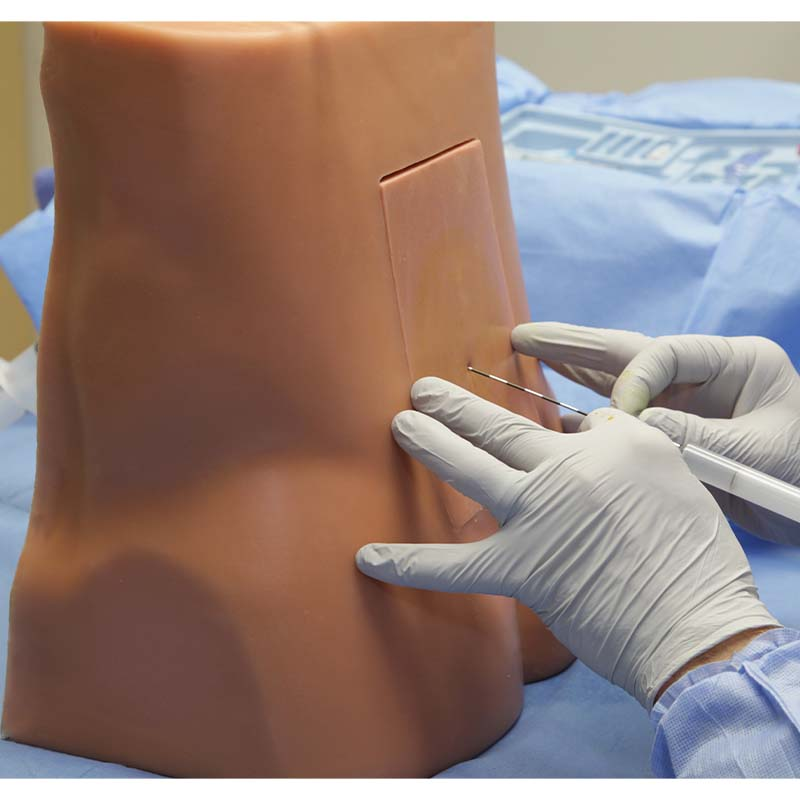
\includegraphics[width=0.3\linewidth]{capitulos/figuras/simulab-insercao-agulha.jpg} & 
        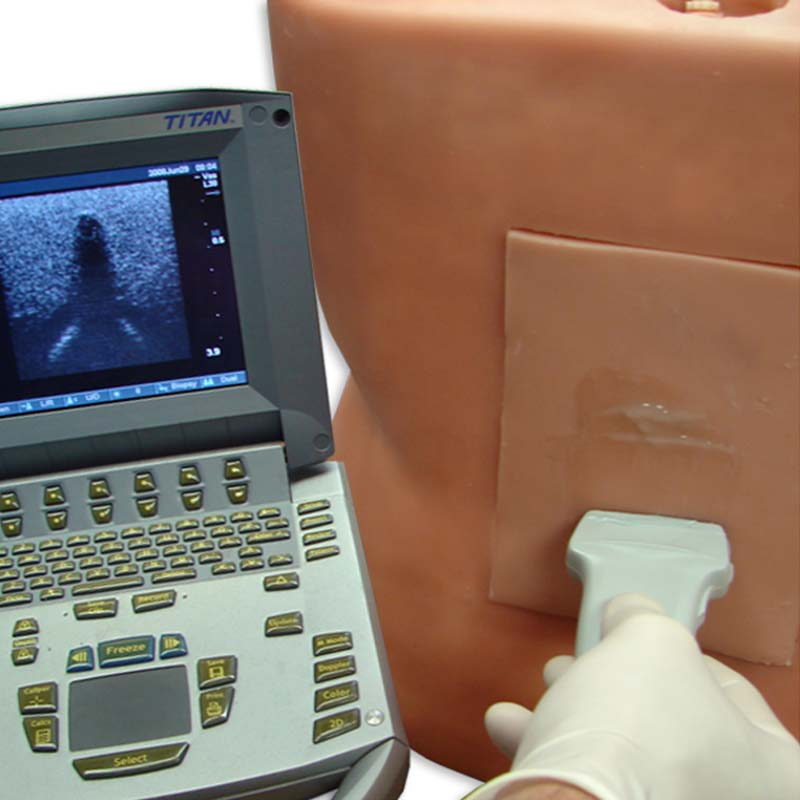
\includegraphics[width=0.3\linewidth]{capitulos/figuras/simulab-ultrassom.jpg} 
        \\
        (a) & (b)
        \end{tabular}
    \caption{Demonstração de uso do simulador SimULab Lumbar Epidural Trainer \cite{SimulabCorporation2008}.}
    \label{fig:simuladorSimulab}
\end{figure}

O \textit{Blue Phantom Lumbar Puncture and Spinal Epidural} (Figura \ref{fig:bluePhantom}) também foi produzido em material que possibilita o uso do ultrassom. Na imagem (a) aparece o manequim e na (b) e (c) aparecem respectivamente o uso do ultrassom e o escorrimento do líquor. Este simulador possui somente duas opções de variação de pacientes (normal e obeso) \cite{BluePhantom2011}. 

\begin{figure}[ht!]
    \centering
        \begin{tabular}{ccc}
        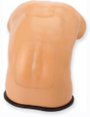
\includegraphics[width=0.17\linewidth]{capitulos/figuras/BluePhatom-manequim.png} & 
        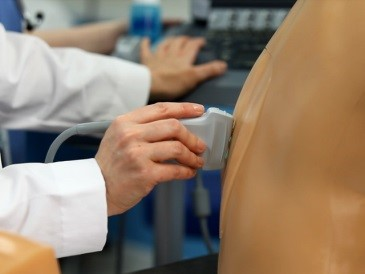
\includegraphics[width=0.3\linewidth]{capitulos/figuras/BluePhatom-ultrassom.jpg} 
        &
        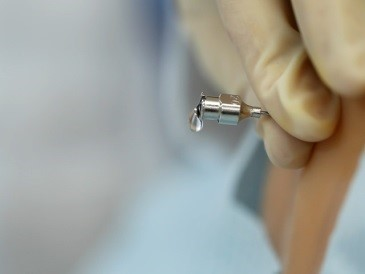
\includegraphics[width=0.3\linewidth]{capitulos/figuras/BluePhatom-escorrimentoLiquor.jpg} 
        \\
        (a) & (b) & (c)
        \end{tabular}
    \caption{Blue Phantom Lumbar Puncture and Spinal Epidural \cite{BluePhantom2011}.}
    \label{fig:bluePhantom}
\end{figure}

O M43B \textit{Lumbar puncture simulator}-II (Figura \ref{fig:m43bSimulator}) permite 3 variações de pacientes (normal, idoso e obeso) e simula também a anestesia raquidiana \cite{KyotokagakuCo.2011}. Uma limitação deste é somente apresentar as vértebras L2 até L5 mas como vimos anteriormente, na seção \ref{sec:anestesiaRaquidiana}, estas são as vértebras mais comuns para anestesia raquidiana. A imagem apresenta o kit completo à esquerda, a palpação da coluna no centro e a inserção da agulha à direita.

\begin{figure}[ht!]
    \centering
        \begin{tabular}{ccc}
        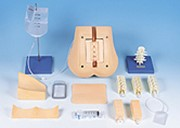
\includegraphics[width=0.3\linewidth]{capitulos/figuras/m43b-kit.jpg} & 
        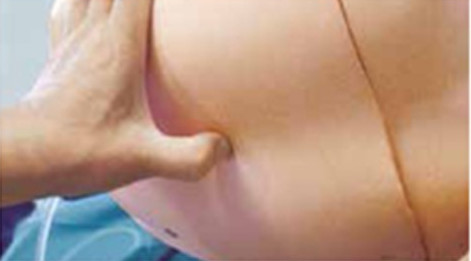
\includegraphics[width=0.3\linewidth]{capitulos/figuras/m43b-usoPalpacao.jpg} 
        &
        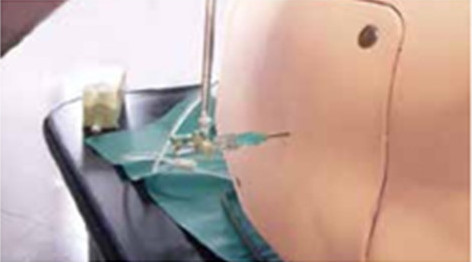
\includegraphics[width=0.3\linewidth]{capitulos/figuras/m43b-usoAgulha.jpg} 
        \\
        (a) & (b) & (c)
        \end{tabular}
    \caption{Kit e exemplo de uso do simulador M43B \texit{Lumbar puncture simulator}-II \cite{KyotokagakuCo.2011}.}
    \label{fig:m43bSimulator}
\end{figure}

Outro simulador que também permite a anestesia raquidiana é o \texit{Nasco Life/form® Spinal Injection Sim}. As vértebras L1 e L2 ficam visíveis externas ao corpo simulado pelo manequim. Ele somente permite a punção entre as vértebras L3 até L5 \cite{Nasco2008}. Na imagem da Figura \ref{fig:nascoSimulator} aparece um exemplo de uso deste simulador.

\begin{figure}[ht!]
    \centering
    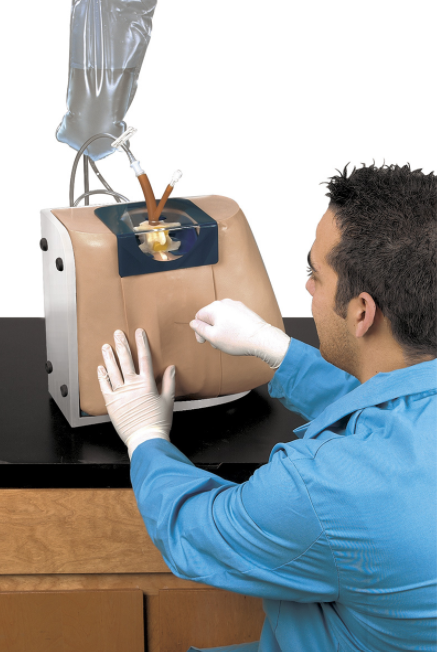
\includegraphics[width=0.3\linewidth]{capitulos/figuras/nascoSimulator.png} 
    \caption{Demonstração de uso do simulador \textit{Nasco Life/form® Spinal Injection Sim} \cite{Nasco2008}.}
    \label{fig:nascoSimulator}
\end{figure}

A Tabela \ref{tab:comparacaoSimuladoresPhantoms} resume uma série de características importantes destes simuladores. 

\begin{table}[!ht]
\begin{center}
\caption{Comparação dos simuladores epidurais baseados em phantoms.}
\label{tab:comparacaoSimuladoresPhantoms}
%\begin{tabular}{|p{0.27\linewidth}|p{0.55\linewidth}|p{0.105\linewidth}|}
\begin{tabular}{|c|c|c|c|c|c|c|c|c|}
\hline
  & 
  \rotatebox{90}{Ano de desenvolvimento} & 
  \rotatebox{90}{Epidural (E) Raquianestesia (R)} & 
  \rotatebox{90}{Testado em hospital} & 
  \rotatebox{90}{Permite o uso de ultrassom} & 
  \rotatebox{90}{Variabilidade de pacientes} & 
  \rotatebox{90}{Coluna palpável} & 
  \rotatebox{90}{Escolha do ponto de inserção da agulha }  & 
  \rotatebox{90}{Abordagens mediana e paramediana} \\
\hline\hline
 SimULab Lumbar Epidural Trainer & 2008 & E &  & OK & 3 & OK & OK & OK \\
 {\begin{tabular}[c]{@{}c@{}}Blue Phantom Lumbar Puncture\\ and Spinal Epidural\end{tabular}} & 2011 & ER &  & OK & 2 & OK & OK & OK \\
 M43B Lumbar puncture simulator-II & 2010 & ER & OK &  & 3 & OK & OK & OK \\
 Nasco Life/form® Spinal Injection Sim & 2008 & ER &  &  & 3 & OK & OK & OK \\
\hline
\end{tabular}
\end{center}
\end{table}

\section {Simuladores computacionais}

Esta seção comenta os simuladores computacionais que possuem as características mais relevantes ao desenvolvimento pretendido.

O primeiro simulador epidural computacional, Epidural Sim \cite{Stredney1996} apresentou uma série de características interessantes. A representação do corpo do paciente em 3D teve a variabilidade de seus elementos obtida através de exames de \acrfull{RM}. Permite o uso de uma agulha real ligada a um dispositivo háptico. O modelo de forças foi baseado em medidas feitas durante inserções epidurais em porcos e cães combinados com opiniões de especialistas. Este simulador permite ainda a escolha do ponto de inserção da agulha assim como o seu ângulo. É disponibilizada uma interface de voz, o que possibilitava ser iniciado por comandos de voz do usuário assim como receber \texit{feedbacks} gerados pelo computador. A palpação da coluna não está disponível neste simulador. Chegou a ser testado por anestesistas que o consideraram muito mecânico, porém com potencial de melhora a partir de ajustes. Uma imagem do uso deste simulador pode ser vista na Figura \ref{fig:epiduralSim}. 

\begin{figure}[ht!]
    \centering
    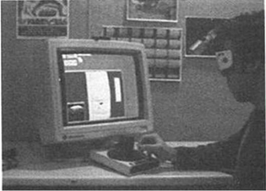
\includegraphics[width=0.3\linewidth]{capitulos/figuras/epiduralSimulator.png} 
    \caption{Epidural Sim em uso \cite{Stredney1996}.}
    \label{fig:epiduralSim}
\end{figure}

O único simulador computacional estudado que possibilita a palpação da coluna é o \texit{Epidural Injection Simulator, EIS} \cite{Wilson2003}. Esta característica é atendida através de um equipamento físico que fica conectado a uma unidade de controle. O simulador possui uma interface gráfica que mostra, em tempo real, a progressão da agulha em cada camada de tecido conforme ela é inserida. Existem 6 variações de pacientes e um \texit{feedback} de forças configurável. Não permite a escolha do ponto de inserção da agulha nem o seu ângulo de inserção, que são fixos. Uma nova versão deste simulador foi desenvolvida com o nome de \texit{Epidural Injection Simulator Profile Manager}. Essa, além das funcionalidades do seu antecessor possibilita a criação de cenários customizados de pacientes além das 6 opções pré-configuradas. Estas customizações podem inclusive ser salvas para uso posterior. O \texit{feedback} em tempo real nesta nova versão pode ser visualizada no monitor do computador no lugar da unidade de controle \cite{CPRSavers&FirstAidSupply2018}. A Figura \ref{fig:EpiduralInjectionSimulator} exibe o visual do \texit{Epidural Injection Simulator Profile Manager} e do seu antecessor EIS que foi descontinuado com o lançamento da nova versão.

\begin{figure}[ht!]
    \centering
        \begin{tabular}{cc}
        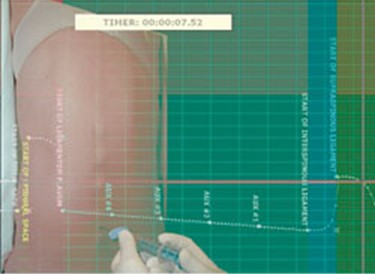
\includegraphics[width=0.4\linewidth]{capitulos/figuras/epiduralInjectionSimulatorPM.jpg} & 
        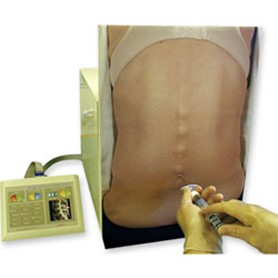
\includegraphics[width=0.3\linewidth]{capitulos/figuras/epiduralInjectionSimulator.jpg} 
        \\
        (a) & (b)
        \end{tabular}
    \caption{Imagens de exemplo das duas versões do \texit{Epidural Injection Simulator}: (a) \texit{Versão mais nova: Profile Manager} (b) Versão antiga: EIS (descontinuado)  \cite{CPRSavers&FirstAidSupply2018}.}
    \label{fig:EpiduralInjectionSimulator}
\end{figure}

Em 2006 foi lançado o \textit{Mediseus® epidural simulator} (MedicVision Pty Ltd, Melbourne, Austrália). Este simulador apesar de ter sido descontinuado apresentava algumas características interessantes como a exibição completa do corpo permitindo rotações e zoom \cite{Mayooran2006}. A pele pode ser tornada transparente tornando visíveis as cinco vértebras modeladas. Este simulador usa um \textit{Phantom Omni} dentro de uma caixa patenteada \cite{Brien2007} para o \textit{feedback} das forças na agulha incluindo a medida da pressão de ar na seringa. A agulha é movida na tela em tempo real assim que o dispositivo é movimentado. O dispositivo pode ser conectado em qualquer laptop. Em uma avaliação feita sobre este simulador de 2007 \cite{Elks2007} ele não teve um bom retorno por parte dos anestesistas. O item com pior avaliação foi a sensação de LOR que somente 54\% dos especialistas julgaram como realista. Em um estudo posterior \cite{Lee2012} essa técnica foi avaliada com nota 4,7 de um valor máximo de 5 o que supõe uma representação próxima da sensação real esperada. Uma imagem deste simulador pode ser vista na Figura \ref{fig:mediseusSimulator}.

\begin{figure}[ht!]
    \centering
    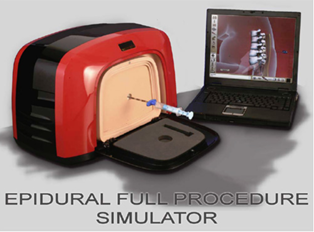
\includegraphics[width=0.6\linewidth]{capitulos/figuras/mediseusSimulator.png} 
    \caption{Aparelho e visual do \textit{Mediseus® epidural simulator}  \cite{Mayooran2006}.}
    \label{fig:mediseusSimulator}
\end{figure}

O \textit{Spinal Anaesthesia Simulator} \cite{Albert2007,Dreifaldt2006}, faz o uso de um dispositivo háptico em conjunto com óculos 3D (Figura \ref{fig:spinalAnestesiaSim}). Permite tanto a simulação da anestesia peridural como a raquidiana. O modelo das costas é feito a partir de uma combinação de imagens de \acrfull{TC} e de \acrshort{RM}. Existem vários níveis de dificuldade configuráveis além de ser possível alterar o nível de visibilidade da pele. Faz uma análise do conhecimento proporcionando um \textit{feedback} ao usuário do nível de aprendizado e as habilidades adquiridas nos vários níveis de dificuldade disponíveis.

\begin{figure}[ht!]
    \centering
    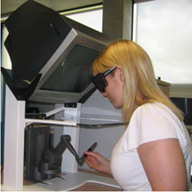
\includegraphics[width=0.3\linewidth]{capitulos/figuras/spinalAnestesiaSim.png} 
    \caption{Forma de uso do \textit{Spinal Anaesthesia Simulator}  \cite{Dreifaldt2006}.}
    \label{fig:spinalAnestesiaSim}
\end{figure}

O EpiSim \cite{YantricInc2011} foi desenvolvido em 2008. Ele faz uso do háptico \textit{Phantom Premium} 1.0 além de um manequim e agulha epidural com uma seringa para recriar a sensação de perda de resistência. A espessura de cada camada de tecido é configurável a partir da interface podendo estas configurações serem salvas para uso futuro. É dado um \textit{feedback} visual a partir de cores, a cor verde indicando o tecido atual e a vermelha indica possíveis toques no osso. Um som de aviso é ouvido no caso de perfuração da dura-máter. É possível efetuar a gravação da inserção de uma agulha inclusive com as forças empregadas para posterior exibição. Esta etapa permite que um procedimento feito por especialistas seja visualizado em detalhes por profissionais inexperientes. A Figura \ref{fig:epiSim} ilustra este simulador.

\begin{figure}[ht!]
    \centering
    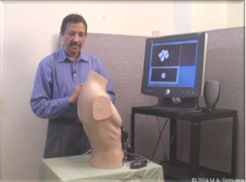
\includegraphics[width=0.4\linewidth]{capitulos/figuras/epiSim.png} 
    \caption{Imagem do simulador \textit{EpiSim} \cite{Frazzetto2011}.}
    \label{fig:epiSim}
\end{figure}

Um simulador de punção lombar criado por \textcite{Farber2008}  possui além do dispositivo háptico \textit{Phantom Premium} 1.0, gráficos anatômicos e tela estereográfica. Os movimentos de rotação e transversais são restritos quando a agulha está dentro do corpo. As forças hápticas são calculadas a partir de dados segmentados e tomografias \cite{Farber2008, Farber2009}. Uma abordagem de processamento de volume háptico \cite{Lundin2005} foi adaptada pelos autores para mapear as tomografias em forças, este método usa os vetores gradientes das imagens para este fim. O paciente virtual 3D é construído a partir de dados de tomografia de pacientes reais e de dados do projeto \textit{Visible Human}. As visualizações incluem uma anatomia 3D e 3 visualizações 2D mostrando os cortes ortogonais (transversal, frontal e sagital). É possível usar uma visão sob a perspectiva da agulha virtual. A Figura \ref{fig:farberSimVisual} ilustra as opções de visualizações citadas, a visão da agulha aparece na parte superior esquerda. A visão pode ser rotacionada e amplificada por meio de zoom. Possui uma boa impressão de profundidade no corpo virtual através da visão estéreo. Possibilita a variação entre 3 opções de pacientes virtuais. Pelas diversas tecnologias envolvidas este simulador tem um custo consideravelmente maior que os demais. Na Figura \ref{fig:farberSimDispositivos} é possível visualizar os dispositivos envolvidos no uso do simulador. Testes num estudo piloto demonstraram que os médicos treinados neste simulador se saíram melhor do que os que não tiveram acesso a ele \cite{Farber2009}. Para estes testes foi utilizada uma população de n=42 dividida em dois grupos de 21.

\begin{figure}[ht!]
    \centering
    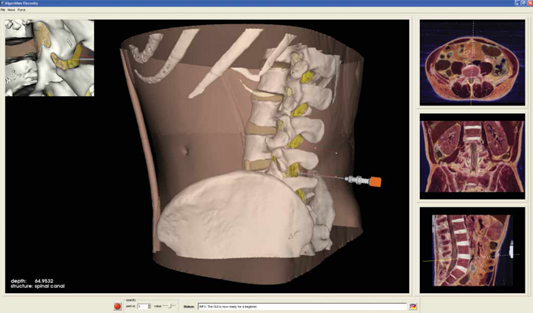
\includegraphics[width=0.8\linewidth]{capitulos/figuras/farberSimVisual.png} 
    \caption{Interface do simulador \cite{Farber2009} com opções de visualização 2D e 3D disponíveis.}
    \label{fig:farberSimVisual}
\end{figure}

\begin{figure}[ht!]
    \centering
    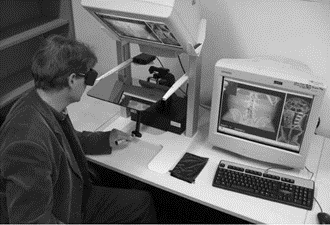
\includegraphics[width=0.5\linewidth]{capitulos/figuras/farberSimDispositivos.png} 
    \caption{Uso do simulador \cite{Farber2009} demonstrando os dispositivos utilizados.}
    \label{fig:farberSimDispositivos}
\end{figure}

O \textit{Epidural Haptic Game Simulator}, EHGS \cite{Brazil2017}, fez uso de dispositivo háptico e elementos de jogos para trazer mais motivação para os usuários. Dentre os elementos de jogos estão presentes a divisão de etapas e atribuição de pontuação pelo correto cumprimento destas no procedimento de punção epidural. A simulação da técnica de LOR foi feita através da exibição de valores na tela ao clicar sobre um botão do háptico simulando o pressionamento do êmbolo da seringa. É possível escolher o ponto e ângulo de inserção da agulha. Não existe a opção de palpação da coluna para descoberta do local correto para efetuação da punção. Foi implementado um modelo de cálculo da espessura dos tecidos conforme peso, altura e idade do paciente de acordo com estudos em parturientes. A modelagem de forças de rigidez, atrito e corte necessárias para inserção e progresso da agulha nos tecidos foi desenvolvida com base em estudos destas forças para inserção de agulhas em tecidos de porcos e humanos. A ferramenta também disponibiliza uma forma manual de alteração destes parâmetros permitindo assim uma customização destas forças segundo as sensações do especialista. A Figura \ref{fig:brasilSimulator} mostra a interface do simulador EHGS em detalhes com o retorno de pontos obtidos, o tecido sendo perfurado no momento, a profundidade da ponta da agulha, as forças medidas e ângulo da agulha.

\begin{figure}[ht!]
    \centering
    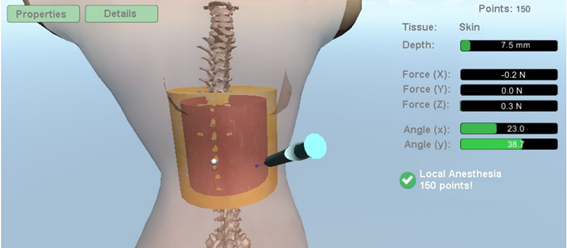
\includegraphics[width=0.8\linewidth]{capitulos/figuras/brasilSimulator.png} 
    \caption{Interface do simulador EHGS \cite{Brazil2017}.}
    \label{fig:brasilSimulator}
\end{figure}

Um resumo das características importantes nos simuladores epidurais computacionais pode ser vista na Tabela \ref{tab:comparacaoSimuladoresComputacionais}.

\begin{sidewaystable}[!ht]
\begin{center}
\caption{Comparação dos simuladores computacionais.}
\label{tab:comparacaoSimuladoresComputacionais}
%\begin{tabular}{|p{0.27\linewidth}|p{0.55\linewidth}|p{0.105\linewidth}|}
\begin{tabular}{|c|c|c|c|c|c|c|c|c|c|c|c|}
\hline
  & 
  \rotatebox{90}{Ano de desenvolvimento} & 
  \rotatebox{90}{Realidade virtual} & 
  \rotatebox{90}{Epidural (E) Raquianestesia (R)} & 
  \rotatebox{90}{Feedback de forças} & 
  \rotatebox{90}{Testado em hospital} & 
  \rotatebox{90}{Baseado em dados medidos} & 
  \rotatebox{90}{Variabilidade de pacientes} & 
  \rotatebox{90}{Feedback para o usuário} & 
  \rotatebox{90}{Coluna palpável} & 
  \rotatebox{90}{Escolha do ponto de inserção da agulha }  & 
  \rotatebox{90}{Abordagens mediana e paramediana} \\
\hline\hline
 Epidural Sim & 1995 & 3D & E & Sim & OK & {\begin{tabular}[c]{@{}c@{}}Porcos e\\cães\end{tabular}} & Múltiplas &  &  & OK & OK \\
 {\begin{tabular}[c]{@{}c@{}}Epidural Injection \\Simulator Profile \\Manager\end{tabular}} & {\begin{tabular}[c]{@{}c@{}}2003\\(1a\\versão)\end{tabular}} &  & E & Customizado &  &  & {\begin{tabular}[c]{@{}c@{}}Múltiplas + salvar \\para uso posterior\end{tabular}} & {\begin{tabular}[c]{@{}c@{}}Habilidade \\rápida; Gráficos\end{tabular}} & OK & &  \\
 {\begin{tabular}[c]{@{}c@{}}Mediseus® epidural \\simulator\end{tabular}} & 2006 & 3D & E & Customizado & OK &  & 2 &  &  & &  \\
 {\begin{tabular}[c]{@{}c@{}}Spinal Anaesthesia \\simulator\end{tabular}} & 2006 & 3D & ER & Phantom &  & TC + RM &  & {\begin{tabular}[c]{@{}c@{}}Conhecimento\\dos níveis de\\dificuldade\end{tabular}} &  & OK & OK  \\
 EpiSim & 2008 & 3D & E & Phantom &  &  & {\begin{tabular}[c]{@{}c@{}}Múltiplas + salvar\\para uso posterior\end{tabular}} & Gravações &  & & OK \\
 {\begin{tabular}[c]{@{}c@{}}Simulador de punção  \\lombar de Färber\end{tabular}} & 2009 & 3D & ER & Phantom & OK & TC & 3 & Gravações &  & OK & OK \\
 EHGS & 2017 & 3D & E & Phantom &  & {\begin{tabular}[c]{@{}c@{}}Porcos e\\humanos\end{tabular}} & Múltiplas & Pontuações &  & OK & OK \\
\hline
\end{tabular}
\end{center}
\end{sidewaystable}

\subsection {Comparação}

Enquanto os simuladores baseados em \textit{phantoms} mais generalistas possibilitam 3 variações de pacientes alguns dos simuladores computacionais mais completos possibilitam infinitas representações de pacientes através de ajustes de parâmetros. Em contrapartida apenas um dos simuladores computacionais desenvolvidos tratou a apalpação física da coluna. Esta é uma característica desejável e importante que está presente em todos os simuladores baseados em \textit{phantoms}. Outra característica muito importante presente na maioria dos modelos baseados em \textit{phantoms} é a escolha do ponto de inserção da agulha e sua angulação. Este fator já está incorporado nos principais simuladores computacionais.

=== CONTINUA ===  %inclui novo capítulo

\pagestyle{ruledheader}
\chapter{Proposta} \label{cap:cap4}

A proposta de uso do dispositivo háptico para treinamento de anestesia raquidiana apresentada nesta tese envolve a criação de um simulador que permite o treinamento de aprendizes na técnica de anestesia raquidiana utilizando um ambiente virtual de treinamento.
Este ambiente virtual foi desenvolvido utilizando o motor de jogo Unity3D \cite{UnityTechnologies2020} com uso de \textit{plugin} para o dispositivo háptico \textit{Geomagic Touch}®, os \textit{scripts} foram desenvolvidos em C\#. O código foi desenvolvido como uma evolução do simulador epidural desenvolvido por \textcite{Brazil2017} levando em consideração que diversas funcionalidades existentes foram estendidas e modificadas. O foco passou de anestesia epidural para anestesia raquidiana. Um novo modelo 3D foi construído para representar fielmente as camadas do corpo humano, para isto as formas e volumes das camadas foram baseadas num corpo 3D interativo cientificamente preciso \cite{BioDigitalInc2019}. Adicionalmente a isto as principais camadas (tecidos do corpo) foram programadas com um margem de crescimento individual onde o crescimento da camada mais interna "empurra" as camadas mais externas pra fora. Isto foi feito para possibilitar uma maior variabilidade de cenários e para que estes sejam visualmente coerentes quando a transparência das camadas for aplicada. Além da possibilidade de se crescer individualmente cada camada, também é possível que todas as camadas cresçam de forma homogênea através da aplicação de matrizes de transformação. 

\section {Desenvolvimento do ambiente de treinamento} 

O modelo 3D para o tronco do corpo feminino (área onde é feita a punção) foi desenvolvido usando o software de modelagem e criação \textit{3ds Max} \cite{Autodesk}. Exemplos das suas diversas camadas internas podem ser observados na figura \ref{fig:modelo3Dcorpo}. 

\begin{figure}[ht!]
    \centering
        \begin{tabular}{cc}
        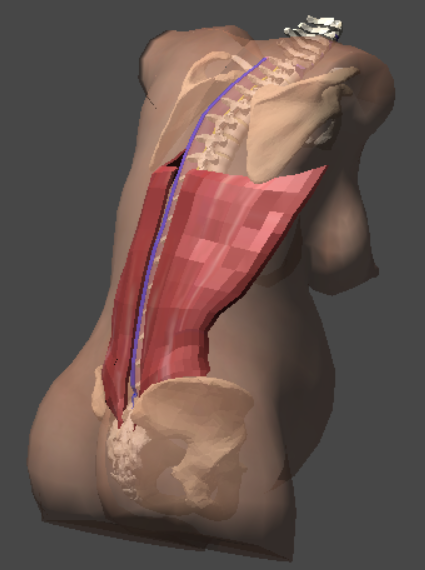
\includegraphics[width=0.4\linewidth]{capitulos/figuras/modelo corpo 3d.PNG} & 
        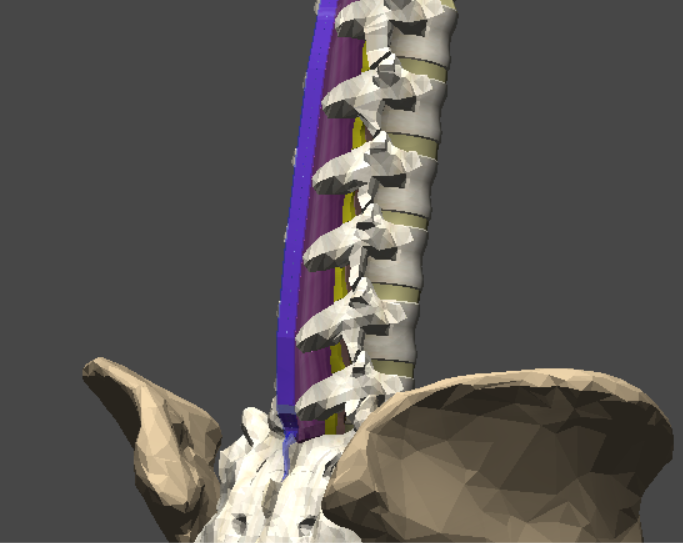
\includegraphics[width=0.6\linewidth]{capitulos/figuras/modelo corpo 3d - coluna vertebral, ligamentos supra, interespinhoso and flavum.PNG} 
        \\
        (a) & (b)
        \end{tabular}
    \caption{Modelo 3D de corpo de mulher grávida desenvolvido com diferentes níveis de transparência \cite{Melo2021}: (a) Corpo, ossos e músculos (b) Osso, vértebras e ligamentos.}
    \label{fig:modelo3Dcorpo}
\end{figure}

Como comentado anteriormente foram criados controles para crescimento das principais camadas do corpo. Primeiro é necessário iniciar um projeto na \textit{Unity} e importar o modelo 3D. Com isto estes controles ficam acessíveis via código nas diversas linguagens suportadas pela \textit{Unity} assim como via interface da \textit{Unity}. Para a nossa solução onde precisávamos fazer modificações em tempo de execução optamos pelo acesso através do código em C# para fazer as modificações de tamanho das camadas (quando necessário). 

Para que seja possível fazer a interação com o dispositivo háptico \textit{Geomagic Touch®} o driver \textit{Open Haptics Touch Device} precisa ser instalado na máquina onde o dispositivo será usado, este driver pode ser encontrado no endereço eletrônico da empresa responsável pela produção e comercialização deste dispositivo háptico \cite{3DSystemsTouch2018}. Para que este dispositivo possa ser utilizado na \textit{Unity} optamos pela instalação do \textit{Haptic Plug-In For Unity3D} \cite{Poyade2014}. Este \textit{plugin} contém exemplos que exploram as funcionalidades e dos dispositivos hápticos suportados. As características específicas que foram utilizadas nos experimentos são comentadas no capítulo~\ref{cap:cap5}. No ambiente de treinamento utilizamos configurações similares as dos experimentos ajustadas de acordo com cada corpo de paciente sendo simulado. 

Foi incluída uma visão lateral da cena (Figura~\ref{fig:posicaoSentada}) a partir do \textit{feedback} de um anestesista sobre pontos de melhoria da ferramenta de treinamento para possibilitar um outro ponto de vista do procedimento sendo efetuado. Esta característica ajuda não só o indivíduo em treinamento mas também pessoas que possam assistir o treinamento ao vivo ou ainda gravações deste que pode ser disponibilizado futuramente.

\begin{figure}[ht!]
    \centering
    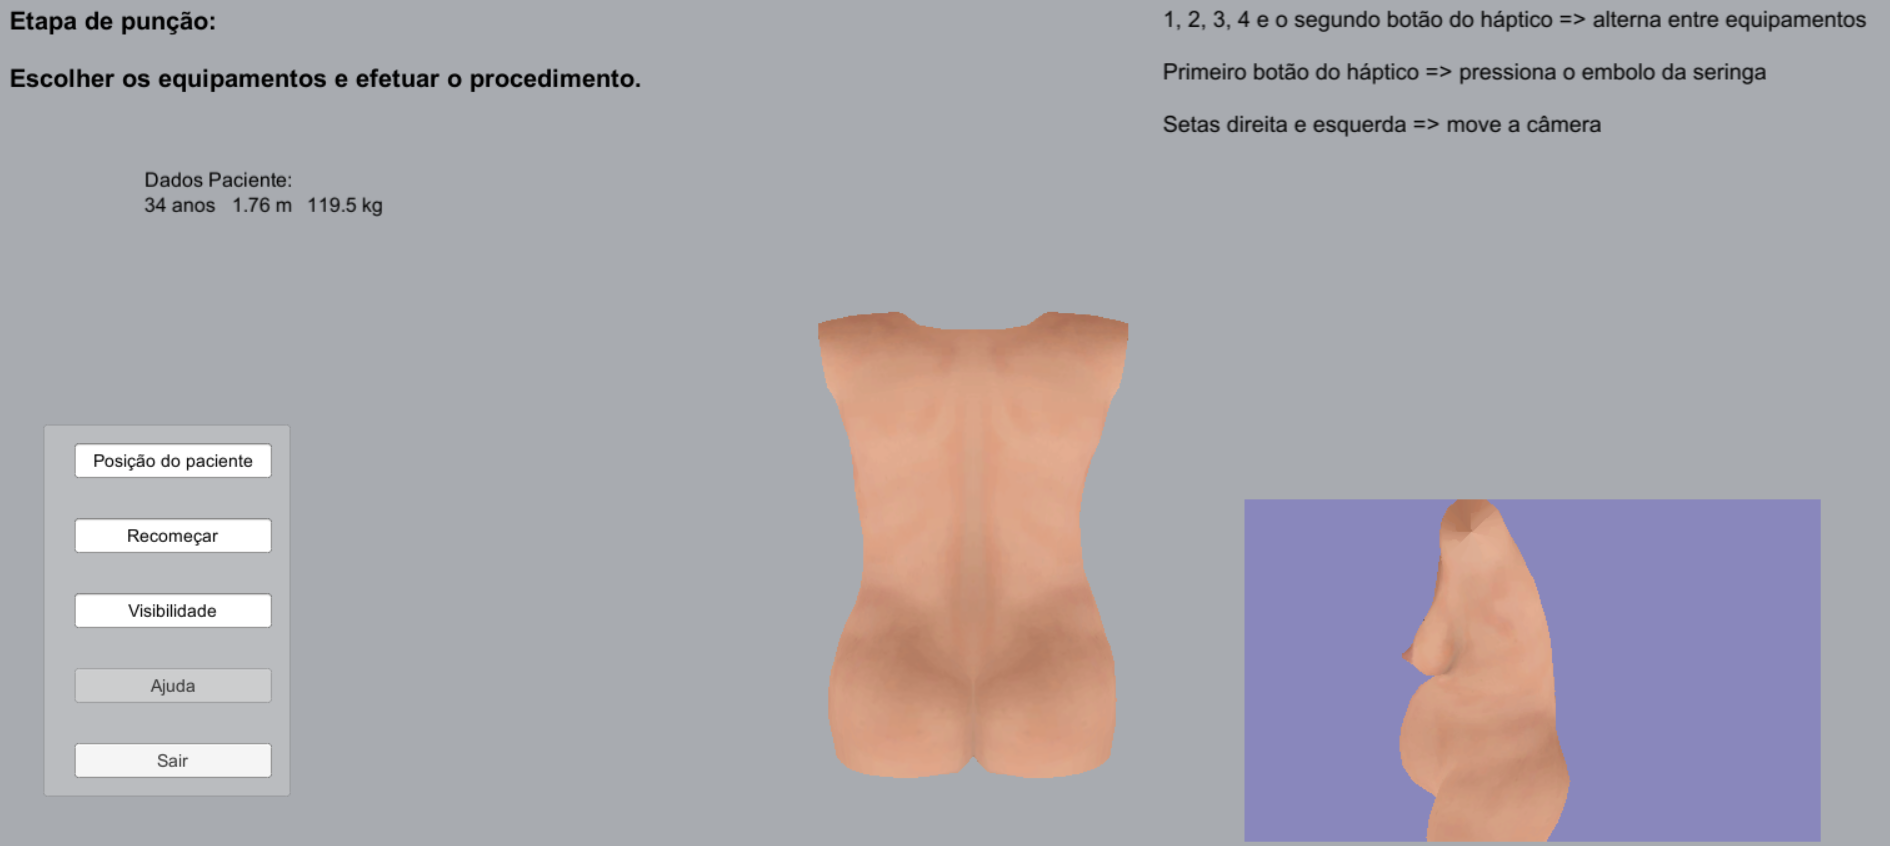
\includegraphics[width=0.9\linewidth]{capitulos/figuras/sistema posicao sentada.png} 
    \caption{Visão geral do sistema com tronco de paciente centralizada na tela na posição sentada. Do lado inferior direito a visão lateral desta mesma parte do corpo.}
    \label{fig:posicaoSentada}
\end{figure}

Uma outra opção de execução do procedimento incluída foi a possibilidade de mudança de posição da paciente que além da posição sentada (original e mais comum) agora também permite que o procedimento seja feito com ela deitada (estas são as duas posições em que ocorre o procedimento de raquianestesia \ref{sec:anestesiaRaquidiana}).

== MOSTRAR POSIÇÃO DEITADA ==

\subsection {Simulação de pacientes virtuais}

======
 MOSTRAR VARIAÇÕES DO CORPO PELAS TRANSFORMAÇÕES EXISTENTES
======  %inclui novo capítulo

\pagestyle{ruledheader}
\chapter{Testes de simulação} \label{cap:cap5}

Foram feitas avaliações das sensações proporcionadas pelo háptico como parte do projeto aprovado no comitê de ética do Hospital Universitário Antônio Pedro associado a faculdade de medicina da Universidade Federal Fluminense. Este projeto foi registrado na Plataforma Brasil do ministério da saúde sob o número 23637019.5.0000.5243 (texto no apêndice \ref{apend:comiteEtica}). A descrição destes experimentos e discussão dos resultados obtidos foram publicados em conferência da área \cite{Melo2021}.

Os experimentos foram apresentados a doze voluntários que fizeram uso do equipamento háptico, todos estes voluntários eram estudantes de ciência da computação com idades variando entre 18 e 44 anos sendo onze homens e uma mulher. Todos os voluntários concordaram com o termo de consentimento de participação nesta pesquisa (este está presente no apêndice \ref{apend:termoConsentimento}). Todos receberam uma breve explicação (cinco minutos) a respeito do procedimento de uso do equipamento háptico no experimento. Em seguida tiveram outros cinco minutos de tempo para usar um aplicativo de exemplo (para adquirir conhecimento sobre como interagir num ambiente com este tipo de dispositivo) visando nivelar o conhecimento.

Conforme comentado na seção anterior utilizamos o \textit{Haptic Plug-In For Unity3D} para programação das interações com o háptico utilizando o motor de jogo da \textit{Unity} \cite{UnityTechnologies2020} que é uma ferramenta muito utilizada para desenvolvimento de videogames e simulações com e sem \acrshort{RV} para diversas plataformas.
Este \textit{plugin} possibilita a interação do usuário com os objetos no ambiente virtual  de quatro modos distintos \cite{Poyade2014}. Para este experimento utilizamos o modo \textit{Puncture} (modo de punção) pelo requisito do experimento em simular uma agulha sendo inserida através de camadas representativas de tecidos.

O \textit{OpenHaptics driver} possui a definição de um conjunto de propriedades que representam como qualquer objeto 3D (camada, superfície, etc) tocável do ambiente virtual desenvolvido reage a cada interação com o dispositivo háptico. As propriedade mais relevantes no contexto do modo de punção são \textit{Stiffness}, \textit{Pop Through}, \textit{Static Friction}, e \textit{Dynamic Friction}. Todas elas têm como domínio um número real e aceitam valores entre zero e um. 

\textit{Stiffness} representa o nível de dureza do objeto: zero (0) representa um objeto mole e um (1) o objeto mais duro possível \cite{3DSystemsTouch2018}. Neste ponto é importante ressaltar que a quantidade de força máxima suportada depende das especificações do dispositivo háptico usado, dispositivos mais simples e de custo mais baixo comumente suportam intensidades de forças menores se comparadas a dispositivos mais complexos e com custos mais altos. \textit{Pop Through} controla o nível de força necessária para perfurar um objeto: zero indica que o objeto não pode ser perfurado e um que o máximo de força é necessário para perfurar o objeto \cite{3DSystemsTouch2018}. \textit{Punctured Static Friction} configura a dificuldade de se mover dentro de um objeto perfurado a partir de uma posição estática. O limite inferior (zero) representa um movimento sem atrito e o limite superior (um) representa a quantidade maior de atrito suportada pelo dispositivo \cite{3DSystemsTouch2018}. \textit{Punctured Dynamic Friction} controla a dificuldade de se mover dentro de um objeto depois que o movimento já foi iniciado \cite{3DSystemsTouch2018}. Da mesma forma que no caso estático o zero representa um movimento sem atrito e um o máximo de atrito suportado. Essas propriedades podem ser usadas para configurar o comportamento de cada camada de forma que o usuário tenha um experiência tátil de interação virtual que simule o procedimento real. As propriedades \textit{Stiffness} e \textit{Pop Through} precisam ser configuradas pra se determinar a força necessária por parte do usuário para perfurar cada objeto enquanto para determinar a força necessária para movimentação de uma agulha dentro de um objeto as propriedade a serem configuradas são \textit{Punctured Static Friction} e \textit{Punctured Dynamic Friction}.

Dois experimentos foram construídos para simular as diferentes sensações que os anestesistas experimentam enquanto executam punções lombares. Nestes experimentos os objetos 3D usados para simular as camadas do corpo foram simplificados e representados como hexaedros. Essa abordagem foi utilizada por que o objetivo destes experimentos era somente a avaliação das sensações de perfuração e deslocamento nas diferentes camadas proporcionadas pelo háptico e não algum tipo de avaliação estética. Deste modo foi removido o modelo 3D já desenvolvido para o simulador e foram utilizados modelos simplificados que não desviassem a atenção dos usuários do foco da avaliação. 
A Figura \ref{fig:visualExperimentos1e2} ilustra a forma que demonstramos visualmente os experimentos com elementos 3D com textura e sem transparência. Isto foi feito para que a resposta fosse somente de acordo com o retorno tátil obtido na mão do usuário ao usar o háptico sem dicas visuais a não ser o deslocamento da agulha. Incluímos um campo que demonstrava o deslocamento (profundidade) da agulha desde o início da perfuração pois algumas perguntas que formulamos nos experimentos dependiam do conhecimento destas distâncias entre o ponto de perfuração e cada uma das sensações. O usuário movimenta o elemento 3D que representa a agulha através do dispositivo háptico. Incluímos uma visão lateral a direita para que fosse possível observar a agulha e os objetos sendo perfurados de perfil. Desta forma foi possível observar facilmente quando a agulha estava totalmente inserida no objeto em cada experimento.
As imagens dos detalhes dos objetos 3D dos dois experimentos podem ser visualizados na Figura \ref{fig:objectsExperiments}. As setas de diferentes tamanhos no eixo Z ilustram as diferenças nos objetos 3D de cada experimento. A primeira camada (mais externa) é um cubo, e as demais camadas tem profundidades menores mas todas tem a mesma largura (eixo X) e altura (eixo Y), como pode ser visto na Figura \ref{fig:objectsExperiments}.

\begin{figure}[ht!]
    \centering
    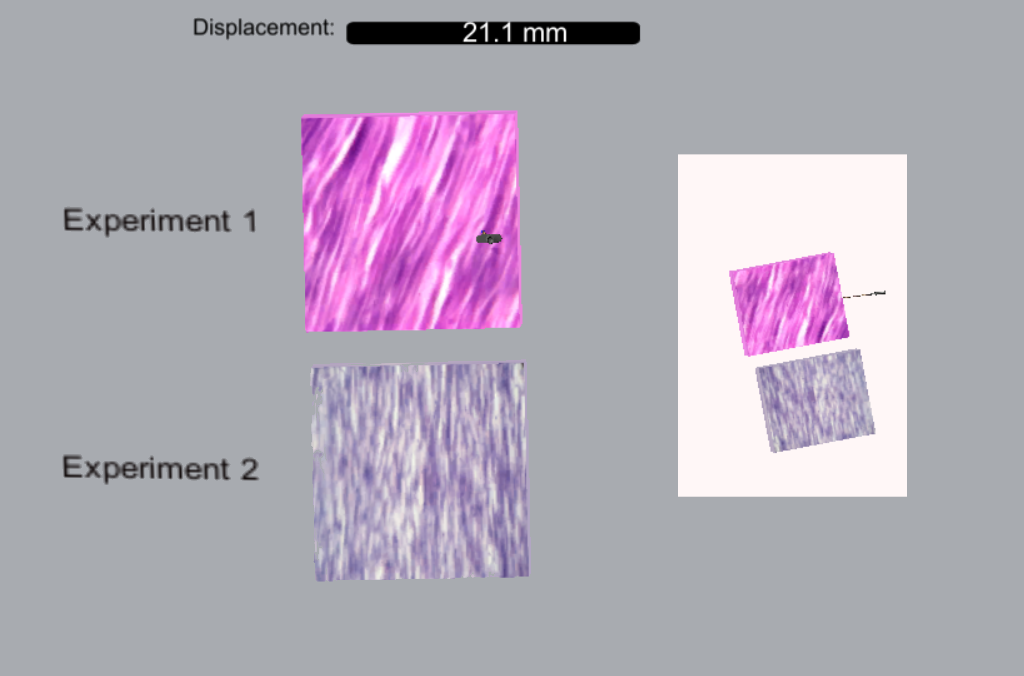
\includegraphics[width=0.8\linewidth]{capitulos/figuras/visual-experimentos.png} 
    \caption{Aparência visual dos experimentos 1 e 2. Na esquerda a vista de frente e na direita com fundo branco a vista lateral. As diferenças nas dimensões ocorrem somente na profundidade das camadas internas.}
    \label{fig:visualExperimentos1e2}
\end{figure}

\begin{figure}[ht!]
    \centering
        \begin{tabular}{cc}
        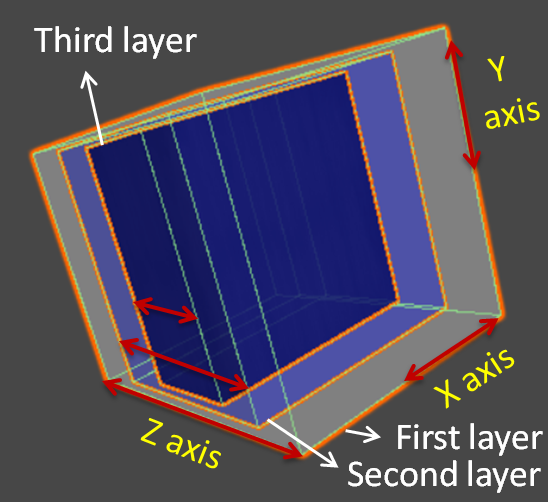
\includegraphics[width=0.3\linewidth]{capitulos/figuras/First.Experiment - axis.PNG} & 
        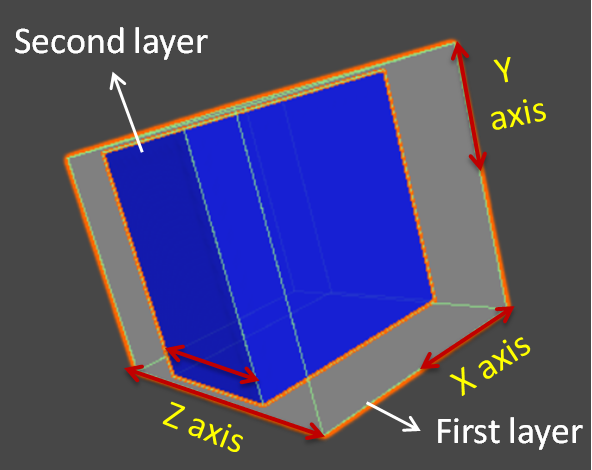
\includegraphics[width=0.35\linewidth]{capitulos/figuras/Second.Experiment - axis.PNG} 
        \\
        (a) & (b)
        \end{tabular}
    \caption{Os objetos 3D representam as camadas de cada experimento: (a) Primeiro experimento (b) Segundo experimento.}
    \label{fig:objectsExperiments}
\end{figure}

O tamanho da agulha é 65 milímetros (mm). Para os dois experimentos foi incluída uma deformação na interface de cada camada com o aumento da força antes da perfuração. Essa deformação é uma função da força necessária para perfurar cada camada. Foi usado um valor máximo de deformação de cinquenta vezes o valor da propriedade \textit{Pop through} em cada camada. O deslocamento desta deformação máxima é medido em milímetros. Logo após ser perfurado o tecido reassume a posição original (sem deformação). 

A Tabela \ref{tab:propHapticoPrimeiroExperimento} descreve os valores configurados nas propriedades de cada camada do primeiro experimento. A deformação máxima para a primeira camada é de 2,5 mm, que corresponde a cinquenta vezes 0,05 (\textit{Pop Through} da primeira camada). A Figura \ref{fig:forcaDeslocamentoExperimento1} apresenta um gráfico da força aplicada (eixo vertical) com o deslocamento da agulha representado no eixo horizontal para o experimento 1. As setas nesta imagem indicam a extensão da deformação de cada camada, começando na esquerda quando a agulha começa a tocar a camada e terminando na direita quando a camada é perfurada. O deslocamento da agulha observado na área sob as setas representa menores variações por conta da necessidade do aumento de força que vai deslocando lentamente a agulha enquanto deforma a camada até o momento em que a camada é perfurada. O espaço entre as setas da Figura \ref{fig:forcaDeslocamentoExperimento1} representa quando a agulha está em movimento dentro das camadas. 
As diferenças mais significativas no eixo de deslocamento podem ser observados a direita das setas, marcados com retângulos, que representa o aumento da velocidade de deslocamento da agulha imediatamente após a perfuração da camada.

\begin{table}[!ht]
\begin{center}
\caption{Configurações das propriedade do \textit{plugin} do háptico usadas no primeiro experimento.}
\label{tab:propHapticoPrimeiroExperimento}
\begin{tabular}{|l|lll|}
\hline
\multicolumn{1}{|c|}{\multirow{2}{*}{Propriedade}} & \multicolumn{3}{c|}{Camada}  \\ \cline{2-4} 
\multicolumn{1}{|c|}{} & \multicolumn{1}{c|}{1} & \multicolumn{1}{c|}
{
\begin{tabular}[c]{@{}c@{}}2\end{tabular}} & \multicolumn{1}{c|}{\begin{tabular}[c]{@{}c@{}}3\end{tabular}}  \\ 
\hline\hline
\textit{Stiffness} & \multicolumn{1}{l|}{0,75} & \multicolumn{1}{l|}{0,75} & \multicolumn{1}{l|}{0,75} \\ 
\textit{Pop Through} & \multicolumn{1}{l|}{0,05} & \multicolumn{1}{l|}{0,15} & \multicolumn{1}{l|}{0,10}  \\ 
\textit{Punctured Static Friction} & \multicolumn{1}{l|}{0,20} & \multicolumn{1}{l|}{0,30} & \multicolumn{1}{l|}{0,30}  \\ 
\textit{Punctured Dynamic Friction} & \multicolumn{1}{l|}{0,30} & \multicolumn{1}{l|}{0,30} & \multicolumn{1}{l|}{0,10}  \\ 
\hline
\end{tabular}
\end{center}
\end{table}

O segundo experimento tem duas camadas e sua configuração é descrita na Tabela \ref{tab:propHapticoSegundoExperimento}. A curva de força versus deslocamento da agulha desse experimento está ilustrada na Figura \ref{fig:forcaDeslocamentoExperimento2} e aqui se aplicam as mesmas considerações feitas em relação as marcações de setas e retângulos discutidas em relação a Figura \ref{fig:forcaDeslocamentoExperimento1}.

O ponto de referência considerado para a interface da primeira camada em cada experimento foi 0 mm. Esta referência serve para medir o deslocamento da agulha a partir do toque na primeira camada até atingir todas as demais camadas. Esta medida é feita na direção ortogonal à superfície da camada tocada pelo usuário com a agulha virtual. A segunda camada do primeiro experimento está posicionada a 25 mm a partir desta referência e a terceira camada está a 50 mm. A segunda camada do segundo experimento inicia a 35mm do ponto de referência.

\begin{figure}[ht!]
    \centering
    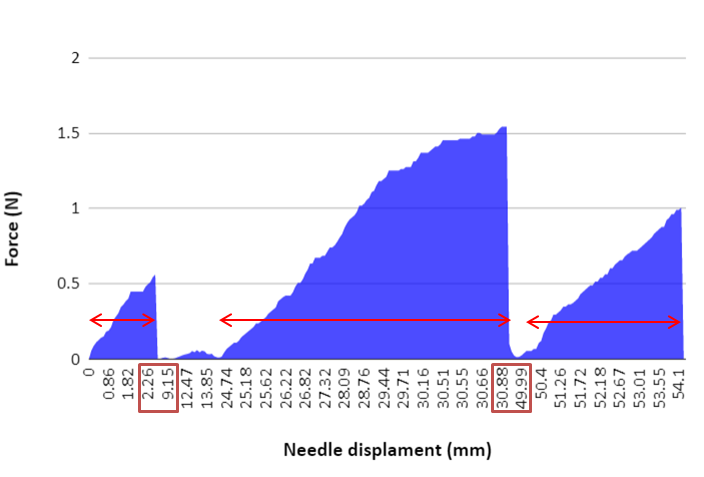
\includegraphics[width=0.8\linewidth]{capitulos/figuras/Experiment 1 - Force x Needle displacement - marked.PNG} 
    \caption{Relação entre força e o deslocamento da agulha média considerando dez simulações no experimento 1.}
    \label{fig:forcaDeslocamentoExperimento1}
\end{figure}

\begin{table}[!ht]
\begin{center}
\caption{Configurações das propriedade do \textit{plugin} do háptico usadas no segundo experimento.}
\label{tab:propHapticoSegundoExperimento}
\begin{tabular}{|l|ll|}
\hline
\multicolumn{1}{|c|}{\multirow{2}{*}{Propriedade}} & \multicolumn{2}{c|}{Camada}  \\ \cline{2-3} 
\multicolumn{1}{|c|}{} & \multicolumn{1}{c|}{1} & \multicolumn{1}{c|}{\begin{tabular}[c]{@{}c@{}}2\end{tabular}}  \\  
\hline\hline
\textit{Stiffness} & \multicolumn{1}{l|}{0,75} & \multicolumn{1}{l|}{0,20}  \\ 
\textit{Pop Through} & \multicolumn{1}{l|}{0,05} & \multicolumn{1}{l|}{0,15}  \\ 
\textit{Punctured Static Friction} & \multicolumn{1}{l|}{0,90} & \multicolumn{1}{l|}{0,10}  \\ 
\textit{Punctured Dynamic Friction} & \multicolumn{1}{l|}{0,20} & \multicolumn{1}{l|}{0,10}   \\ 
\hline
\end{tabular}
\end{center}
\end{table}

\begin{figure}[ht!]
    \centering
    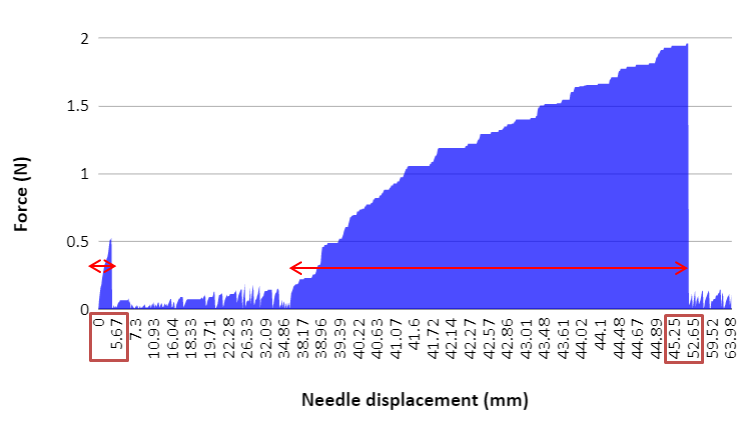
\includegraphics[width=0.8\linewidth]{capitulos/figuras/Experiment 2 - Force x Needle displacement - marked.PNG} 
    \caption{Relação entre força e o deslocamento da agulha da média de dez simulações no experimento 2.}
    \label{fig:forcaDeslocamentoExperimento2}
\end{figure}

A quantidade de camadas de cada experimento proposto aqui difere do número original de camadas do procedimento descrito na seção~\ref{sec:anestesiaRaquidiana}. Isto por que a ideia aqui não foi representar todo o corpo ou procedimento. A ideia foi reproduzir, nos experimentos, as sensações mais importantes e críticas envolvidas neste procedimento. As outras interfaces entre as camadas são simples reproduções de partes das que foram incluídas nestes experimentos.

\section{Questionário}
\label{sec:questionario}

Após o tempo de testes com a ferramenta de nivelamento no uso do háptico e antes do início do tempo do experimento os questionários com as perguntas de cada experimento foram apresentados para os usuários. Isto foi feito de forma que durante o experimentos cada um pudesse coletar as informações necessárias para responder cada pergunta. Apresentamos a seguir as perguntas dos questionários que foram apresentadas para os voluntários.

Questão 1) Experimentos número 1 e 2: Quantas camadas você pode sentir desde o momento de perfurar o objeto até chegar ao deslocamento máximo de 65mm? 
Observação: Cada camada é identificada por uma restrição a perfuração.

Questão 2) Experimento número 1: Ordene as camadas de forma decrescente em relação a resistência a perfuração.    
Exemplo de resposta: 1, 2 (considerando que existam duas camadas e a primeira é mais resistente que a segunda).

Questão 3) Experimento número 1: Em qual posição cada camada começa, ou seja, qual o ponto do deslocamento da agulha onde você identificou resistência para perfuração? 
Exemplo de resposta: Camada 1 = 0mm, Camada 2 = 10mm e Camada 3 = 30mm (considerando que tenham sido identificadas 3 camadas com resistências nestes 3 pontos de deslocamento).

Questão 4) Experimento número 2: Em qual intervalo (início e fim) de deslocamento foi observado a maior resistência ao movimento de perfuração? 
Exemplo de resposta: Entre 10mm e 20mm.

Questão 5) Experimento número 2: Em qual intervalo (início e fim) de deslocamento foi observado uma necessidade de aplicação de uma força constante para o deslocamento? 
Exemplo: Entre 10mm e 20mm.

Todas as perguntas envolvem aspectos de identificação tátil vitais na realização de uma raquianestesia. Os exemplos de resposta foram ilustrados com o intuito de facilitar a posterior análise das respostas procurando evitar excessos de descrições desnecessárias. A identificação do comportamento elástico é avaliado nas questões 1, 3 e 5 enquanto a questão 4 trata da identificação do comportamento plástico. A questão que envolve a identificação da posição inicial (3) e as que pedem a identificação de intervalos de comportamentos (4 e 5) avaliam a sensação de deformação de cada camada. Todas as camadas iniciam na sua posição de origem e possuem uma deformação imediatamente antes da perfuração que deslocam esta posição. Para fins de avaliação, consideramos corretas as respostas entre o ponto inicial e o ponto final de deformação nas identificações de interface de cada camada.  

\section{Respostas}
\label{sec:respostas}

Nesta seção apresentamos uma compilação das respostas dos participantes às perguntas de cada experimento. Para o primeiro
experimento, as respostas foram as seguintes:

Questão 1) Onze voluntários (aproximadamente 92\%) responderam corretamente.

Questão 2) Sete voluntários (58\%) responderam corretamente para todas as camadas. Onze voluntários (92\%) acertaram a camada menos resistente e nove (75\%) acertaram a mais resistente.

Questão 3) Nove voluntários (75\%) responderam corretamente para todas as camadas. Todos acertaram a segunda camada e onze voluntários (92\%) acertaram a primeira camada.

Após responder o primeiro questionário as mesmas pessoas executaram o segundo experimento e responderam o questionário deste conforme descrito a seguir:

Questão 1) Todos os voluntários (100\%) responderam corretamente.

Questão 4) Nove voluntários (75\%) responderam corretamente.

Questão 5) Cinco voluntários (42\%) responderam corretamente. Nove (75\%) acertaram o início.

\section{Avaliação dos resultados}
\label{sec:avaliacao}

Nesta seção detalhamos cada um dos comportamentos mais importantes do procedimento coberto nestes experimentos que foram criados para avaliar a percepção do usuário sobre o comportamento das
camadas virtuais sendo perfuradas por uma agulha.

\subsection{Resistência à punção}

Considerando os sentimentos ou sensações resistência à punção (o assunto da questão dois), apenas 58\% dos respondentes ordenaram corretamente todas as camadas de acordo com suas resistências. Este resultado indica a necessidade de se aumentar a diferença na força necessária para perfurar cada camada para permitir uma identificação mais facilitada de todas estas características. Na mesma pergunta, um número maior de voluntários identificaram a camada mais resistente ou a menos resistente à perfuração. Essa identificação é essencial para indicar quando a agulha penetra no ligamento amarelo (tecido mais resistente) ou a dura-máter (tecido menos resistente). Como estas duas camadas estão posicionadas no corpo humano uma após a outra (considerando o ângulo de perfuração correto), a correta identificação de uma é, por si só, um passo essencial na simulação correta do procedimento de raquianestesia.

\subsection{Comportamento elástico}

Quanto à identificação do comportamento elástico (questões 1, 3 e 5), apenas a questão cinco recebeu pontuação inferior a 75\%. No entanto, mesmo nesta questão, apenas três voluntários apontaram erroneamente o ponto de partida do intervalo com maior restrição ao movimento da agulha. Assim, quase todos os participantes puderam apontar onde esta camada começa. No entanto, o mesmo resultado não foi alcançado na identificação do seu fim, com mais da metade (58\%) perdendo o ponto final. Analisando as respostas e o modelo, a causa mais provável disso indica que o curva utilizada foi muito alta, pois houve uma queda significativa na pressão e grande deslocamento da agulha quando o usuário deixou este camada. Assim, se identificar o final da camada é essencial para o problema, é necessário reduzir a queda de pressão no modelo para melhor simular esse comportamento.

Tivemos ótimas respostas na detecção do número de camadas (questão um) em todos experimentos. Identificar as camadas penetradas é uma das partes mais críticas do procedimento de raquianestesia. Isto indica tanto a determinação correta da sensação de \textit{popping} da interface entre as camadas e reconhecimento do comportamento elástico que ocorre imediatamente antes de perfurar cada camada.

Quanto à identificação do ponto de início de cada camada, o assunto da questão três, também é importante destacar o número de casos corretamente identificados (75\%). Esta resposta reforça a necessidade de utilização de valores de profundidade desde a pele até o espaço subaracnóide próximo da realidade para treinar melhor os anestesistas. Cada ponto de partida da camada está relacionado com o início do comportamento elástico e é necessário aumentar a força para prosseguir com o avanço da agulha em cada interface entre camadas.

\subsection{Comportamento plástico}

A questão quatro, com 75\% de sucesso na identificação, aborda um outro comportamento de grande importância na raquianestesia. A identificação de estar dentro da camada que apresenta a maior
resistência, ou seja, sentir uma pressão constante contra o movimento através da camada (comportamento plástico), está relacionado ao ligamento amarelo, que ocorre imediatamente antes de se atingir o espaço peridural. As respostas a esta pergunta
confirmam que esse comportamento pode ser simulado adequadamente.  %inclui novo capítulo

\pagestyle{ruledheader}
\chapter{Considerações Finais} \label{cap:cap6}

\section{Conclusão}
\label{sec:conclusão}

A contribuição principal deste trabalho está na reprodução virtual das principais sensações hápticas necessárias para simular a anestesia raquidiana. Outra contribuição que é uma etapa fundamental para tornar a simulação mais real e adaptável a vários cenários de testes foi a construção de um modelo 3D do tronco de uma gestante de forma facilmente modificável via programação. A variabilidade de pacientes que pode ser configurada usando o modelo proposto é bastante vasta. Foi também descrito o passo a passo das formas de uso da \textit{engine} da \textit{Unity} e do \textit{plugin} para importação do modelo e interação deste com o háptico na simulação. 

Foram feitos experimentos para avaliar a eficiência da simulação a partir do uso das ferramentas hápticas disponíveis com configurações sugeridas com o intuito de representar as principais sensações experienciadas por anestesistas durante o procedimento da raquianestesia. Através de questionários objetivos procuramos reduzir a subjetividade das respostas nas análises destas sensações.

Em relação a área médica no treinamento de anestesia raquidiana a ideia principal é o uso de alguns níveis de treinamento com o simulador visando evitar que pacientes sejam atendidos por pessoas sem antes participar de um treinamento prático.

\section{Trabalhos Futuros}
\label{sec:trabFuturo}

Outras partes do corpo, inclusão de \textit{feedback} de dor do paciente para movimentos bruscos    %inclui novo capítulo

\pagestyle{ruledheader}
\chapter{Considerações Finais} \label{cap:cap7}

O uso de um simulador no treinamento ajuda a atenuar riscos de falhas da raquianestesia relacionados a habilidades médicas não adquiridas corretamente assim como reduzir custos de laboratório e peças pra reposição de modelos físicos. Foram simulados aqui os comportamentos necessários para representar a agulha espinhal penetrando através dos vários ligamentos e tecidos do corpo. Um simulador de raquianestesia de alta fidelidade requer recursos como haver uma região das costas com a sensação de vértebras da coluna que possam ser localizadas por palpação, a capacidade de acomodar várias posições do paciente, inclinações ajustáveis de inserção da agulha e alguns outros aspectos principais. Todos estes itens citados em específico são contemplados no simulador criado aqui, que inclui um modelo 3D criado e utilizado juntamente com os parâmetros e configurações descritas nesta tese. 

Nos experimentos, o objetivo foi de simular corretamente as sensações táteis essenciais da punção da agulha durante o procedimento de raquianestesia. A identificação das transições entre os tecidos foi um dos comportamentos levado em consideração, por ser imprescindível na representação do caso real e, portanto, no treinamento deste procedimento médico.
A variação da resistência ao movimento da agulha em cada tecido foi outro comportamento considerado. O resultado dos experimentos mostrou que as opções de configurações presentes nas ferramentas táteis programáveis são capazes de representar esses comportamentos.

Não foram feitas avaliações do uso do ambiente de simulação desenvolvido nesta tese em relação a ergonomia, porém, foram feitas adaptações da montagem dos equipamentos nos testes com especialistas. Estas variações na montagem foram feitas por sugestão dos próprios anestesistas para que eles executassem o procedimento no ambiente de treinamento em posição similar aquela que estão acostumados a conduzir o procedimento real.

\section{Conclusão}
\label{sec:conclusão}

Nesta tese de doutorado foi criado ambiente virtual para treinamento do procedimento de raquianestesia em gestantes desde a palpação até a administração do anestésico. A solução proposta para a Questão~\ref{prob:simuladorCasoReal} apresenta um ambiente com avaliação do desempenho dos usuários de acordo com suas sequências de execução dos procedimentos, bem como apresenta uma forma totalmente virtual para representação da palpação da coluna através do uso de um dispositivo háptico.

Dentre as contribuições deste trabalho está a reprodução virtual das principais sensações hápticas necessárias para simular a anestesia raquidiana. Foram feitos experimentos para avaliar a eficiência da simulação a partir do uso das ferramentas hápticas disponíveis. O sistema foi avaliado quanto a sua usabilidade de forma quantitativa através do método \textit{\acrshort{SUS}} \cite{Brooke2013} tendo como resposta a classificação de usabilidade boa. Especialistas fizeram uso do ambiente de simulação e responderam questionários de avaliação. Estes informaram considerar como útil este tipo de treinamento. Os anestesistas recomendaram algumas melhorias visando aproximar o simulador ainda mais do procedimento real e, desta forma, poder ser de fato utilizado como ferramenta de treinamento de anestesia raquidiana. Na comparação com o simulador de Färber et al. \cite{Farber2008} as avaliações do simulador desta tese obtiveram notas inferiores, porém, como comentado na Seção~\ref{sec:avaliacaoEspecialistas}, não foi possível reproduzir o mesmo cenário e nem o mesmo equipamento (dispositivo háptico) nos testes. É importante ressaltar que, apesar das notas menores, o simulador desta tese tem duas das características principais de simuladores de punção mais completos que o simulador de Färber et al. \cite{Farber2008} não possui. O simulador apresentado nesta tese possibilita a palpação da coluna para escolha do ponto de inserção da agulha. Esta característica só existe em outros dois dos simuladores computacionais estudados nesta tese (nenhum destes simula a anestesia raquidiana). A outra característica é que com o modelo 3D adaptável desenvolvido nesta tese é possível a simulação de múltiplas pacientes. O simulador de Färber et al. \cite{Farber2008} possui somente três (3) representações de pacientes.

Outra contribuição que é uma etapa fundamental para tornar a simulação mais real e adaptável a vários cenários de testes foi a construção de um modelo 3D do tronco de uma gestante de forma facilmente modificável via programação. A variabilidade de pacientes que pode ser configurada usando o modelo proposto é bastante vasta. Para uma maior reprodução do caso real no que diz respeito à espessura das principais camadas, o modelo foi alimentado por um equação genérica desenvolvida neste trabalho. Foi também descrito o passo a passo das formas de uso da \textit{engine} da \textit{Unity} e do \textit{plugin} para importação do modelo e interação deste com o háptico na simulação. 

Em relação à evolução dos simuladores atualmente disponíveis para raquianestesia a contribuição desta tese envolveu a simulação virtual da palpação. Outra contribuição neste sentido foi a construção de um ambiente para treinamento de raquianestesia (e não somente um simulador). Este ambiente apresenta \textit{feedbacks} durante e após cada procedimento. Propomos aqui uma avaliação do desempenho de cada procedimento por meio de notas bem como a avaliação combinada de todos os procedimentos feitos pelo usuário. 

\section{Limitações}

Descrevemos nesta Seção as principais limitações deste trabalho. A primeira se refere ao dispositivo háptico que tivemos a oportunidade de adquirir e utilizar no desenvolvimento deste trabalho. O dispositivo é um modelo mediano, não exatamente com todos os graus de liberdade e a capacidade de reprodução das forças necessárias a uma completa representação do que seria uma movimentação da agulha. O dispositivo utilizado nesta tese não permite a simulação de forma completa de todas as restrições de movimento para representação da movimentação da agulha após a mesma ser inserida no paciente. Devido ao alto custo, não foi possível viabilizar o uso de um modelo mais avançado que possui mais graus de liberdade e possibilidade de representação de força, rotações e torções mais adequadas. Isto fez com que parte da realidade do procedimento ficasse comprometida. Em relação aos graus de liberdade de movimento, esta limitação impactou o realismo, pois quando uma agulha é inserida na pele (no procedimento real) existe uma força que impede o movimento de rotação lateral da agulha, que não é possível ser representado pelo equipamento utilizado nesta tese. Com relação à força máxima suportada pelo aparelho, o impacto no realismo aconteceu quando voluntários, ao usarem o simulador, sentiram uma resistência ao avanço da agulha ou ao toque na pele. Neste caso, a reação de alguns voluntários foi a de aumentar a força aplicada, ultrapassando o limite suportado pelo háptico. Quando esse tipo de situação ocorre, o equipamento é projetado para liberar o avanço de forma a evitar danos ao seus mecanismos (procedimento de segurança do dispositivo), o que ocasiona uma perda da imersão da sensação háptica.

Existem outras limitações relacionadas à forma como foram realizados as pesquisas que obtiveram as respostas aos questionários na última fase dos testes realizados no Hospital Universitário Antônio Pedro (HUAP). Uma delas foi a restrição de tempo dos especialistas para realizarem os testes. Outra foi a ausência de um grande número de voluntários residentes, ou seja, estudantes ainda em treinamento em anestesia, o que inviabilizou uma reprodução de experimento mais justa no que diz respeito a comparação que foi efetuada com o similador desenvolvido na pesquisa de Färber et al. \cite{Farber2008}. Para viabilizar o acesso ao maior número de especialistas para avaliação do ambiente de simulação foi necessário efetuar a montagem do háptico e do laptop na secretaria do centro cirúrgico do HUAP, aproveitando o tempo dos especialistas, no intervalo entre cirurgias. O cenário ideal seria uma montagem num local reservado sem assistência, visão, ou influência de colegas no momento da simulação, como acabou acontecendo no teste de parte dos voluntários. 

\section{Trabalhos Futuros}
\label{sec:trabFuturo}

Uma próxima etapa, idealmente, envolveria profissionais instrutores de procedimentos de raquianestesia de forma a validar a possibilidade do uso do simulador no treinamento. Isso, após um passo inicial de avaliação para inclusão de novas funcionalidades ou remodelagem de funcionalidades existentes, adequando este simulador às necessidades de treinamento. Alguns exemplos de adequações a serem feitas, mesmo sem esse contato com especialistas, poderiam envolver, por exemplo, a representação virtual do escorrimento do líquor quando a agulha fica por alguns segundos no espaço subaracnóideo e a modelagem de toda a paciente, incluindo as demais partes do corpo para um ambiente ainda mais completo em termos de imersão. Ainda visando uma representação mais fiel da realidade, a inclusão de \textit{feedback} de dor da paciente para possíveis movimentos bruscos de objetos perfurantes no seu corpo pode ser incluída. Uma opção é usar um sintetizador de voz para este fim. A inclusão de óculos 3D (uma das principais questões trazidas na avaliação pelos especialistas) traria benefícios em relação à imersão ainda que tendo o custo deste equipamento. O uso deste tipo de equipamento é uma realidade possível em hospitais e universidades com melhor estrutura para treinamento.
Em relação à generalização e aproveitamento do trabalho feito na construção do modelo 3D é possível fazer o uso deste modelo para outros tipos de procedimentos que forem efetuados na mesma área do corpo (dorso). Este foi mais um ponto levantado por diversos especialistas, falando sobre outros tipos de procedimentos onde este tipo de simulador também faria sentido.

A aplicação de técnicas para reconhecimento de engajamento por parte do usuário \cite{Mitsis2022} é uma opção que poderia ser usada para alterar rumos do treinamento.
Outro caminho de trabalho futuro está no uso de realidade aumentada no lugar do dispositivo háptico usando a identificação da mão e incluindo esta no ambiente virtual. Nesta abordagem, no momento da punção, seria incluída a agulha ou seringa na mão da pessoa usando o simulador. Para tornar possível esta prática é preciso o estudo de formas de ``enganar'' o cérebro humano para que este perceba a resistência ao avançar da mão no ambiente virtual mesmo sem que algo físico impeça este movimento (como acontece no caso real e com a simulação com o háptico). Uma vez encontrada esta solução, a abordagem ganharia em flexibilidade e teria o custo reduzido por conta da ausência da necessidade de existência do dispositivo háptico. Um rumo que envolve tecnologias recentes para esta área seria o de modelar uma nova arquitetura do ambiente de treinamento com a integração de conceitos de internet das coisas \cite{Ahmad2022}.  %inclui novo capítulo

%\pagestyle{ruledheader} %inclui novo capítulo
%\chapter{Fundamentação Teórica} \label{cap:cap2}

Este Capítulo relaciona os conceitos e as tecnologias envolvidas no desenvolvimento do ambiente de treinamento proposto. 

\section{Anestesias Regionais}

Anestesias são atualmente usadas em diversos procedimentos cirúrgicos na medicina tradicional com o intuito de bloquear temporariamente a capacidade do cérebro de reconhecer um estímulo doloroso. Esta prática visa permitir a execução de procedimentos invasivos por parte do médico enquanto mantém o conforto e a tranquilidade do paciente. A anestesia regional é um procedimento usado em cirurgias onde o paciente pode permanecer acordado. Este tipo de anestesia bloqueia a dor em apenas uma determinada região do corpo, como um braço, uma perna ou toda região inferior do corpo, abaixo do abdômen \cite{Pinheiro2018}.

Os dois tipos de anestesias regionais mais usados são: anestesia raquidiana (ou raquianestesia, raqui), e anestesia peridural ou epidural. Estes dois tipos de anestesias também são conhecidas como anestesias de neuroeixo ou ainda bloqueio de neuroeixo \cite{Pinheiro2018}. Ambas podem ser aplicadas com pacientes sentados e inclinados para frente ou deitados de lado \cite{Anesclin2019}. 

\begin{figure}[ht!]
    \centering
    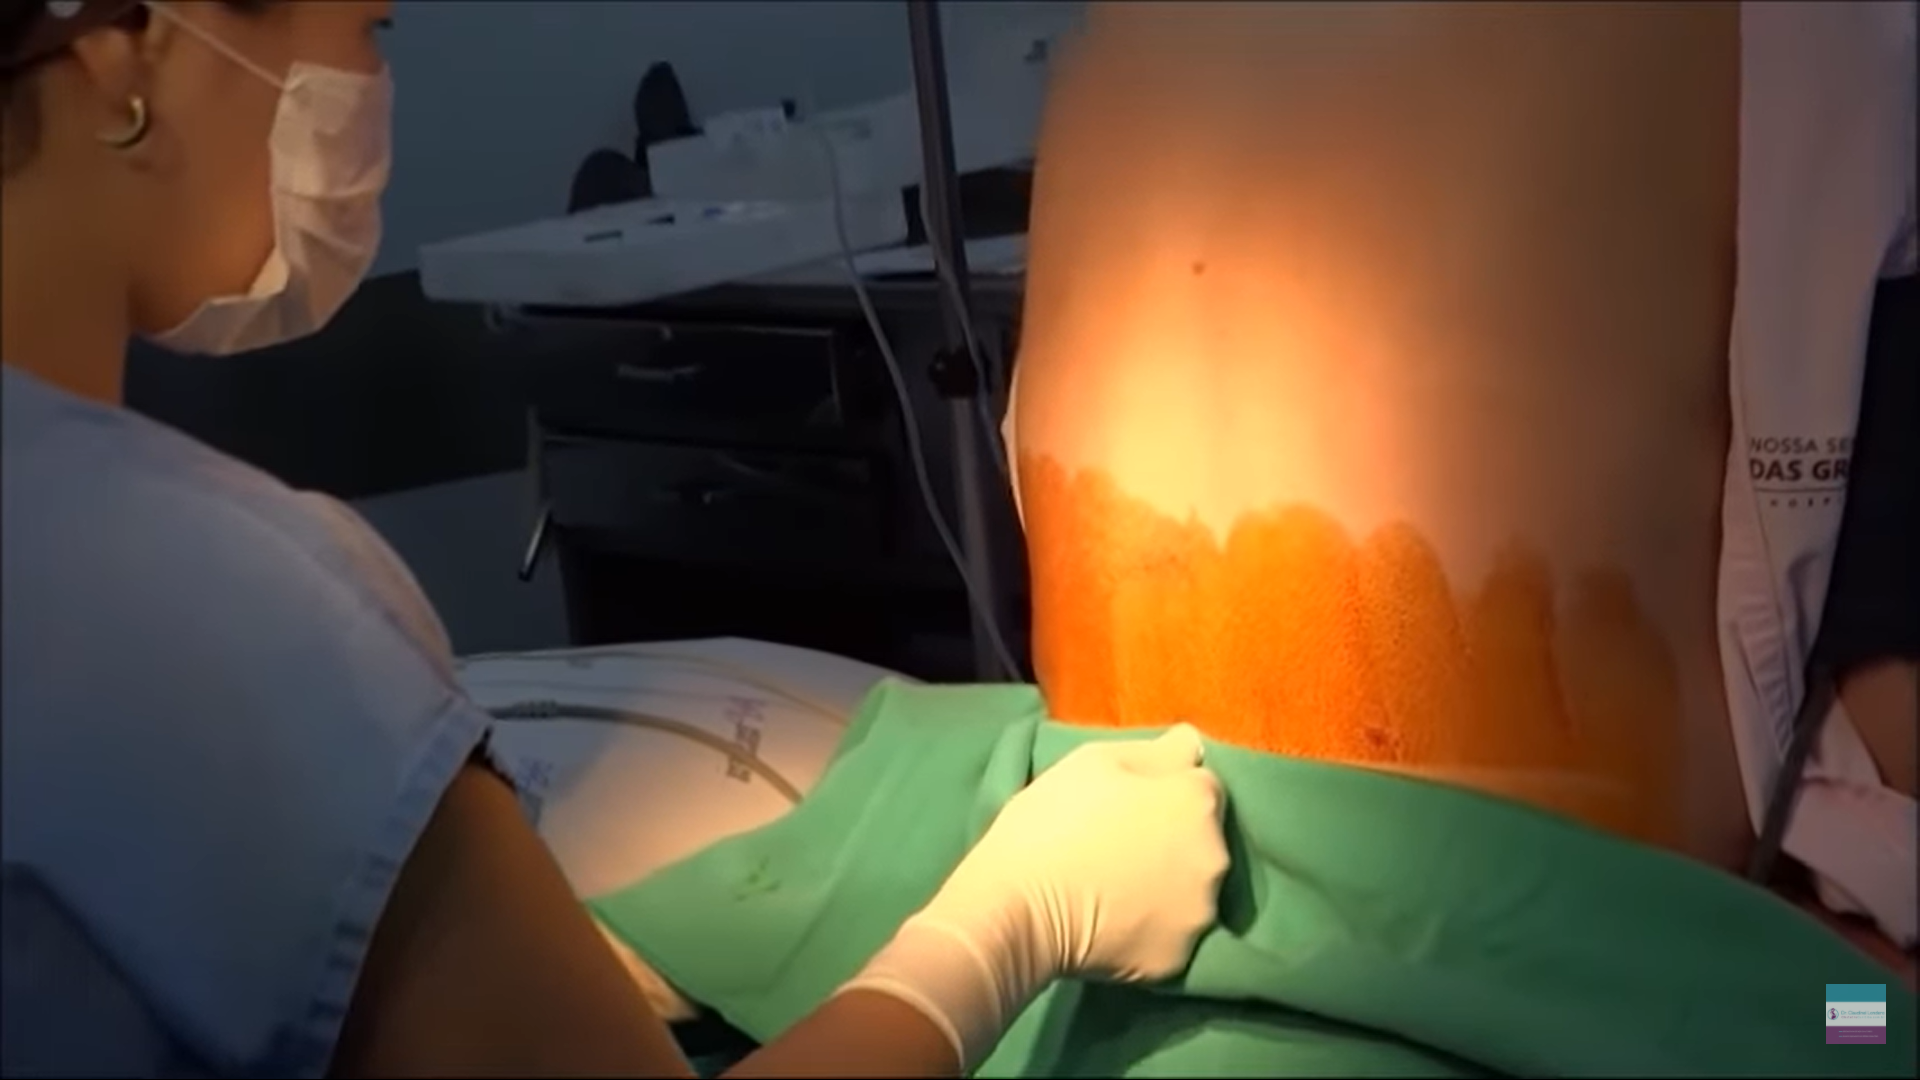
\includegraphics[width=0.6\linewidth]{capitulos/figuras/0.marcacaoPonto.png}
    \caption{Palpação para determinação do ponto de inserção da agulha \cite{Londero2018}.}
    \label{fig:marcacaoPonto}
\end{figure}

\begin{figure}[ht!]
    \centering
    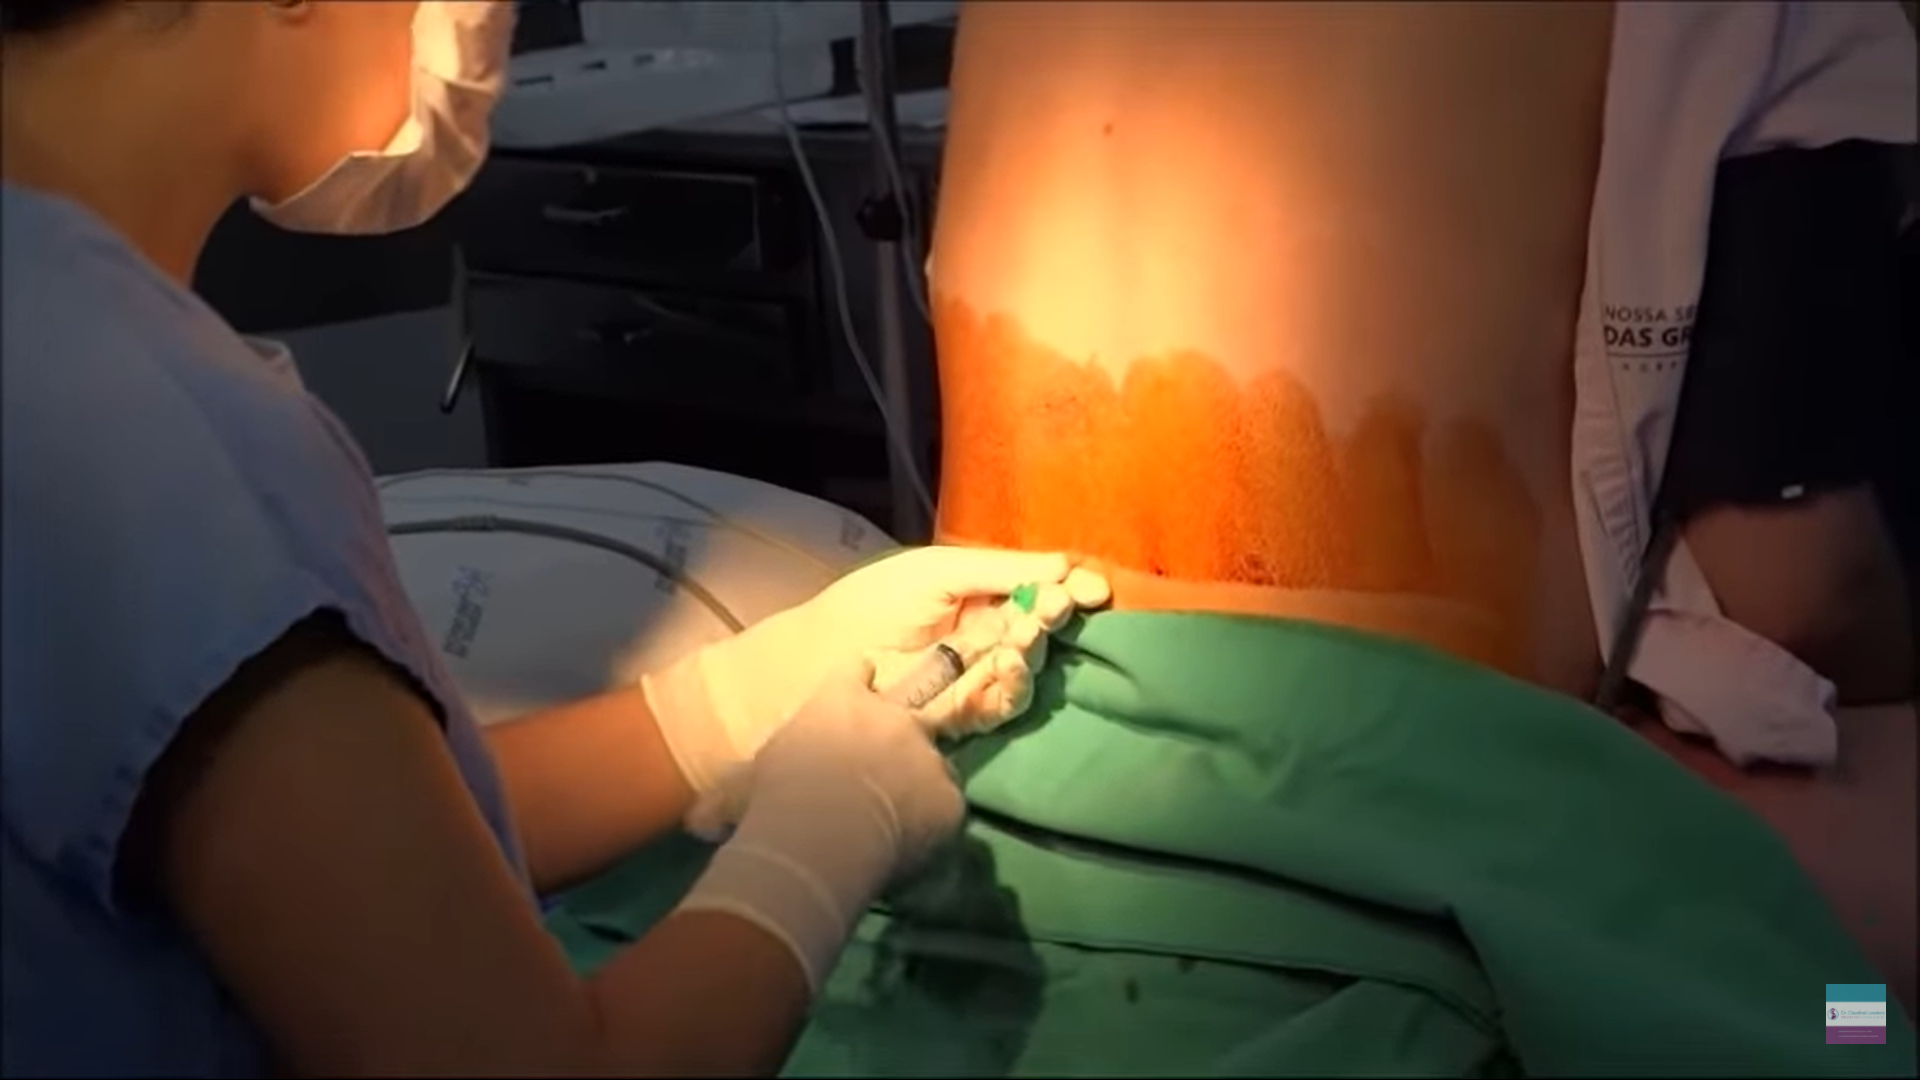
\includegraphics[width=0.6\linewidth]{capitulos/figuras/1.AnestesiaLocal.png}
    \caption{Aplicação da anestesia local \cite{Londero2018}.}
    \label{fig:anestesiaLocal}
\end{figure}

\begin{figure}[ht!]
    \centering
    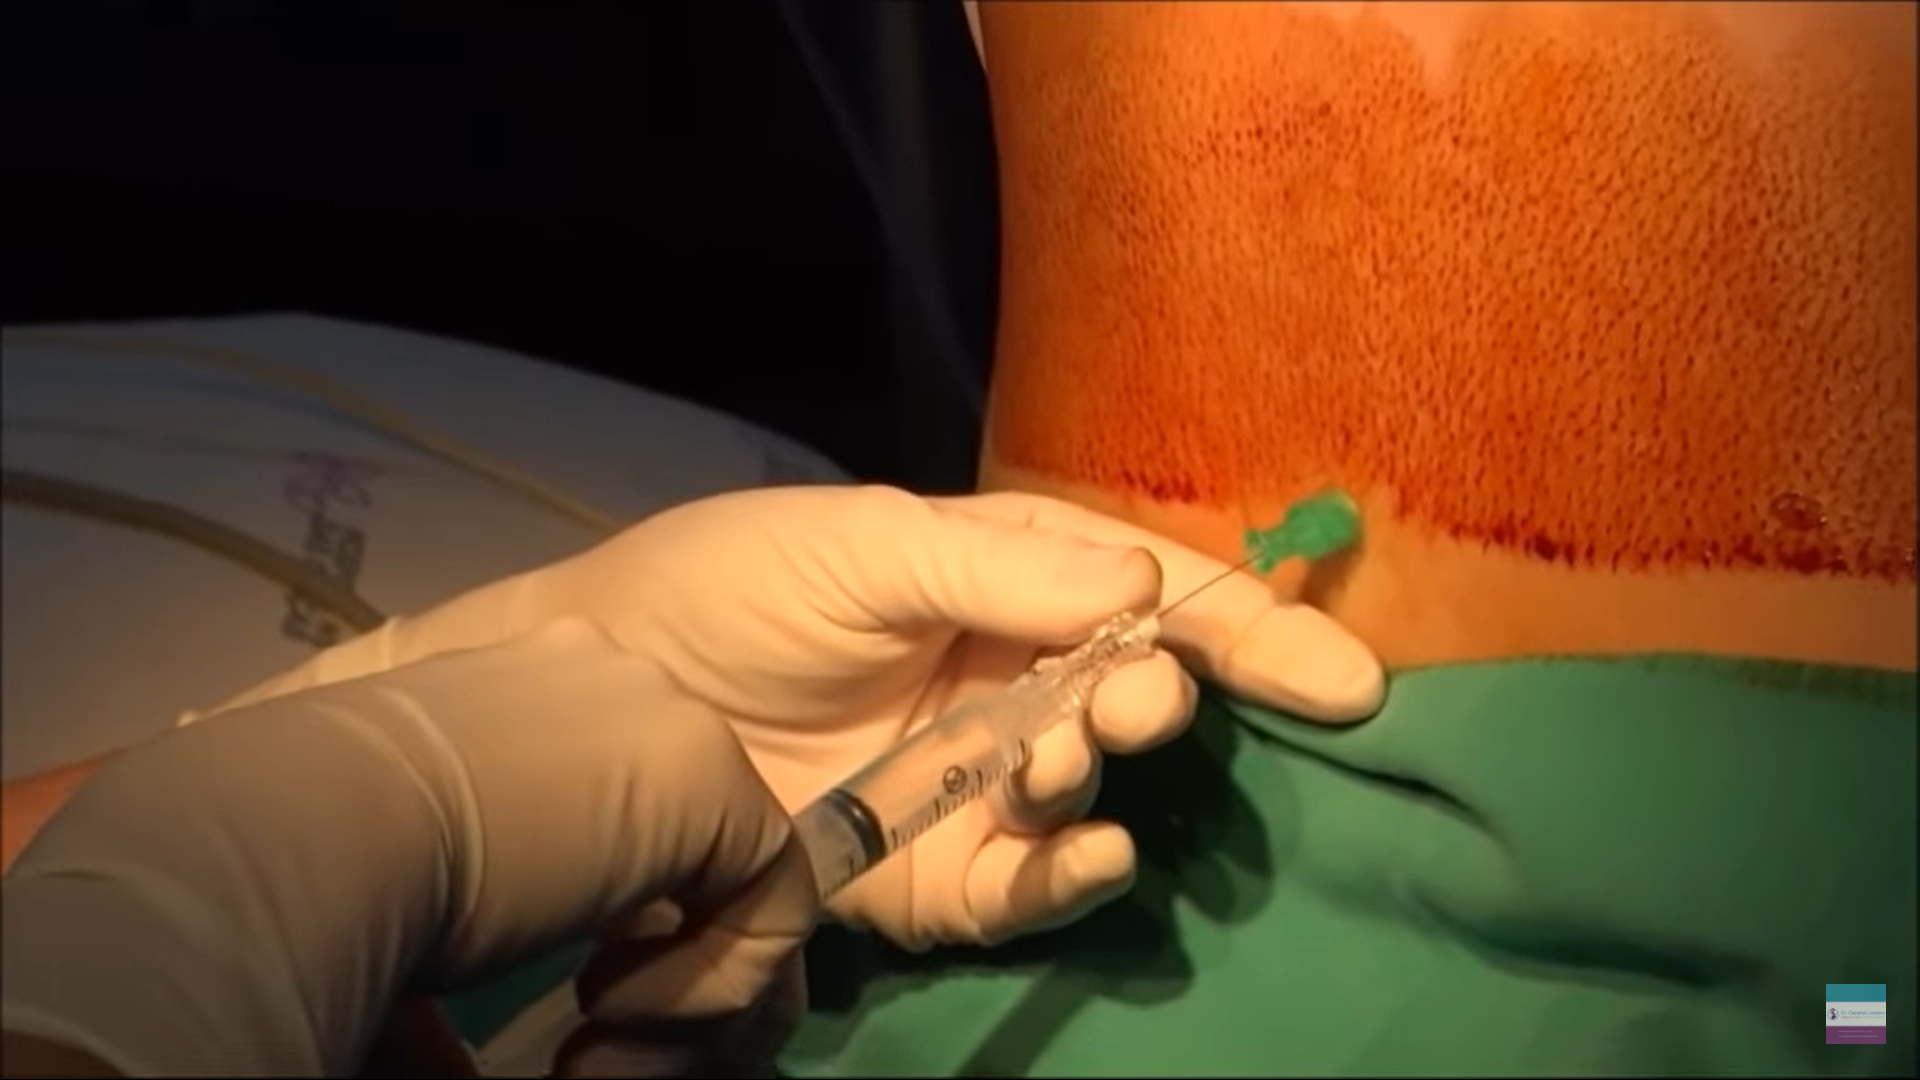
\includegraphics[width=0.6\linewidth]{capitulos/figuras/4.InjecaoAnestesico.png}
    \caption{Injeção do liquido anestésico no espaço subaracnóideo  \cite{Londero2018}.}
    \label{fig:injecaoAnestesico}
\end{figure}

Após a finalização dos procedimentos de preparação é escolhida a área onde será feita a punção através do toque da mão do médico (exemplo retirado de video na Figura~\ref{fig:marcacaoPonto}) na crista ilíaca do paciente \cite{Helayel2010,Isaacs2015}. Uma vez escolhido este ponto é feita a injeção de anestésico local (Figura~\ref{fig:anestesiaLocal}) para reduzir o desconforto na área próxima à punção \cite{Sedicias2018} Após a anestesia local é feita a inserção da agulha de punção tanto no caso da peridural como na raqui.

Existem duas principais abordagens de inserção da agulha para efetuação das anestesias regionais. Estão são denominadas mediana (do inglês \textit{midline}) e paramediana (do inglês \textit{paramedian}). A abordagem mediana é utilizada com mais frequência (96\%) \cite{Wantman2006}. Um dos motivos para o maior uso da abordagem mediana é a ausência de vasos sanguíneos no caminho da agulha nesta abordagem \cite{Bapat2015}. A abordagem paramediana é mais recomendada para pacientes idosos \cite{Ahsan-ul-Haq2005} por motivos de modificação degenerativa da coluna vertebral \cite{Boon2003} e calcificação dos ligamentos interespinhoso e supraespinhoso \cite{Wantman2006}. A abordagem paramediana também pode ser mais viável que a mediana em pacientes obesos pela dificuldade na identificação da crista ilíaca nestes pacientes. Isto por que a camada de gordura faz com que a linha média seja mais difícil de localizar através do toque do médico \cite{N.2013}. Na abordagem mediana a agulha é inserida na linha média da coluna vertebral. Na paramediana existe certa angulação entre a linha da coluna e a inserção da agulha. As duas abordagens podem ser observadas no corte transversal da coluna na Figura~\ref{fig:abordagensInsercaoAgulha}. 

\begin{figure}[ht!]
    \centering
    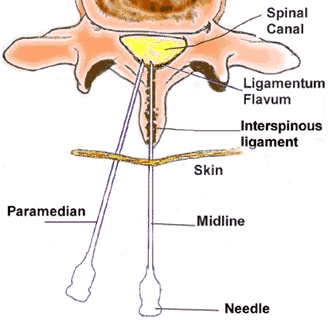
\includegraphics[width=0.6\linewidth]{capitulos/figuras/paramedian-midline-MedBroadcast-Tiff.png}
    \caption{Ilustração da abordagem mediana e paramediana para inserção de agulha \cite{MedBroadcast2018}.}
    \label{fig:abordagensInsercaoAgulha}
\end{figure}

\subsection{Anestesia Raquidiana}

Neste tipo de anestesia, uma agulha de pequeno calibre é inserida nas costas do paciente até atingir o espaço subaracnóideo (localizado após a dura-máter), dentro da coluna espinhal. Em seguida, um anestésico é injetado dentro do líquido cérebro espinhal (\textit{líquor}), produzindo dormência temporária e relaxamento muscular (Figura~\ref{fig:injecaoAnestesico}). Anestesias raquidianas são aplicadas de forma mais frequente em espaços intervertebrais abaixo da segunda vértebra lombar (L2), normalmente entre a L3 e L4 \cite{Wikipedia2019, Londero2018}. A Figura~\ref{fig:camadasPuncaoLombar} ilustra em um corte sagital da coluna as diferentes camadas que são cruzadas por uma agulha durante o procedimento de punção lombar até chegar ao espaço subaracnóideo. Considerando as duas abordagens de inserção da agulha (mediana e paramediana) as camadas onde a agulha pode passar desde a pele até o espaço subaracnóideo são: gordura subcutânea, músculo, ligamento supraespinhoso, ligamento interespinhoso, ligamento amarelo (\textit{flavum}), espaço epidural e dura-máter. O processo espinhoso que também aparece entre a pele e o espaço subaracnóideo na Figura~\ref{fig:camadasPuncaoLombar} não foi listado, pois, por ser uma camada de osso, ela não é perfurada pela agulha e sim uma camada intransponível em relação ao processo de punção.

\begin{figure}[ht!]
    \centering
    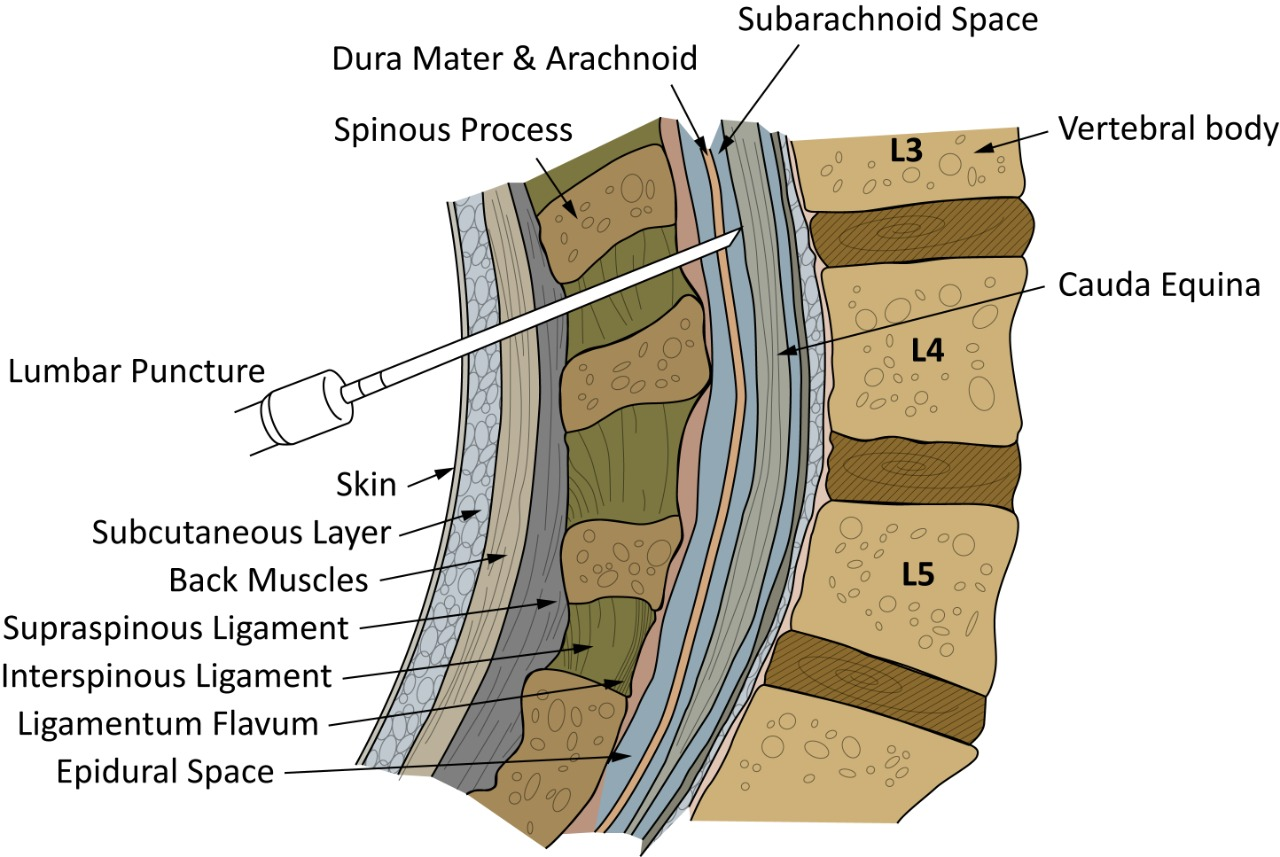
\includegraphics[width=0.6\linewidth]{capitulos/figuras/lumbar.puncture.tisssues.jpeg}
    \caption{Camadas cruzadas pela agulha numa punção lombar.}
    \label{fig:camadasPuncaoLombar}
\end{figure}

A ação do anestésico dentro da coluna espinhal é a de bloquear os nervos que passam pela coluna lombar, fazendo com que os estímulos dolorosos vindos de membros inferiores e do abdômen não cheguem ao cérebro. A raquianestesia é muito usada para procedimentos ortopédicos de membros inferiores assim como na região abdominal e cirurgias obstétricas de parto normal e cesarianas \cite{Pinheiro2018}.

A grande vantagem da anestesia raquidiana em relação a peridural é que nesta é necessário o uso de uma pequena quantidade de anestésico local. Esta característica reduz consideravelmente o risco de intoxicação por meio do elemento anestésico. Por outro lado a maior desvantagem no uso deste tipo de anestesia está na dor de cabeça que os pacientes sentem após a perfuração da dura-máter. Este sintoma é causado pela lesão na dura-máter que pode permanecer aberta por alguns dias após o procedimento, provocando perda do \textit{líquor} do espaço subaracnóideo. Com o uso de agulhas de menor diâmetro a incidência desta dor de cabeça foi consideravelmente reduzida \cite{INFOESCOLA2018}. 

\section{Realidade Virtual}

A \acrlong{RV} está presente quando se usa a tecnologia para criar a ilusão de que se está em um ambiente que não está lá ou não existe. Ela é uma aproximação da realidade experimentada por nós através dos nossos sentidos e sistemas de percepção. A nossa percepção da realidade vem através dos nossos sentidos. Portanto, uma vez apresentando aos sentidos às informações esperadas, sendo estas reais ou não, a nossa percepção da realidade irá se guiar por estes estímulos. Os sentidos mais comuns são visão, olfato, paladar, audição e tato. Porém também possuímos outros sentidos que afetam as nossas percepções do mundo, como por exemplo: o senso de equilíbrio, o sentimento de forças, pesos e deslocamentos sentidos por nossos membros \cite{VRS2018}.

Atualmente, a chamada \acrfull{RV} utiliza um computador para criar um ambiente virtual tridimensional. A intenção é a de simular uma realidade apresentando os elementos desejáveis para os sentidos do usuário, visando cumprir um objetivo através da interação de um ou mais usuários com este ambiente. Estes usuários se tornam parte deste ambiente virtual, total ou parcialmente, podendo manipular objetos ou executar um conjunto de ações \cite{VRS2018}.

A \acrshort{RV} possui uma série de usos sociais como, por exemplo, o tratamento de fobias. Há trabalhos para aracnofobia \cite{Carlin1997}, para aicmofobia ou medo de agulhas \cite{Galoustian2018}, para aerofobia ou medo de voar \cite{Rothbaum2006}, para acrofobia ou medo de altura \cite{Edwards2018} ou de forma mais geral para o medo e a ansiedade \cite{Goldman2017}. A Figura~\ref{fig:medoAltura} ilustra a aplicação para tratamento da acrofobia. Em primeiro plano a usuária com os óculos de realidade virtual e no segundo plano o ambiente virtual simulando ambientes de escadas e plataformas com fundo transparente.

\begin{figure}[ht!]
    \centering
    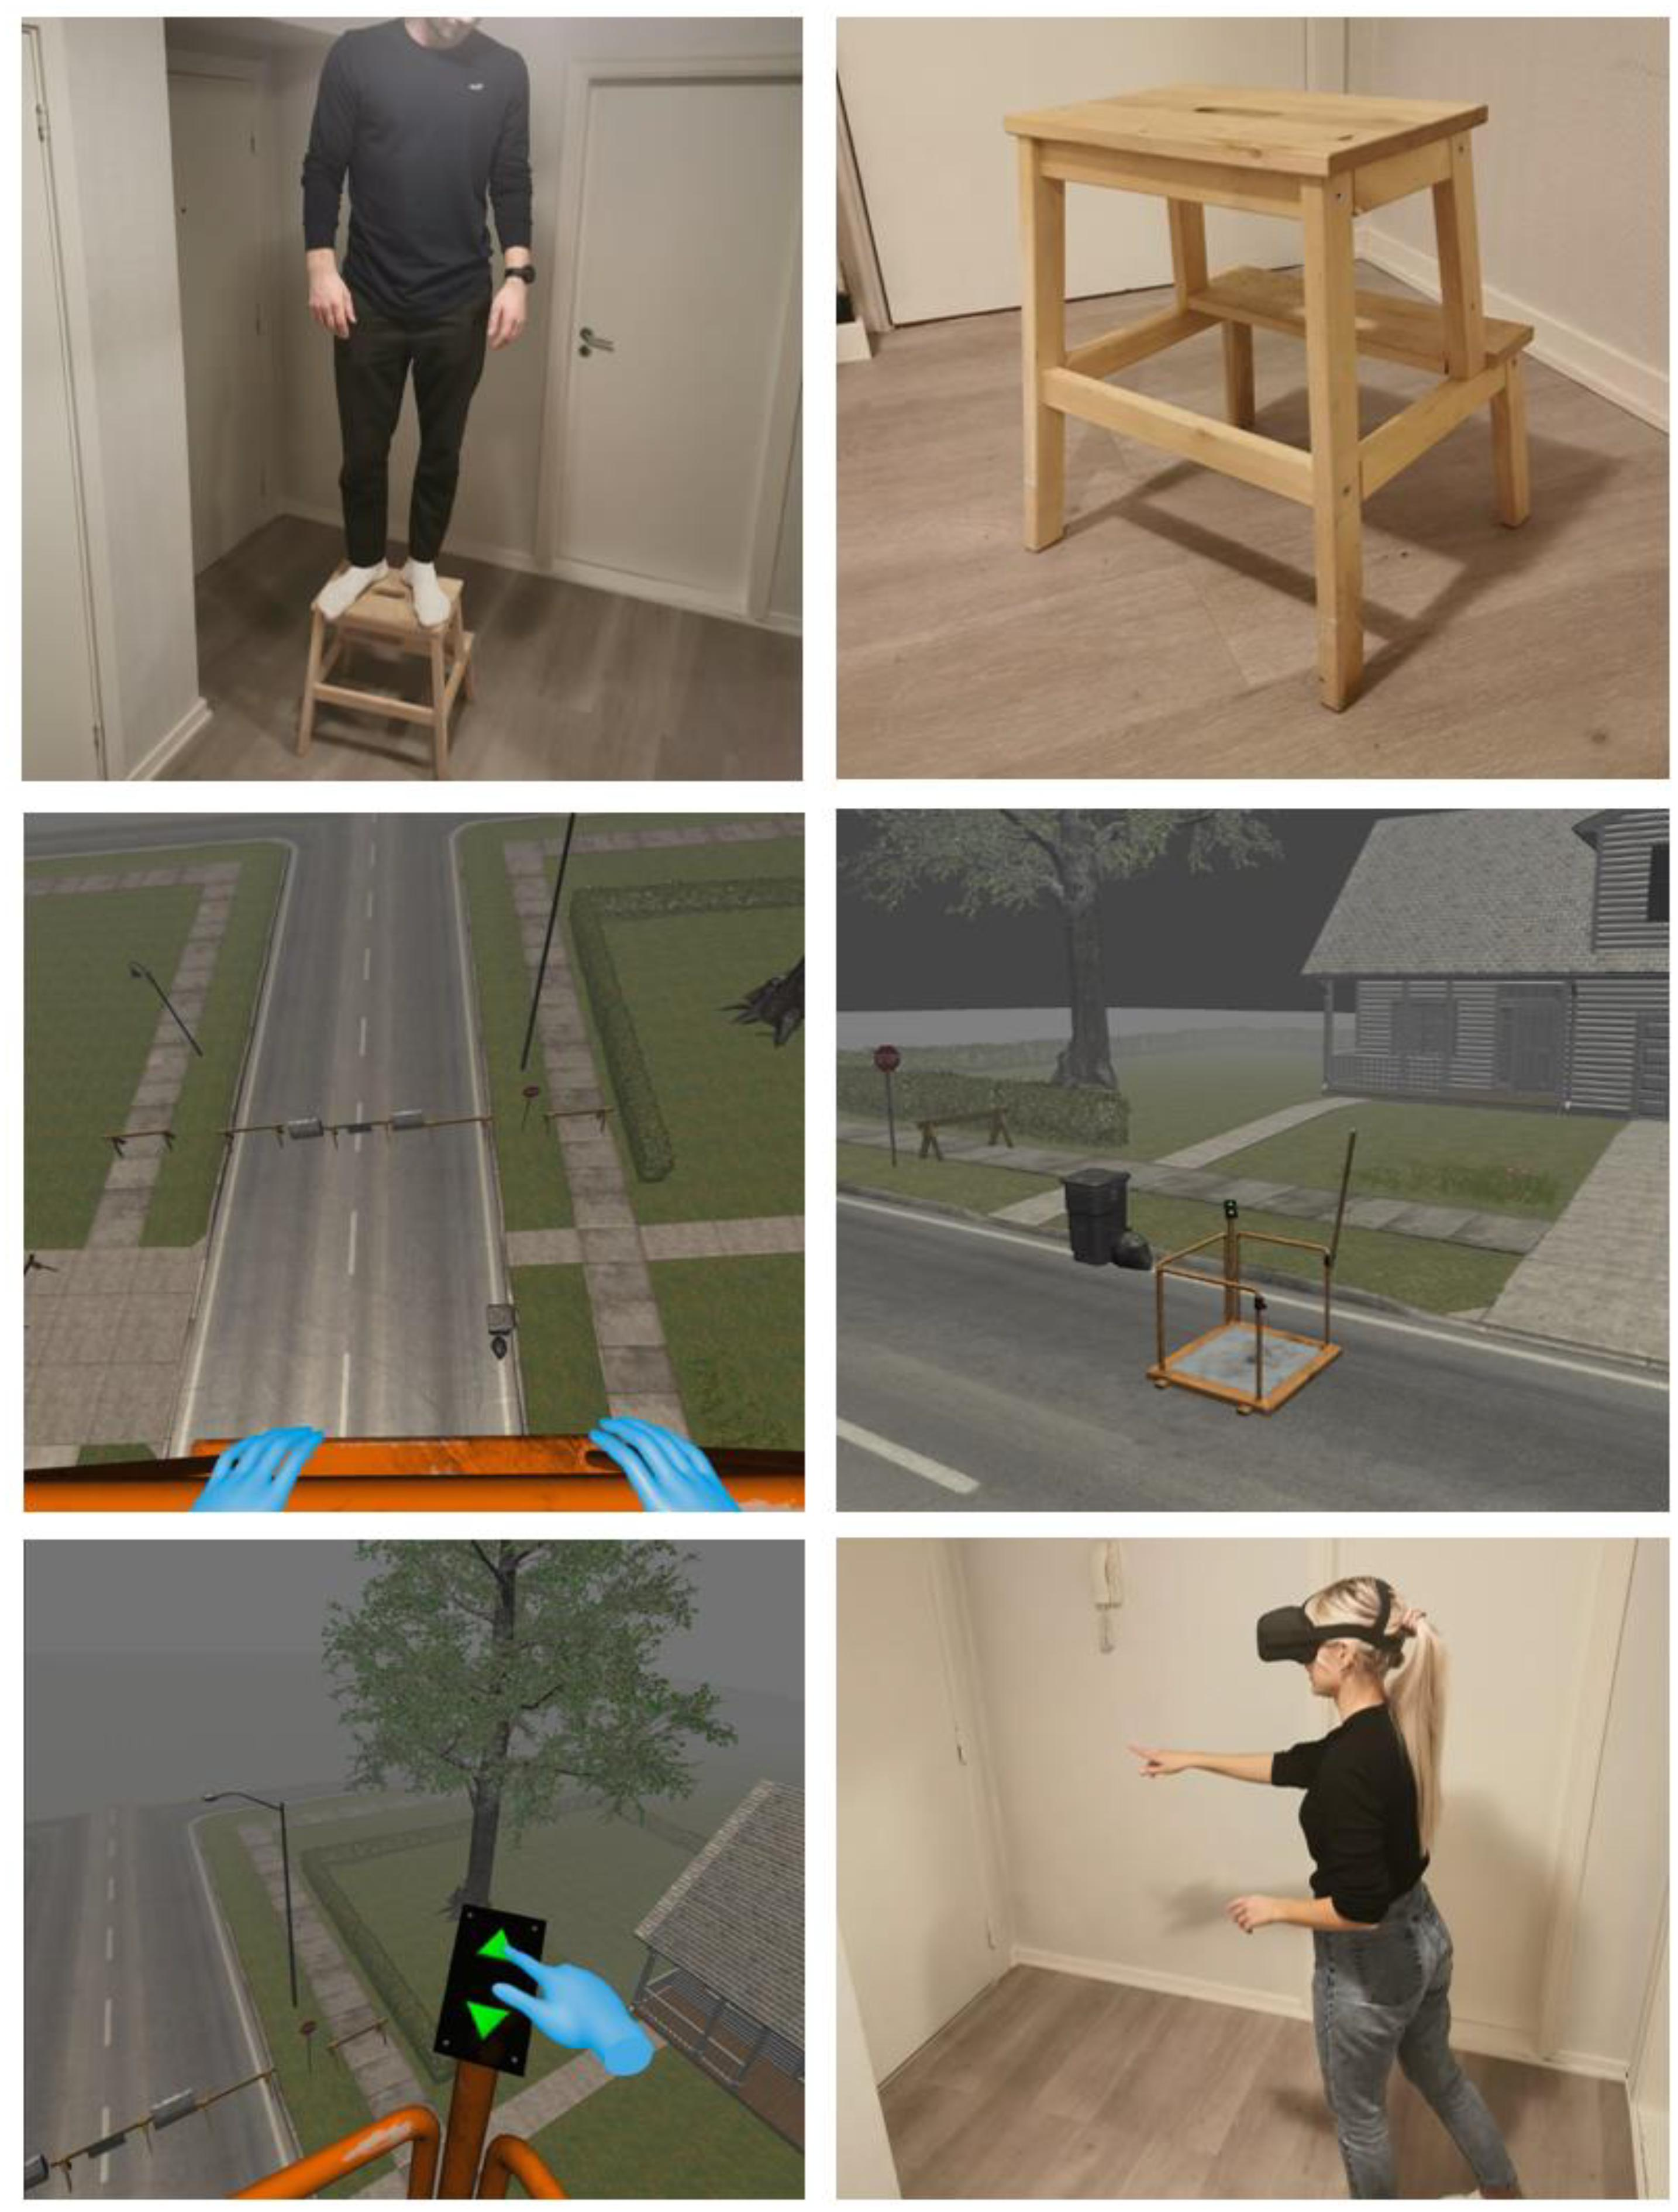
\includegraphics[width=0.6\linewidth]{capitulos/figuras/fear_of_heights.jpg}
    \caption{Exemplo de aplicação que usa \acrshort{RV} no tratamento da acrofobia \cite{Edwards2018}.}
    \label{fig:medoAltura}
\end{figure}

A indústria do entretenimento através de filmes e jogos provocou uma grande evolução de técnicas de \acrshort{RV} que posteriormente foram aplicadas em áreas mais “sérias” como o desenvolvimento pessoal e treinamento \cite{Ma2011, Prensky2001, Smith2011}. Na prática a \acrshort{RV} deve ser considerada como uma possibilidade sempre que o que se deseja fazer é muito perigoso, caro ou impraticável de ser realizado concretamente. Por conta destas características ela é muito usada nas áreas da educação, da saúde e militar \cite{VRS2018}. Conforme a tecnologia que permite a criação e simulação de ambientes virtuais se torna mais barata, mais aplicações são criadas com o uso destas ferramentas.

\section{Dispositivos Hápticos}

O termo \textit{haptics} é usado para descrever a ciência que estuda e simula a pressão, textura, vibração e outras sensações biológicas relacionadas ao toque. A sensação do toque se origina em estímulos mecânicos, elétricos, térmicos ou químicos na pele \cite{Burdea1996}. O tato não está localizado numa região específica do corpo como os demais sentidos. Ele está distribuído por todo o corpo através do órgão sensorial do toque, nossa pele, articulações, músculos e tendões. O senso do toque se divide em duas sensações: cinética e tátil. Forças e torques são sensações cinéticas que sentimos nos músculos, tendões e articulações. Já as sensações táteis como pressão, deformação e vibração são sentidas por mecano receptores que possuímos na nossa pele \cite{Culbertson2018}. 

Os primeiros dispositivos hápticos foram originados dos braços robóticos usados para o controle remoto de robôs \cite{Zurawski2005} As aplicações de tecnologias hápticas são muito variadas envolvendo, por exemplo, projetos de engenharia e aplicações de manufatura \cite{Sharma2001}, entretenimento (videogames e filmes), celulares, relógios inteligentes e até mesmo a indústria automobilística \cite{Smith2019}. Estes dispositivos possuem elementos mecânicos de entrada e saída para interação com o usuário. Uma ou mais partes do dispositivo em contato com o usuário são monitorados no espaço físico e o dispositivo oferece como retorno força e torque. Desta forma um canal bidirecional de interação entre o ambiente virtual e o usuário é criado \cite{Coles2011}. Estes dispositivos estão sendo cada vez mais utilizados hoje em dia tanto pela evolução da sua tecnologia como pela diminuição dos preços. Com o avanço da tecnologia estes dispositivos estão se tornando cada vez mais flexíveis representando mais fielmente os movimentos. Isto ocorre  através do uso de conceitos de restrição parcial a movimentos, deslocamentos e da inclusão de mais graus de liberdade, \textit{\acrfull{DoF}}. 

O número de graus de liberdade de um dispositivo háptico se refere ao número de maneiras diferentes em que este pode se mover ou criar forças. Como exemplo, dispositivos com 3 graus de liberdade podem rastrear posições e criar forças ao serem movidos nas direções: direita-esquerda, frente-trás e cima-baixo \cite{HAPTICSHOUSE2019}. O principal objetivo no uso destes dispositivos é o aumento da sensação de imersão em um ambiente de realidade virtual. 

Em relação à área médica, os dispositivos hápticos vem sendo utilizados na maioria dos trabalhos de simulação de procedimentos médicos \cite{Coles2011,Escobar-Castillejos2016}. Eles são usados para simular o uso de ferramentas em cirurgias e ajudaram a impulsionar o sucesso das práticas em simuladores virtuais. Isto aconteceu ao proporcionar o controle dos graus de liberdade de deslocamentos, a restrição aos movimentos e as respostas às atitudes do usuário como forças de reação ou \textit{feedback} \cite{Gerovich2004}. Estes dispositivos eletromecânicos existem nas mais diversas formas e são adaptados para uma grande variedade de procedimentos médicos como, por exemplo, no treinamento de laparoscopia \cite{Srinivasan2004}, biopsia de próstata \cite{Sclaverano2009}, cirurgia de fígado \cite{Mastmeyer2016}, exames de mama \cite{Brazil2017,Jeon2010,Ribeiro2014,Solanki2010}, simulação de apalpação \cite{Ribeiro2016} e punções epidurais \cite{N.2013, Brazil2018}. Alguns sistemas usam mais de um háptico como em punções de agulha guiadas por ultrassom que usam um equipamento para simular a agulha e outro para o ultrassom \cite{Ni2011,Vidal2008}. Outros chegam a fazer o uso de três dispositivos como o PalpSim de forma a simular o toque das mãos do usuário num paciente virtual \cite{Coles2011b}. 

Culbertson et al. identificaram como 3 as principais categorias de sistemas hápticos: compreensíveis, vestíveis e palpáveis. Um exemplo visual destes tipos pode ser visto na Figura 6. Os sistemas compreensíveis são dispositivos tipicamente cinéticos (\textit{feedback} de força) que normalmente possuem uma base fixa e permitem ao usuário empurrar e ser empurrado de volta. Sistemas vestíveis são tipicamente táteis montados nas mãos ou em outras partes do corpo e provocam sensações diretamente na pele. Os sistemas palpáveis são dispositivos de encontro que permitem ao usuário explorar toda a superfície \cite{Culbertson2018}. Os dispositivos a serem explorados aqui são os de sistemas compreensíveis. Estes foram os tipos de hápticos utilizados nos simuladores computacionais relacionados ao tema desta tese (seção 0) assim com nos diversos outros simuladores médicos estudados e citados nesta seção. Ribeiro et al. fizeram uma revisão sobre dispositivos usados na simulação de procedimentos que envolvem o toque da mão do médico para identificação de características e anormalidades sob a pele \cite{Ribeiro2016}. Os autores analisaram 57 trabalhos e mais da metade fez uso dos dispositivos da família \textit{Phantom}. Os dispositivos desta família serão listados na seção ===== 3 ======.

===== FIGURA ====

Nas figuras Figura 7, Figura 8, Figura 9 e Figura 10 os dispositivos aparecem representados ordenados pelas suas complexidades i.e. dos mais simples (mais antigos e com menos recursos) aos mais avançados (mais novos). Todos estes dispositivos são exemplos de sistemas tipicamente cinéticos. Os mais novos possibilitam maior número de graus de liberdade para os movimentos assim como possibilitam mais forças e momentos de reação. O Novint Falcon ® (Figura 7), lançado em 2007, tem como interface com o usuário uma esfera onde o usuário deve colocar os dedos da mão para fazer os movimentos no caso do seu uso mais comum. No que diz respeito à liberdade de movimento este mecanismo proporciona uma interação 3D com o computador no lugar da interação 2D proporcionada pelo mouse. Ele possui 3 graus de liberdade de movimento e de forças. Nesta esfera existem quatro botões para interação e existem sensores para determinar a posição do cursor e motores para controlar as forças a serem transmitidas para o usuário. Existem versões onde a esfera é substituída, por exemplo, por um dispositivo semelhante a uma pistola para que o dispositivo seja usado em jogos de tiros de primeira pessoa \cite{VRS2017}. 

===== FIGURA ====

Os hápticos da família \textit{Phantom Geomagic Touch} ® (Figura 8) e \textit{Geomagic Touch} X ® (Figura 9) apresentam uma peça que simula uma caneta para manipulação do usuário da mesma forma que a esfera no dispositivo da Figura 7. Nas canetas também existem botões para interação e da mesma forma estas também são substituíveis por partes com formas mais adequadas ao procedimento que estas pretendem simular. O dispositivo \textit{Geomagic Touch} X ® possui a mesma liberdade de movimento do \textit{Geomagic Touch} ®, porém possibilita \textit{feedback} de reações maiores. Ambos apresentam 6 graus de liberdade de movimento e 3 graus de liberdade no retorno de forças. Estes dispositivos, portanto mapeiam a posição 3D e orientação, mas somente apresentam \textit{feedback} de forças direcionais \cite{Forsslund2013}.

===== FIGURA ====

===== FIGURA ====

O \textit{Phantom Premium} ® (Figura 10) está disponível nas versões \textit{Premium} 1.0, \textit{Premium 1.5} e 1.5/HF, e \textit{Premium} 3.0. Estas evoluem não só o \textit{feedback} de reações como também os graus de liberdade dos movimentos. Enquanto o \textit{Phantom Premium} 1.0 ® simula o movimento do giro do pulso na mão o \textit{Phantom Premium} 3.0 ® possibilita uma amplitude que simula os graus de liberdade de movimento de todo o braço humano desde o ombro \cite{3DSystems2018}. Este dispositivo possui 6 graus de liberdade tanto para movimento como retorno de forças o que o torna simétrico no número de sensores e motores (atuadores). São computadas forças e torques tanto da posição como da orientação deste dispositivo. Esta característica tem uma forte influencia no alto custo associado a este tipo de dispositivo \cite{Forsslund2013}.

===== FIGURA ====

=========

\section{Modelagem de tecidos}

Um dos passos necessários para construção de um ambiente virtual para treinamento de anestesia epidural e raquianestesia é a criação de pacientes virtuais. Um importante aspecto da modelagem destes pacientes é como eles aparecem na tela da aplicação. Outro aspecto importante na simulação é ter uma estimativa da espessura dos tecidos envolvidos nestes tipos de anestesia. Para isto é necessária à modelagem do tamanho de todas as camadas de tecido pelos quais as agulhas passam para execução destes procedimentos. Uma ilustração destes tecidos que vão desde a pele até a dura-máter pode ser vista na Figura 3. Nesta seção são descritos trabalhos relacionados com a modelagem da distância entre a pele e a dura-máter.

Na Tabela 2 são listadas as varáveis de entrada e saída dos métodos estudados nesta seção. Esta tabela exibe também as unidades destas variáveis que serão utilizadas em todo este trabalho.

===== TABELA ====

Muitos trabalhos buscam relacionar a distância que vai da superfície externa da pele até o espaço epidural (DEE) com as demais variáveis da Tabela 2. A grande maioria dos trabalhos indica uma forte relação da DEE com o IMC \cite{Adegboye2017, Galbraith2018}. Estes dois trabalhos não fazem separação dos grupos populacionais por idade, sexo ou etnia, e usaram populações respectivamente de n=120 e n=317 pessoas entre homens e mulheres.

Os trabalhos citados a seguir analisaram somente ou de forma separada grupos de mulheres grávidas. Como este é o foco deste trabalho só serão comentadas aqui as conclusões referentes a estes grupos. Todos os trabalhos a seguir encontraram influencia do IMC na determinação da DEE, mas além desta relação também foram encontradas outras combinações em cada trabalho. O grupo étnico/populacional do individuo foi observado em conjunto com o IMC em \cite{Sharma2011} estudo feito no Reino Unido. A idade foi observada em conjunto com o IMC num estudo em pacientes americanas em Michigan, EUA \cite{Clinkscales2007}. A altura, massa, idade e IMC foram observados como relevantes em um estudo em pacientes da Índia \cite{Hazarika2016}. Estes dois últimos trabalhos construíram equações de regressão linear para determinação da DEE para grupos de parturientes conforme pode ser visto na Tabela 3.

===== TABELA ====

Os autores em \cite{Sharma2011} no lugar das equações apresentaram como resultado uma tabela com cinco pontos de cada par IMC x DEE para cada grupo populacional analisado. Estes dados podem ser vistos na Tabela 4. A definição dos grupos populacionais no estudo do Reino Unido (RU) em \cite{Sharma2011} foi: Brancas (população do Reino Unido, da Irlanda e qualquer outro grupo com cor de pele branca); Asiáticas ou Britânicas Asiáticas (população da Índia, Paquistão, Bangladesh ou qualquer outro grupo Asiático); Negras ou Britânicas negras (população de Africanas, Caribenhas ou outros grupos com cor da pele negra); e Chinesas e outros grupos étnicos (população da China, Japão, Malásia, Filipinas etc.). No grupo de nome Chinesas, além dos dados de pessoas desta origem moradoras do Reino Unido, foram considerados dados de Chinesas (n=70) de um hospital de Singapura.

===== TABELA ====

Na Tabela 5 é apresentado o tamanho da população utilizada nestes estudos e as identificações da origem dos dados do estudo, isto é, os grupos populacionais analisados. 

===== TABELA ====

A listagem dos tecidos entre a pele e a DEE e a relação dessa distância com o aumento de peso é comentada em \cite{Palmer1983}. Os autores concluem que com o aumento do peso/massa (do paciente) o tecido que sofre a maior variação é a gordura subcutânea.

Na seção = ==== é proposto o uso de dados de trabalhos comentados aqui para modelagem de tecidos de pacientes grávidas.

=========

Este capítulo apresentou uma fundamentação teórica sobre ====. Iniciou apresentando ==========. Logo em seguida o capítulo apresenta ====== e suas principais entidades e que estão relacionadas com a proposta desta tese. O capitulo finaliza apresentando os conceitos que envolvem ==== e seus principais elementos. O próximo capítulo oferece uma visão das pesquisas relacionadas ao tema desta tese e compara-as com as proposições que foram colocadas ao longo deste trabalho. Essas pesquisas tratam e ========== assim como de ===========.


% --- -----------------------------------------------------------------
% --- Referencias Bibliograficas. (Obrigatorio)
% --- -----------------------------------------------------------------
\cleardoublepage

 %para personalização da bibliografia olhar os PDFs na pasta "MANUAIS"
\printbibliography[
   % heading=bibintoc,
    title={REFERÊNCIAS} %TITULO DA SEÇÃO
] 

% --- -----------------------------------------------------------------
% --- Apendice.(Opcional)
% --- -----------------------------------------------------------------
\cleardoublepage
\appendix
%para melhor organização deixar os Anexos e Apêndices na pasta anexos.
\chapter{Projeto aprovado no comitê de ética via plataforma Brasil}
\label{apend}

\begin{figure}[htp] \centering{
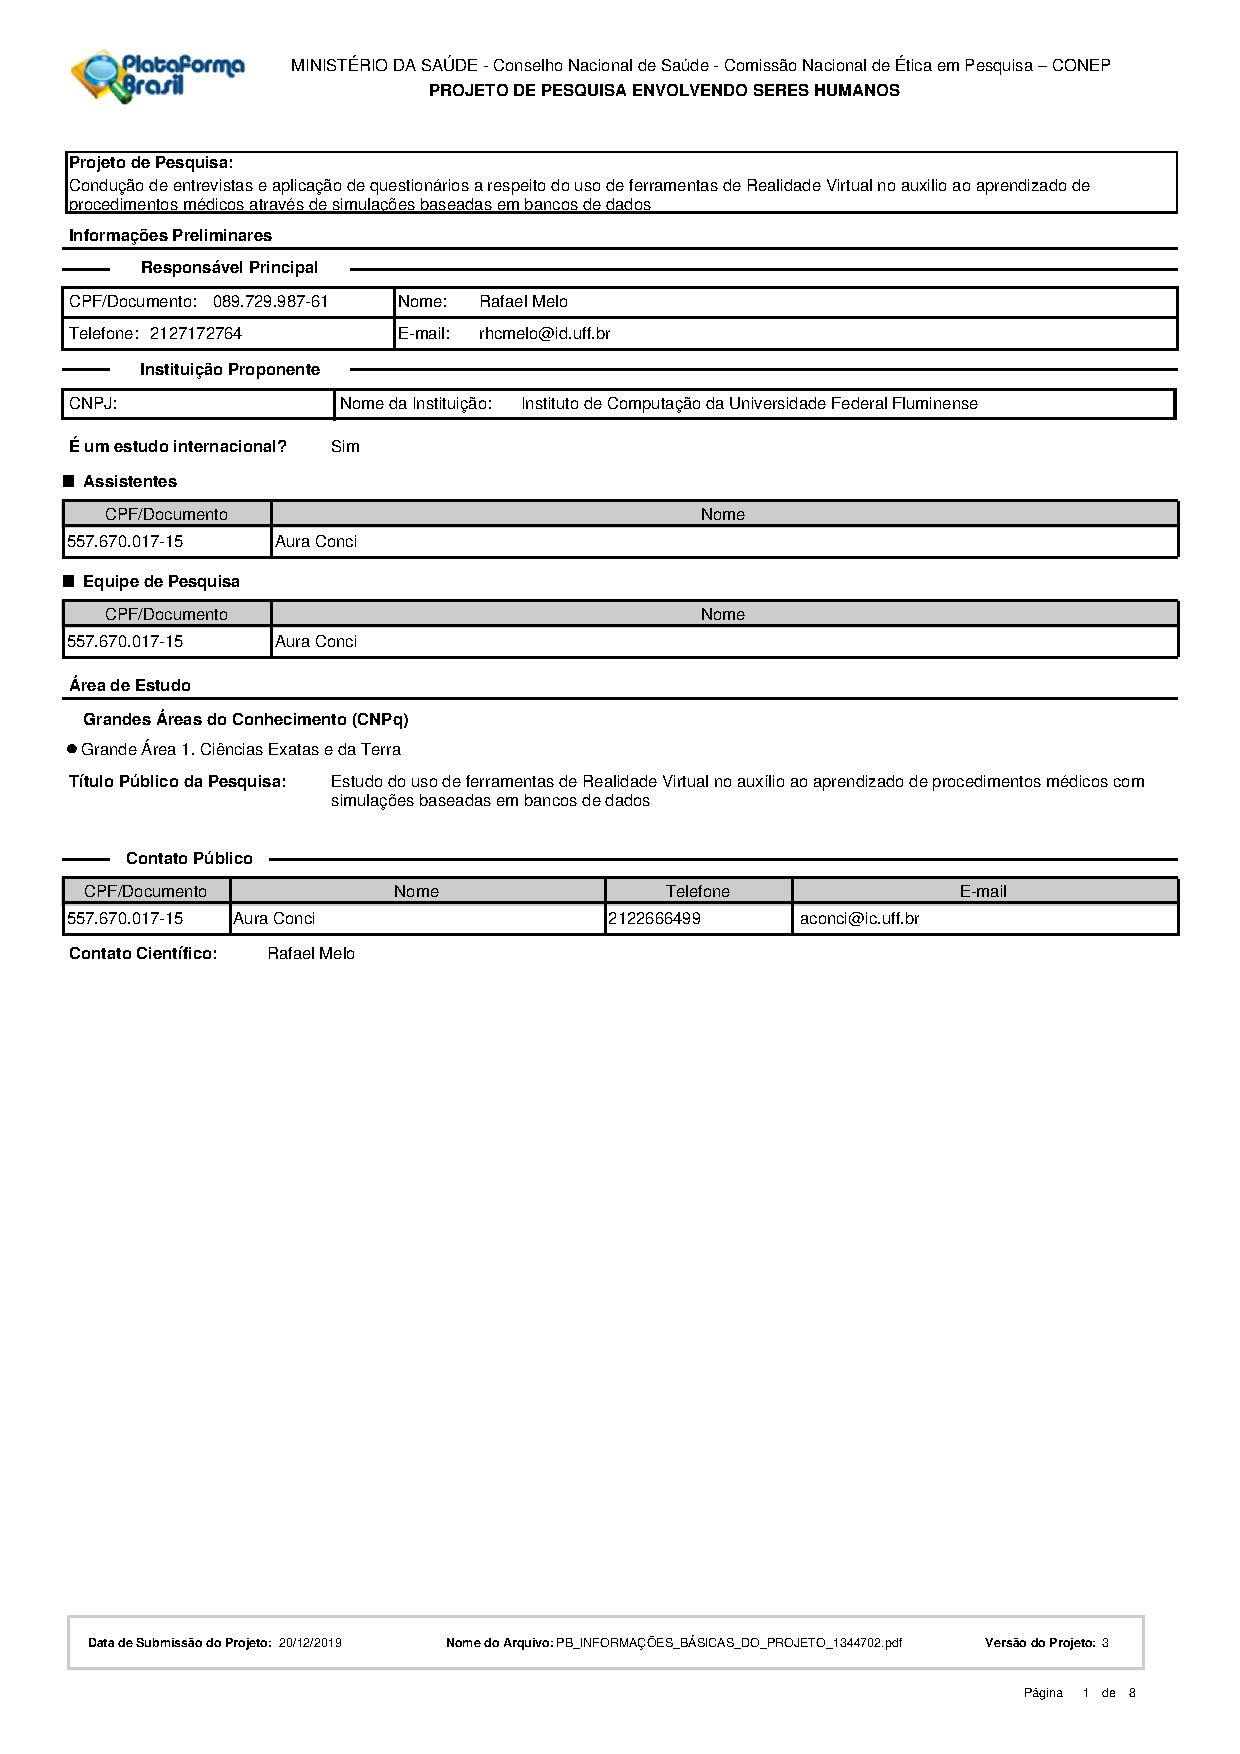
\includegraphics[scale=0.82]{pos-textuais/apendices/PB_INFORMAÇÕES_BÁSICAS_DO_PROJETO_1344702.pdf}
\caption{Experiment 1}
\end{figure}

% Este apêndice apresenta informações complementares.

%Elemento opcional. O(s) apêndice(s) são identificados por letras maiúsculas consecutivas, travessão e pelos respectivos títulos. Excepcionalmente utilizam-se letras maiúsculas dobradas, na identificação, quando esgotadas as 23 letras do alfabeto (ABNT, 2005).



%\chapter{ANEXO A – TÍTULO DO ANEXO}
\label{lab:anexoA}

"Elemento opcional. O(s) anexo(s) são identificados por letras maiúsculas consecutivas, travessão e pelos respectivos títulos. Excepcionalmente utilizam-se letras maiúsculas dobradas, na identificação dos anexos, quando esgotadas as 23 letras do alfabeto" (ABNT, 2005).


\end{document}

